\chapter{铁碳合金的显微组织观察及性能分析}
\section{实验目的}
\begin{enumerate}
    \item 了解金相显微镜的成像基本原理、构造、主要部件及作用;
    \item 熟悉金相显微镜的使用和其注意事项;
    \item 掌握分析铁碳合金在平衡状态下及不同工艺热处理后的显微组织形态;
    \item 加深理解铁碳合金组织与性能之间的关系。
\end{enumerate}

\section{实验原理}%简单描述,含必要的公式和附图;
    \subsection{金相显微镜的成像原理}
        显微镜不似放大镜那样由单个透镜组成,而是由两级特定透镜所组成。靠近被观察物体的透镜叫做物镜,而靠近眼睛的透镜叫做目镜。借助物镜与目镜的两次放大,就能将物体放大到较高的倍数($\sim 2000$倍)。\fgref{fig:microscope} 所示是在显微镜中得到放大物像的光学原理图。被观察的物体 $AB$ 放在物镜之前距其焦距略远一些的位置,由物体反射的光线穿过物镜,经折射后得到一个放大的倒立实像 $A^{'}B^{'}$,目镜再将实像 $A^{'}B^{'}$ 放大成倒立虚像 $A^{''}B^{''}$,这就是我们在显微镜下研究实物时所观察到的经过二次放大后的物像。在设计显微镜时,让物镜放大后形成的实像 $A^{'}B^{'}$ 位于目镜的焦距 $f$ 目之内,并使最终的倒立虚像 $A^{''}B^{''}$ 在距眼睛 \SI{250}{\mm} 处成像,这时观察者看得最清晰。此时 $A^{''}B^{''}$ 的放大倍数是物镜放大倍数与目镜放大倍数的乘积。
        \begin{figure}[!ht]
            \caption{显微镜光学原理图\label{fig:microscope}}
            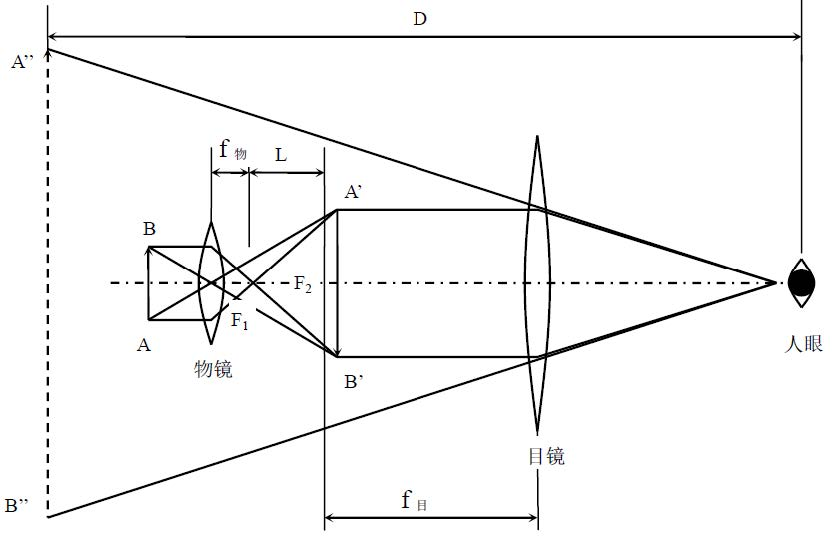
\includegraphics[width=0.7\textwidth]{img/A1/microscope.jpg}
        \end{figure}\par
        显微镜的放大倍数为
        \begin{equation}
            M=M_\text{物}\cdot M_\text{目}\approx\frac{\Delta}{f_1}\cdot\frac D{f_2}
            \label{equ:A1.1}
        \end{equation}\par
        式中:
        \begin{minipage}[t]{100mm}
            $M_\text{物}$-物镜的放大倍数;\par
            $M_\text{目}$-目镜的放大倍数;\par
            $f_1$-物镜的焦距;\par
            $f_2$-目镜的焦距;\par
            $\Delta$-显微镜的光学镜筒长(即物镜后焦点到所成实像的距离);\par
            $D$-人眼明视距离,约为 \SI{250}{\mm}。\par
        \end{minipage}
    \subsection{金相显微镜的构造}
        金相显微镜由照明系统、光学系统和机械系统三部分组成。另有一些显微镜还配有照相装置等附件。
        \subsubsection{照明系统}
            在显微镜底座内装有一个低压灯泡作为光源,与聚光镜、孔径光阑、视场光阑及反光镜组成显微镜的照明系统,使样品表面获得充分均匀的照明。
        \subsubsection{显微镜调焦装置}
            显微镜体两侧有粗调及微动调焦旋钮。转动粗调焦旋钮可使载物台迅速升降,微动调焦旋钮可使物镜缓慢地上下运动,以便精确调焦。
        \subsubsection{孔径光阑(AS)}
            光路中装有两个光阑。孔径光阑的作用是控制入射光束的大小,缩小孔径光阑可以减小像差,增大景深和衬度,使映像清晰。但随着孔径角的缩小,物镜的数值孔径降低,进而会使物镜的分辨能力降低;增大孔径光阑,入射光束变粗,物镜的孔径角增大,可使光线充满物镜的后透镜,数值孔径可达到物镜体上标刻的 NA 值,分辨率会随之提高。但由于球面像差的增加以及镜筒内部反射及炫光的增加,成像质量将降低。因此孔径光阑使用时需做适当的调节,实际操作中以在目镜筒内看到孔径光阑在物镜后焦面上成像达物镜孔径的 $80-90\%$ 时为好。更换物镜后,孔径光阑需做适当调节。另外,不应用它来调节视场的亮度。
        \subsubsection{视场光阑(FS)}
            通过调整视场光阑,可改变显微镜视场大小,可提高映像衬度而不影响物镜的分辨能力。适当调节视场光阑的大小还可减少镜筒内的反射及炫光,提高成像质量。但需注意视场光阑缩得太小,会使观察范围太窄,一般应调节到与目镜视场大小相同。
        \subsubsection{滤色片}
            滤色片是显微镜的辅助部件,通过合理选用可适当提高成像质量。滤色片是由不同颜色的光学玻璃片制成的透明薄片,目的是只允许一定波长的光线通过。其主要有以下几个作用:配合消色差物镜使用黄绿色滤色片,可使像差得到最大限度的校正;对复消色差物镜,可采用蓝色滤色片,由于蓝光波长较黄绿光短,因而可提高物镜的分辨率;减弱光源的强度等。
        \subsubsection{载物台}
            用于放置金相样品,观察面向下。通过调整纵向和横向移动手柄可使载物台在水平面上做一定范围的十字定向运动,以改变试样的观察部位。
        \subsubsection{物镜转换器}
            转换器可安装不同放大倍数的物镜,旋动转换器可使各物镜镜头进入光路,与不同的目镜搭配使用,以获得各种放大倍数。
        \par
        MDS400 倒置式金相显微镜的外形构造请见\fgref{fig:MDS400}。
        \begin{figure}[!ht]
            \caption{MDS400 倒置式金相显微镜的外形构造\label{fig:MDS400}}
            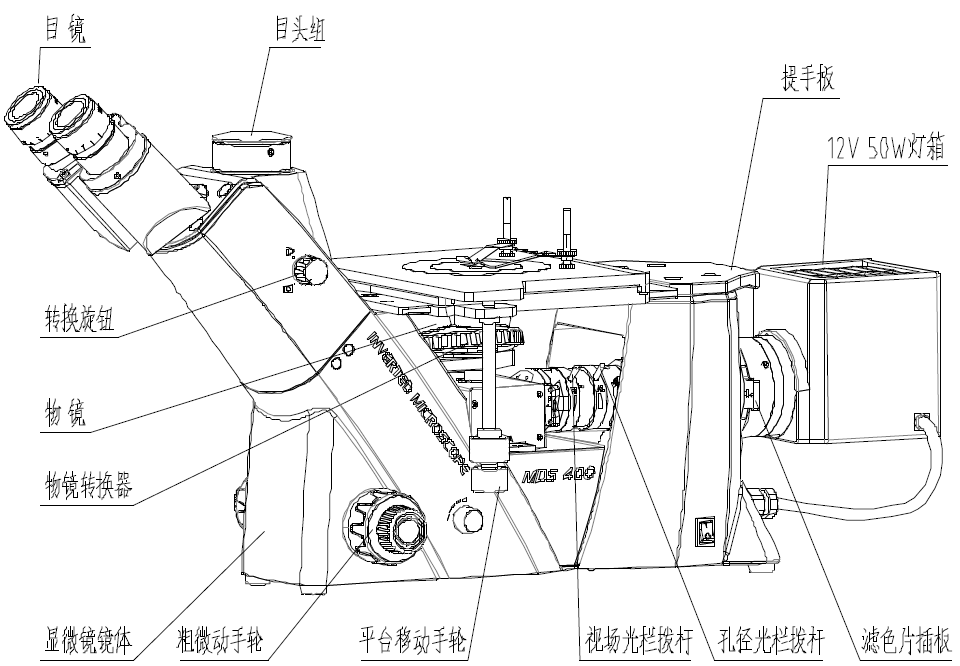
\includegraphics[width=0.83\textwidth]{img/A1/MDS400.png}
        \end{figure}
\section{实验仪器}%规格及参数
    MDS400 倒置式金相显微镜,铁碳合金平衡状态金相试样一套、多种热处理方式之后的碳钢试样一套。
\section{实验过程}%简述主要过程和实验内容
    \subsection{实验内容}
        \begin{enumerate}
            \item 由指导教师结合图例讲解 Fe-C 合金平衡态的基本组织组成、组织的形态特征及金相显微镜的主要结构部件及其作用、基本操作过程及注意事项。
            \item 学生领取一套铁碳合金平衡组织标准试样,按照金相显微镜的操作步骤,在显微镜下观察表中七种铁碳合金平衡组织试样,识别碳钢和铸铁组织形态的特征,建立成分、组织之间相互关系的概念。认真体会整个操作过程,并将观察图像拍照存储。
            \item 学生领取一套经不同热处理工艺的 45 钢及 T12 钢标准试样(21\#-27\#),在显微镜下观察经不同热处理工艺的 45 钢及 T12 试样。理解并分析不同热处理工艺条件下试样的组织变化,认真体会整个操作过程,并将观察图像拍照存储。\par
            其中:\begin{enumerate}
                \item 21\# 为 45 钢 \SI{860}{\degreeCelsius} 水淬 $+$ 中温回火;
                \item 22\# 为 45 钢 \SI{860}{\degreeCelsius} 水淬 $+$ 高温回火;
                \item 23\# 为 45 钢 \SI{780}{\degreeCelsius} 水淬;
                \item 24\# 为 45 钢 \SI{1100}{\degreeCelsius} 水淬;
                \item 25\# 为 T12 钢球化退火;
                \item 26\# 为 T12 钢 \SI{780}{\degreeCelsius} 水淬 $+$ 低温回火;
                \item 27\# 为 T12 钢 \SI{1100}{\degreeCelsius} 水淬 $+$ 低温回火。
            \end{enumerate}
        \end{enumerate}
    \subsection{实验要求}
        \begin{enumerate}
            \item 通过观察金相样品的实际操作过程,学会正确的操作方法,包括物镜和目镜的选择与匹配、调焦、孔径光阑和视场光阑的调节、放大倍数的计算;
            \item 总结金相显微镜的操作要点及必须注意的事项;
            \item 给出所观察试样的显微组织图(显微镜拍摄图及手绘图),手绘图要求画出所观察显微组织示意图,显微组织画在直径为 $25$-\SI{30}{\mm} 的圆内,并标出材料、组织名称及放大倍数。
            \item  分析含碳量对铁碳合金的组织和性能的影响。
        \end{enumerate}
    \subsection{实验注意事项}
        \begin{enumerate}
            \item 操作时必须特别谨慎,不能有任何剧烈的动作,不允许自行拆卸光学系统。
            \item 在旋转粗调或微调旋钮时动作要慢,碰到某种障碍时应立即停止操作,报告指导教师查找原因,不得用力强行转动,否则会损坏机件。
            \item 要爱护已制备好的金相试样。不能用手触摸试样的观察面,如有尘埃等脏物不能用嘴吹,也不能随意擦,要用吸耳球吹除或用无水酒精冲洗并干燥。
            \item 试样观察完毕后要放入干燥箱中保存。
        \end{enumerate}
\section{实验结果}
    \subsection{铁碳合金室温下的平衡组织}
    铁碳合金是研究钢铁材料的基础。工程上广泛应用的碳钢、铸铁都属于铁碳合金。铁碳合金是以铁为主,加入少量的碳而形成的合金。平衡组织是指合金在极为缓慢的冷却条件下(如退火状态)所得到的组织。\par
    \subsubsection{工业纯铁}
    工业纯铁含碳量小于 0.0218\%,室温下的显微组织由白色块状铁素体和极少量的三次渗碳体构成。由于三次渗碳体最多只能达到 0.3\%,通常可忽略不计。用硝酸酒精浸蚀后,显微组织特征呈白色多边形晶粒,晶界呈黑色网络状,如\fgref{fig:n1} 所示。
    \begin{figure}[!ht]
        \subfloat[$200\times{}$]{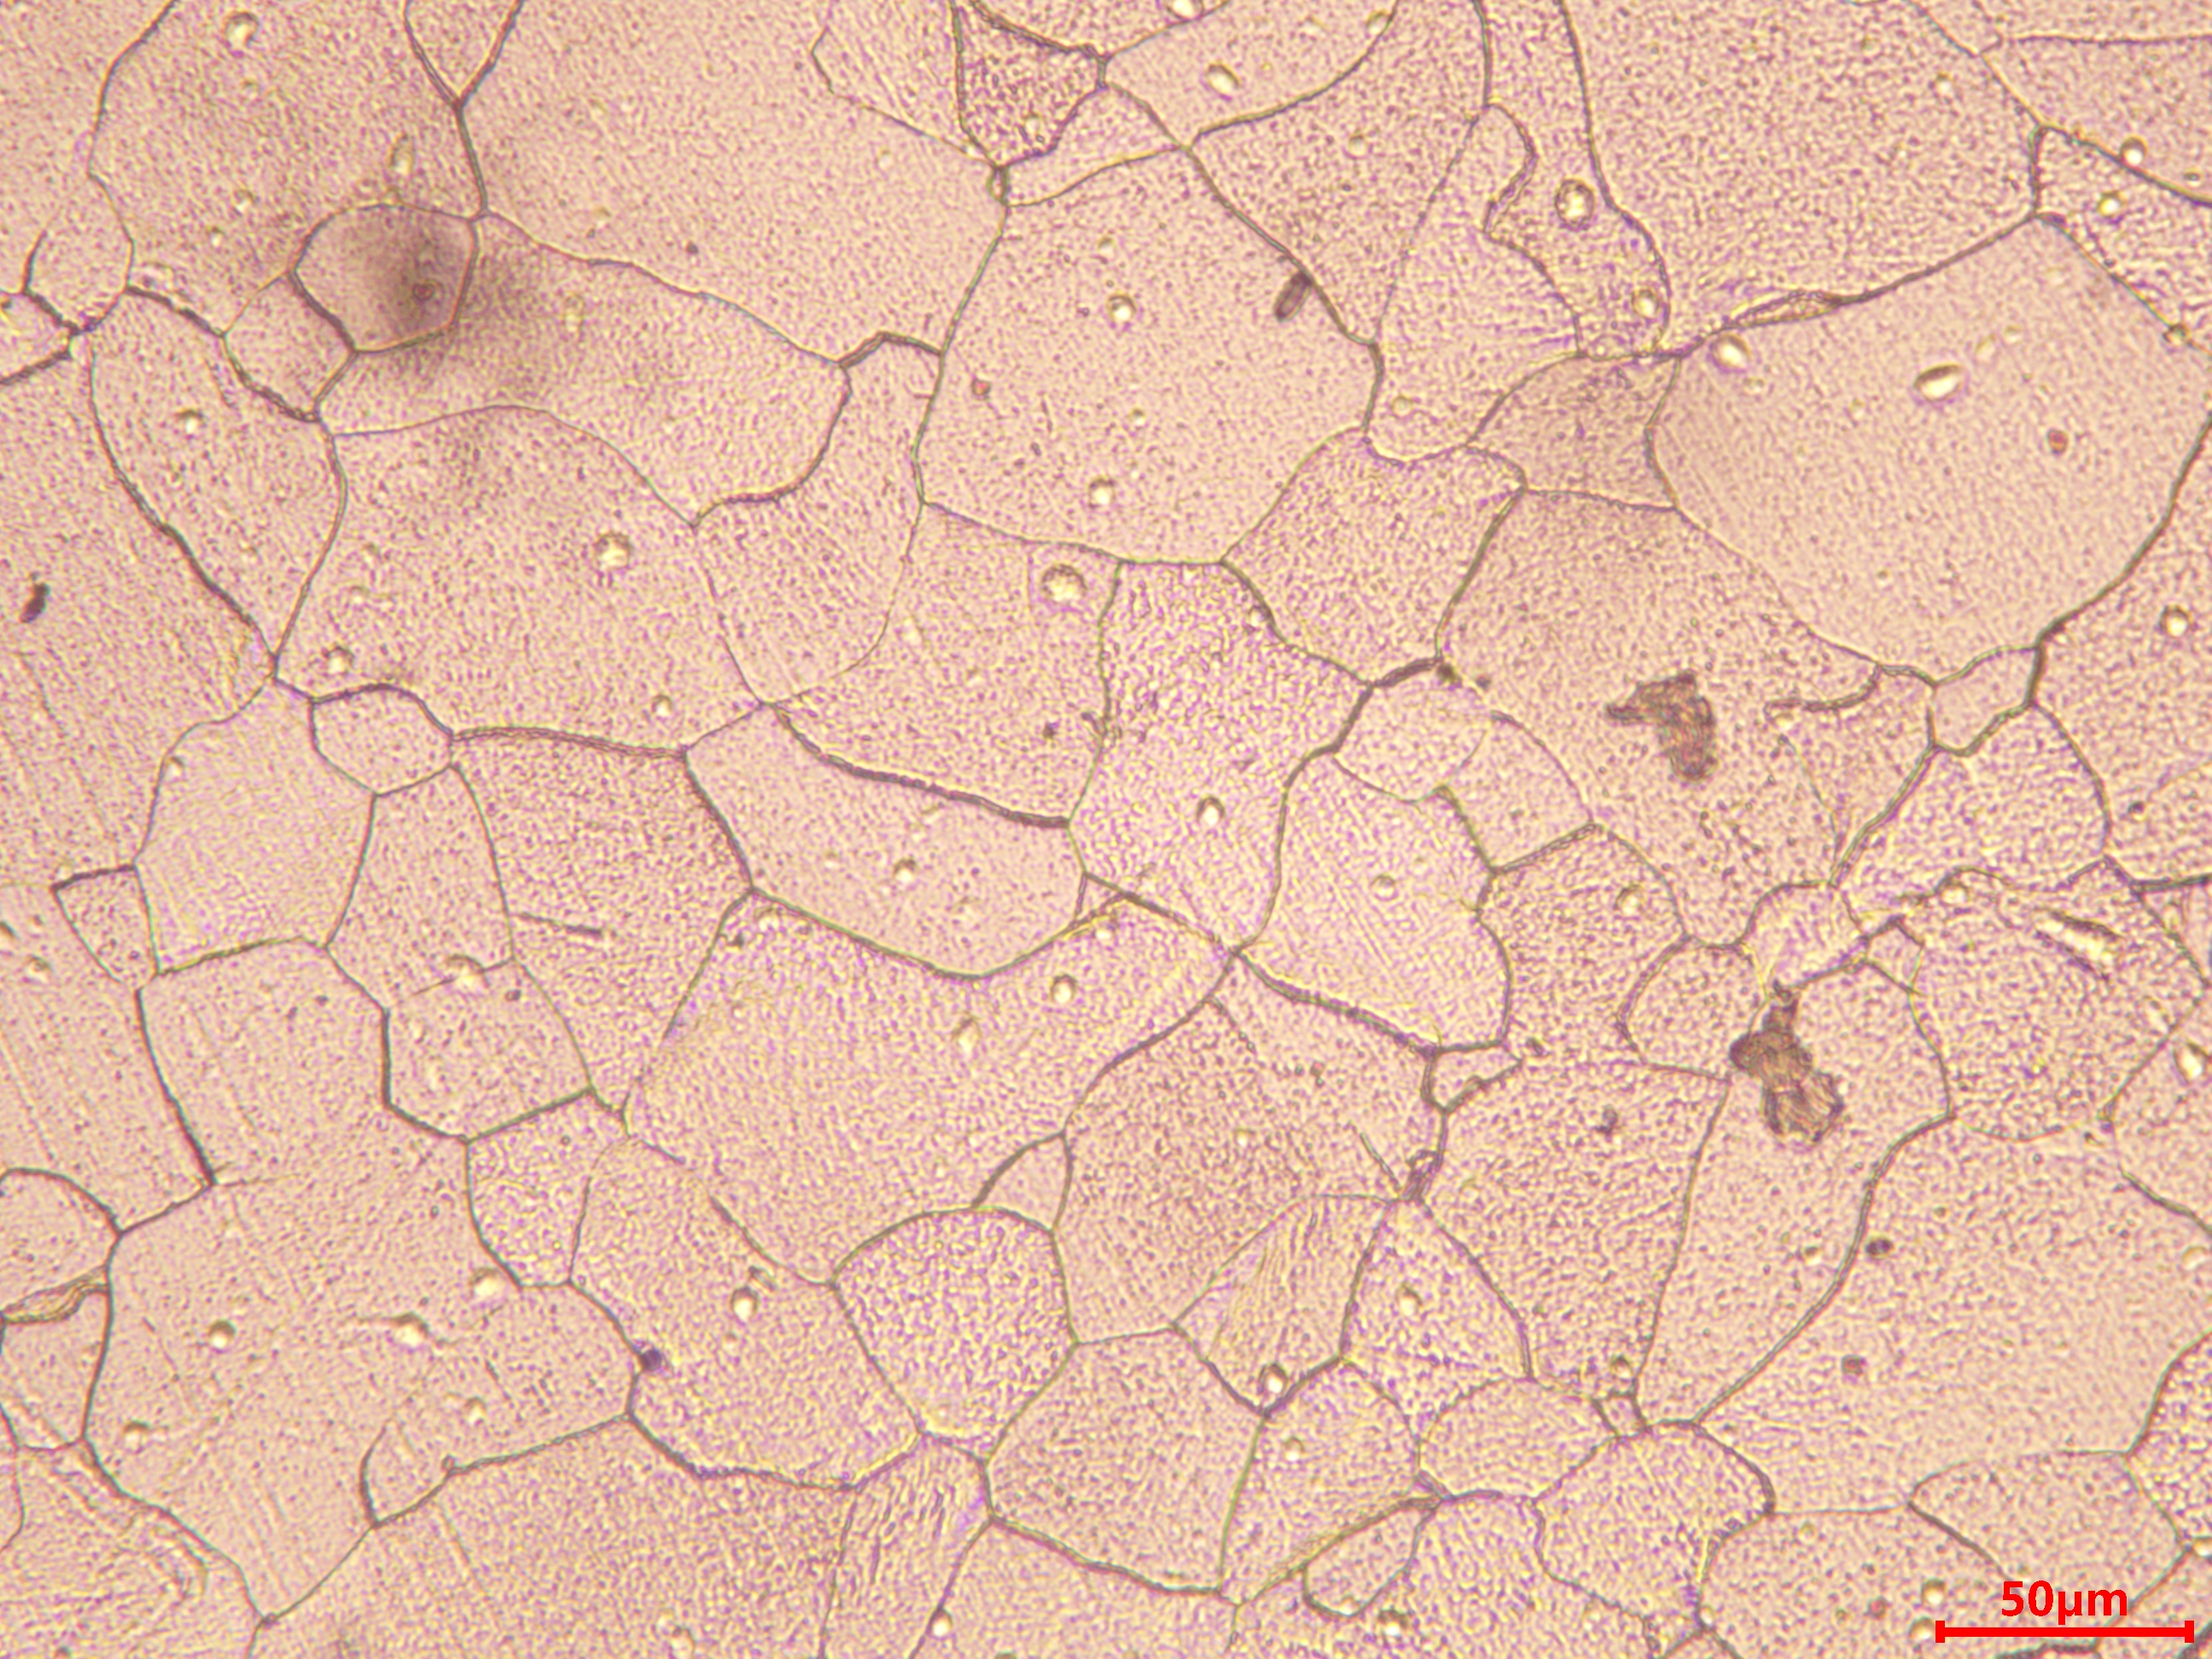
\includegraphics[height=24mm]{img/A1/01_200x.jpg}}\hspace{20pt}
        \subfloat[$500\times{}$]{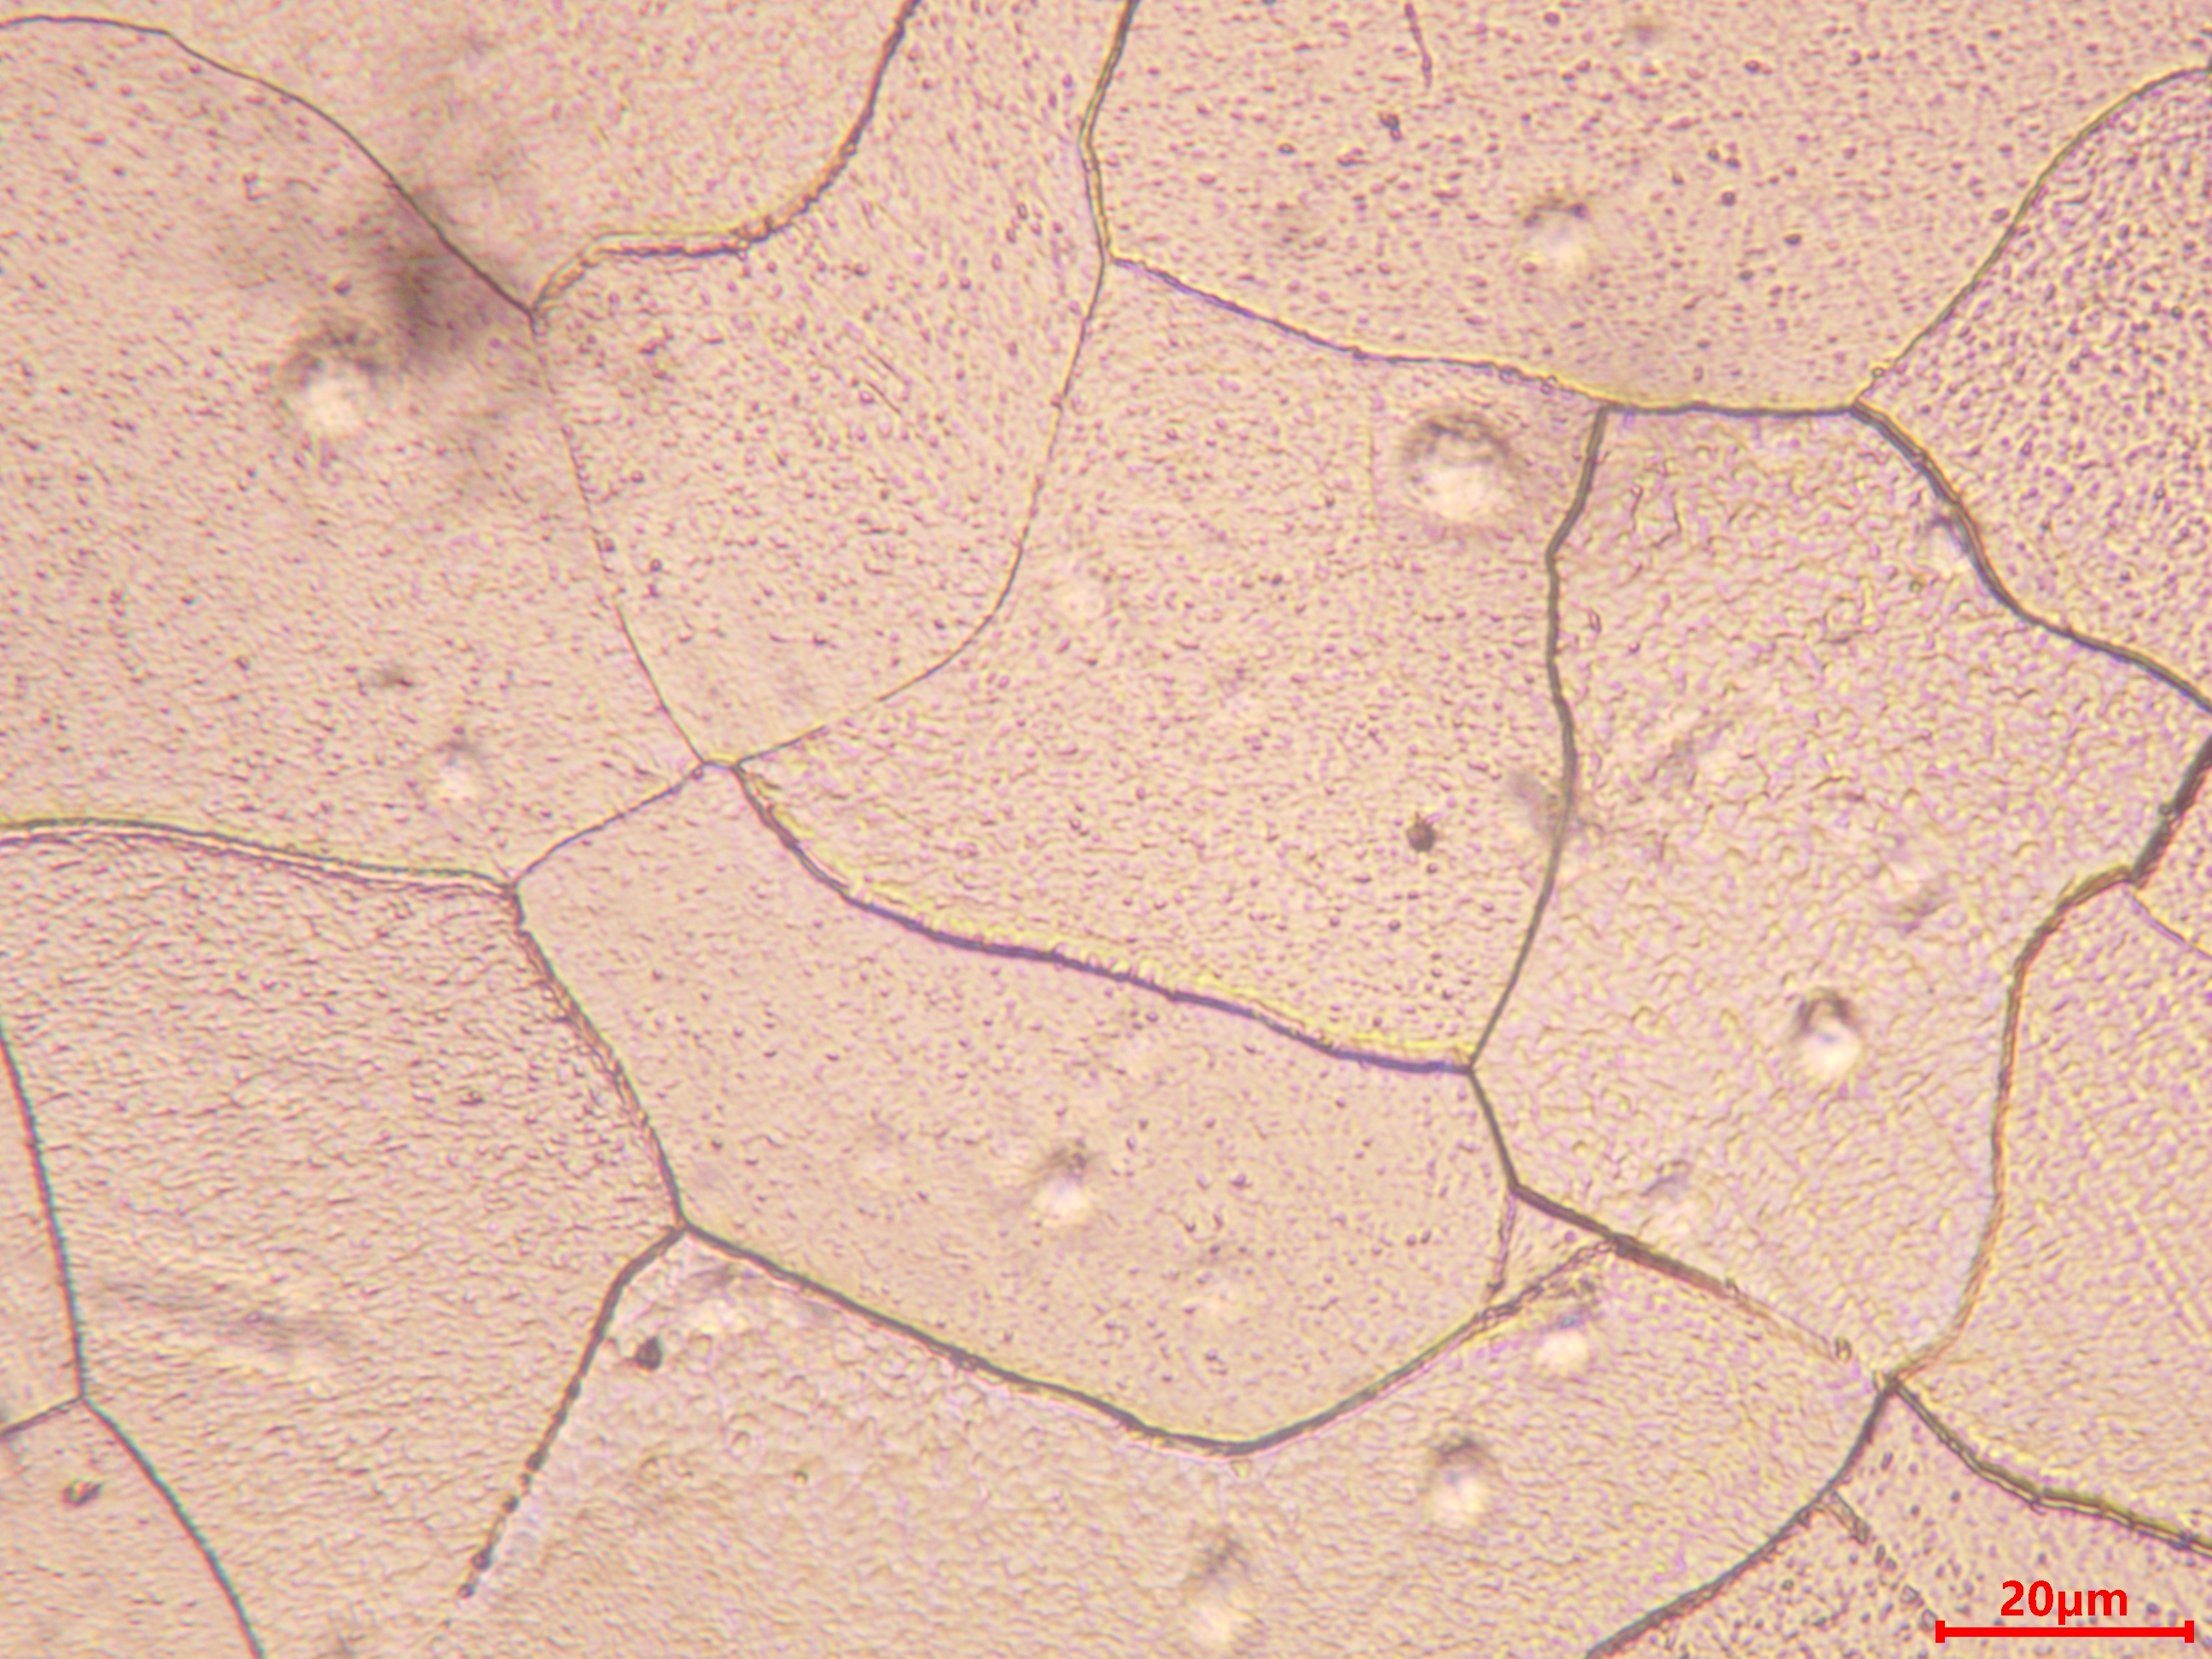
\includegraphics[height=24mm]{img/A1/01_500x.jpg}}\hspace{20pt}
        \subfloat[手绘图]{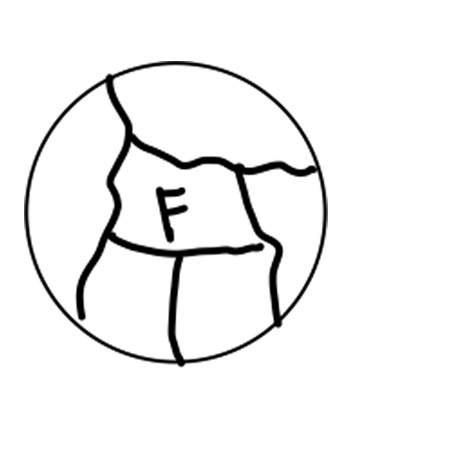
\includegraphics[height=24mm]{img/A1/n1.jpg}}
        \caption{工业纯铁显微组织\label{fig:n1}}
    \end{figure}

    \subsubsection{亚共析钢}
    亚共析钢的含碳量为 $0.0218\%\sim 0.77\%$,室温下的显微组织由白色块状铁素体(F)和珠光体(P)构成。由于珠光体在层片间距较小或者放大倍数较低,珠光体的片层结构未能很好地展现。45 钢的显微组织如\fgref{fig:n2} 所示。
    \begin{figure}[!ht]
        \subfloat[$200\times{}$]{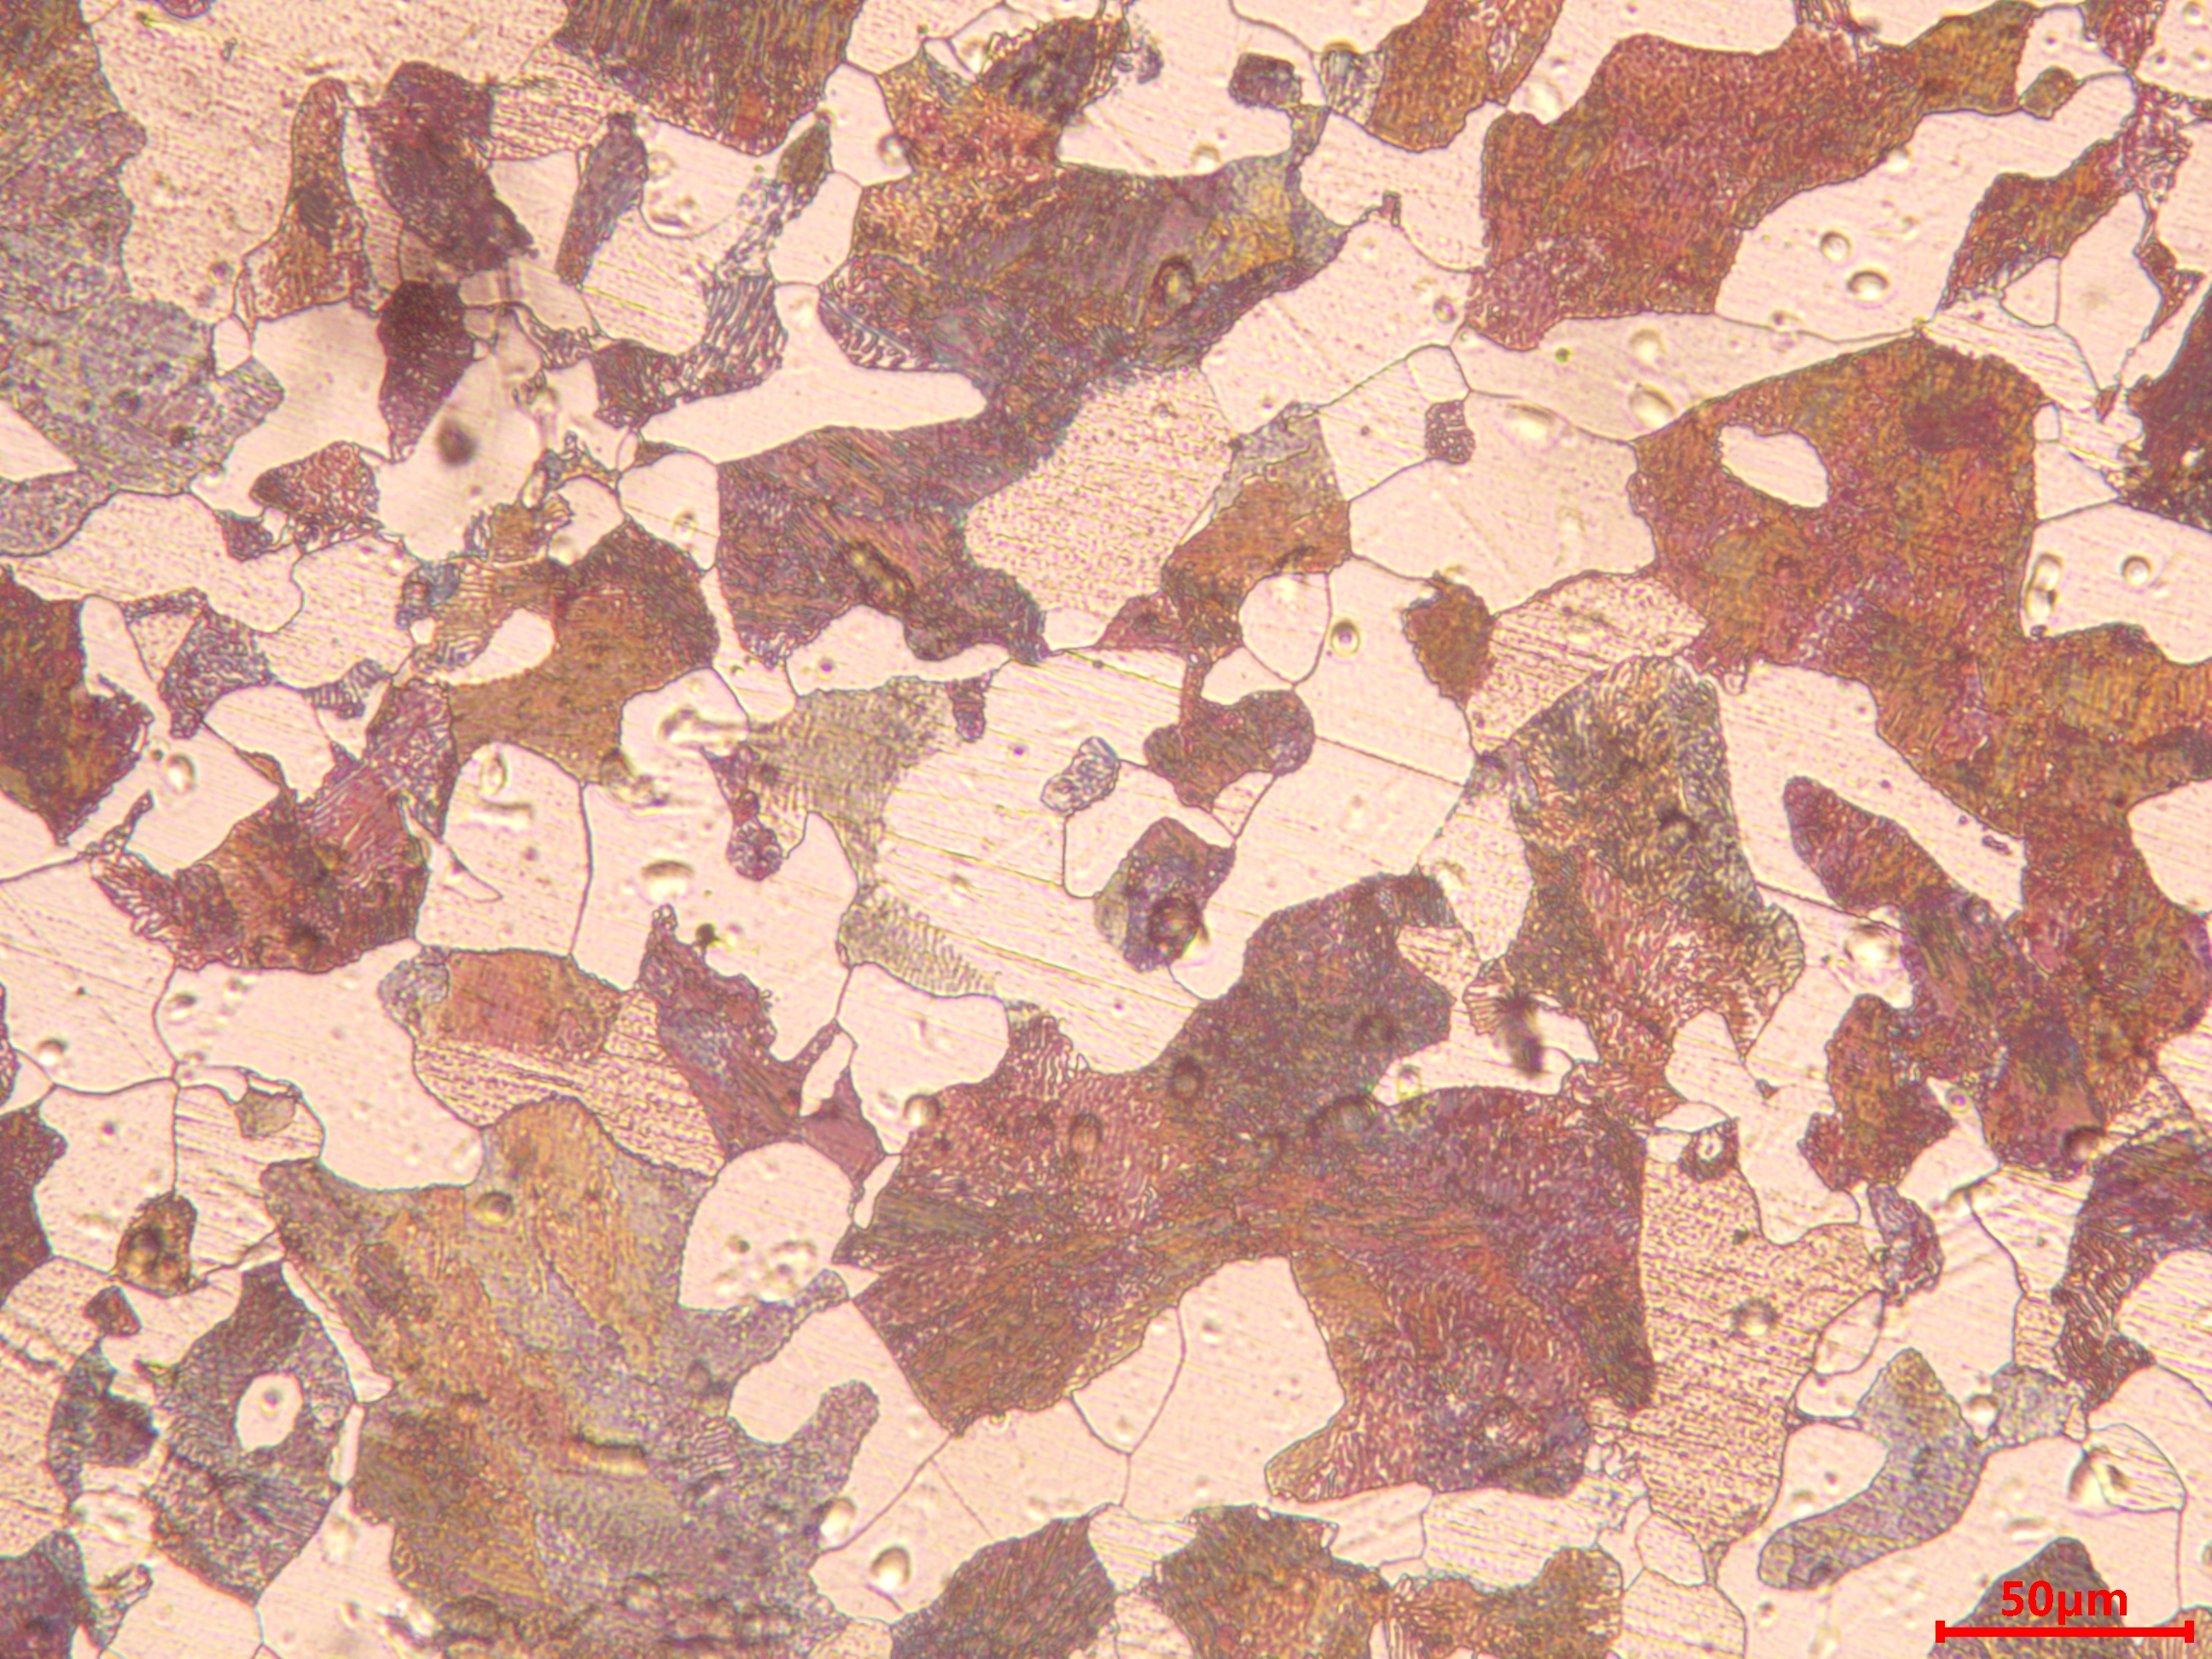
\includegraphics[height=24mm]{img/A1/03_200x.jpg}}\hspace{20pt}
        \subfloat[$500\times{}$]{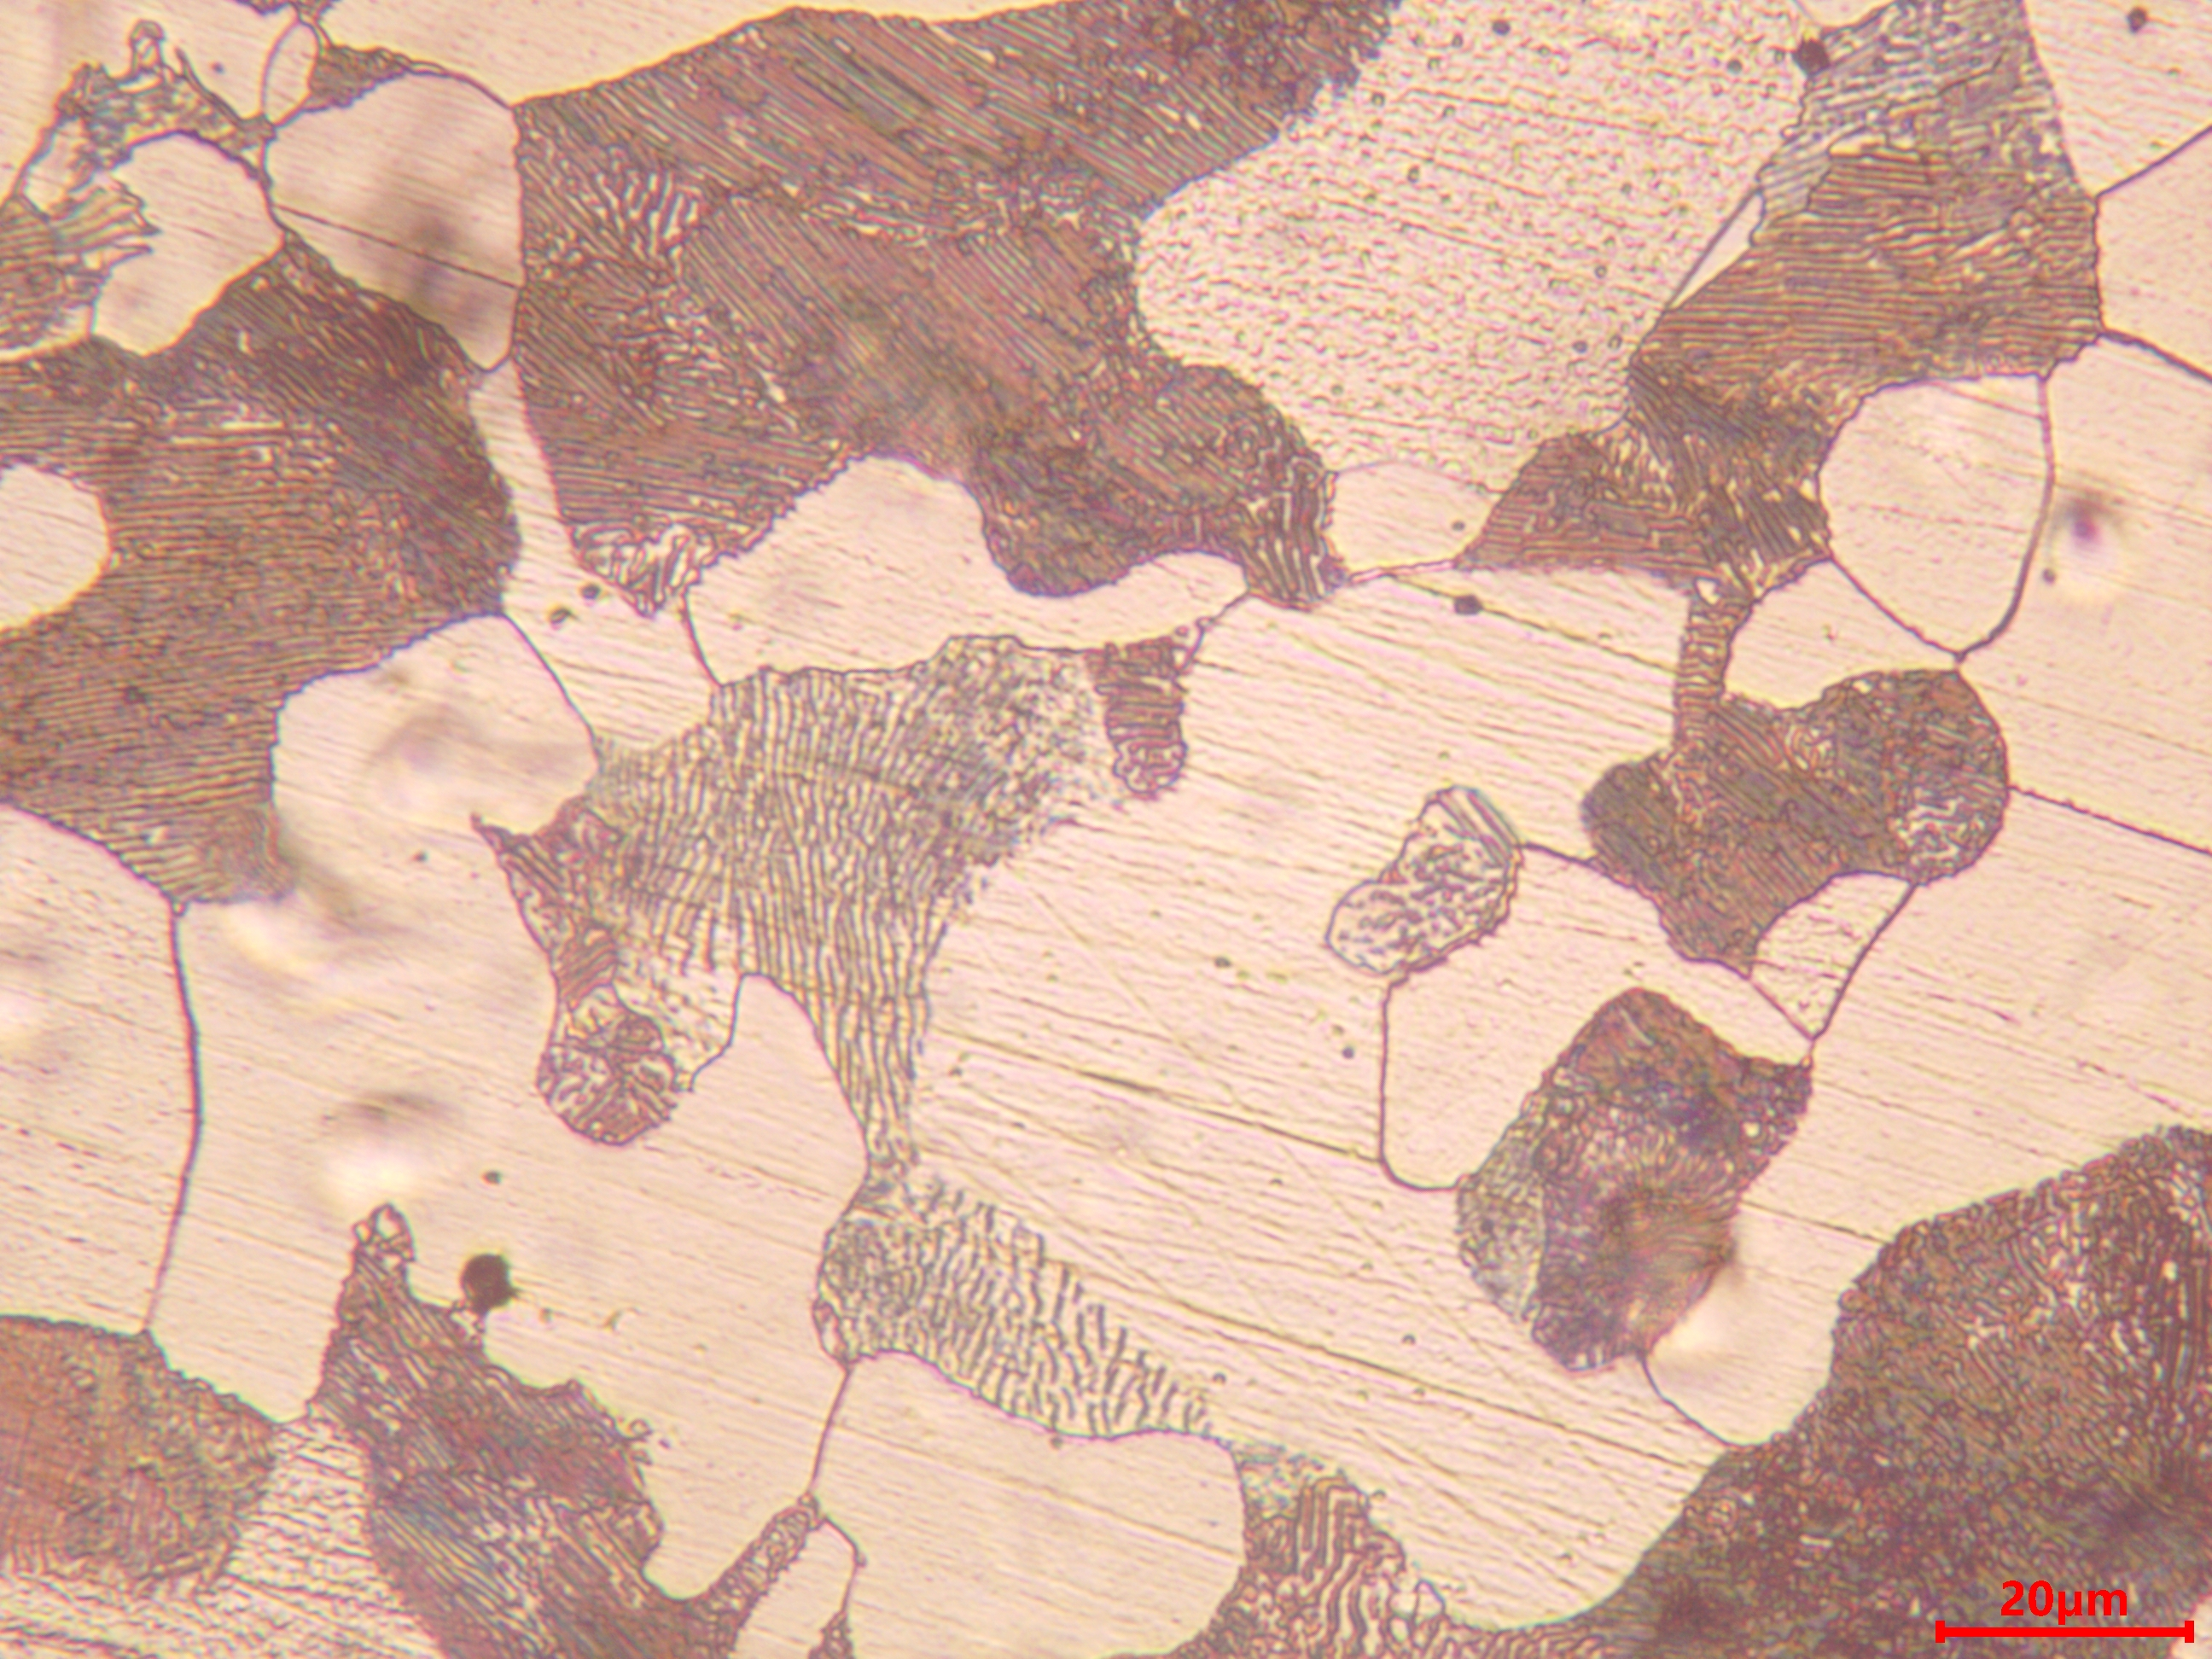
\includegraphics[height=24mm]{img/A1/03_500x.jpg}}\hspace{20pt}
        \subfloat[手绘图]{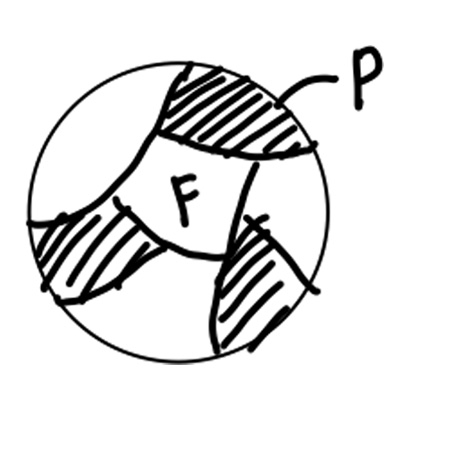
\includegraphics[height=24mm]{img/A1/n2.jpg}}
        \caption{45 钢显微组织\label{fig:n2}}
    \end{figure}

    \subsubsection{共析钢}
    共析钢含碳量为 0.77\%,室温下的显微组织全部由层片状珠光体(P)组织构成,即片状铁素体和渗碳体的机械混合物。根据杠杆定理计算可知珠光体中铁素体与渗碳体的质量比约为 $7.9:1$,因此铁素体厚,渗碳体薄。用硝酸酒精浸蚀后,珠光体中铁素体与渗碳体都呈白亮色,只有相界呈黑色。T8 钢的显微组织如\fgref{fig:n3} 所示。
    \begin{figure}[!ht]
        \subfloat[$200\times{}$]{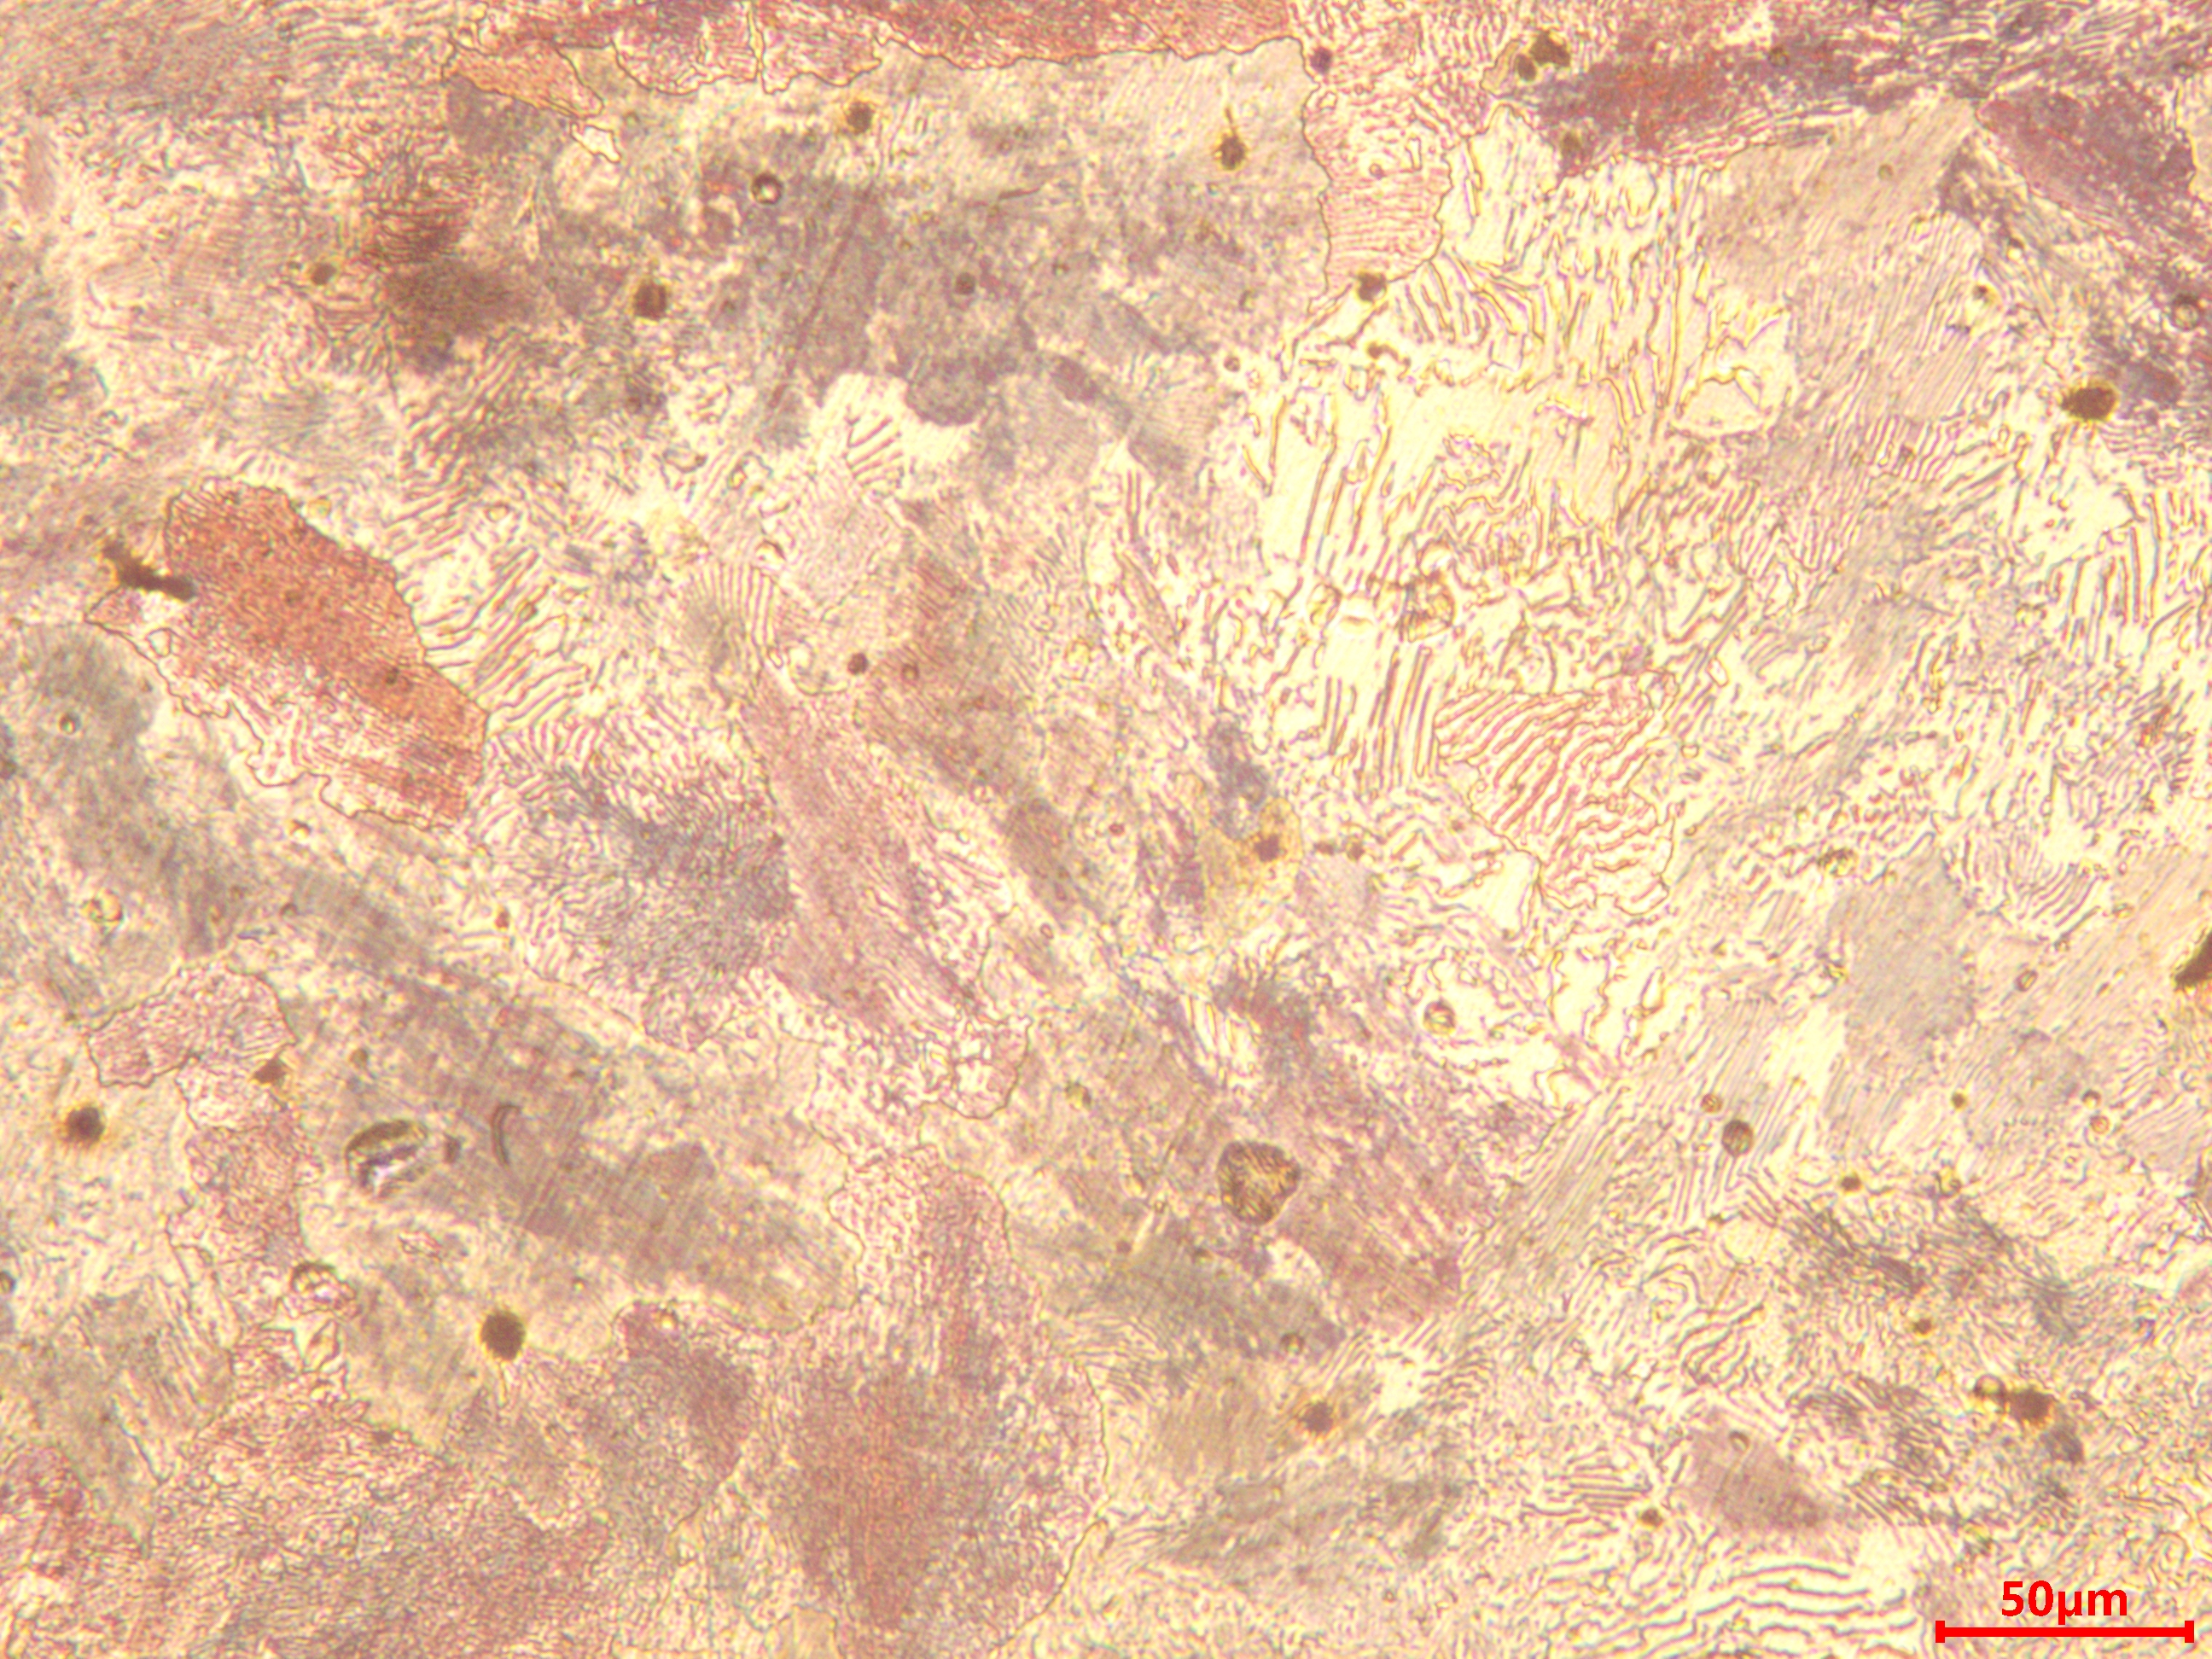
\includegraphics[height=24mm]{img/A1/05_200x.jpg}}\hspace{20pt}
        \subfloat[$500\times{}$]{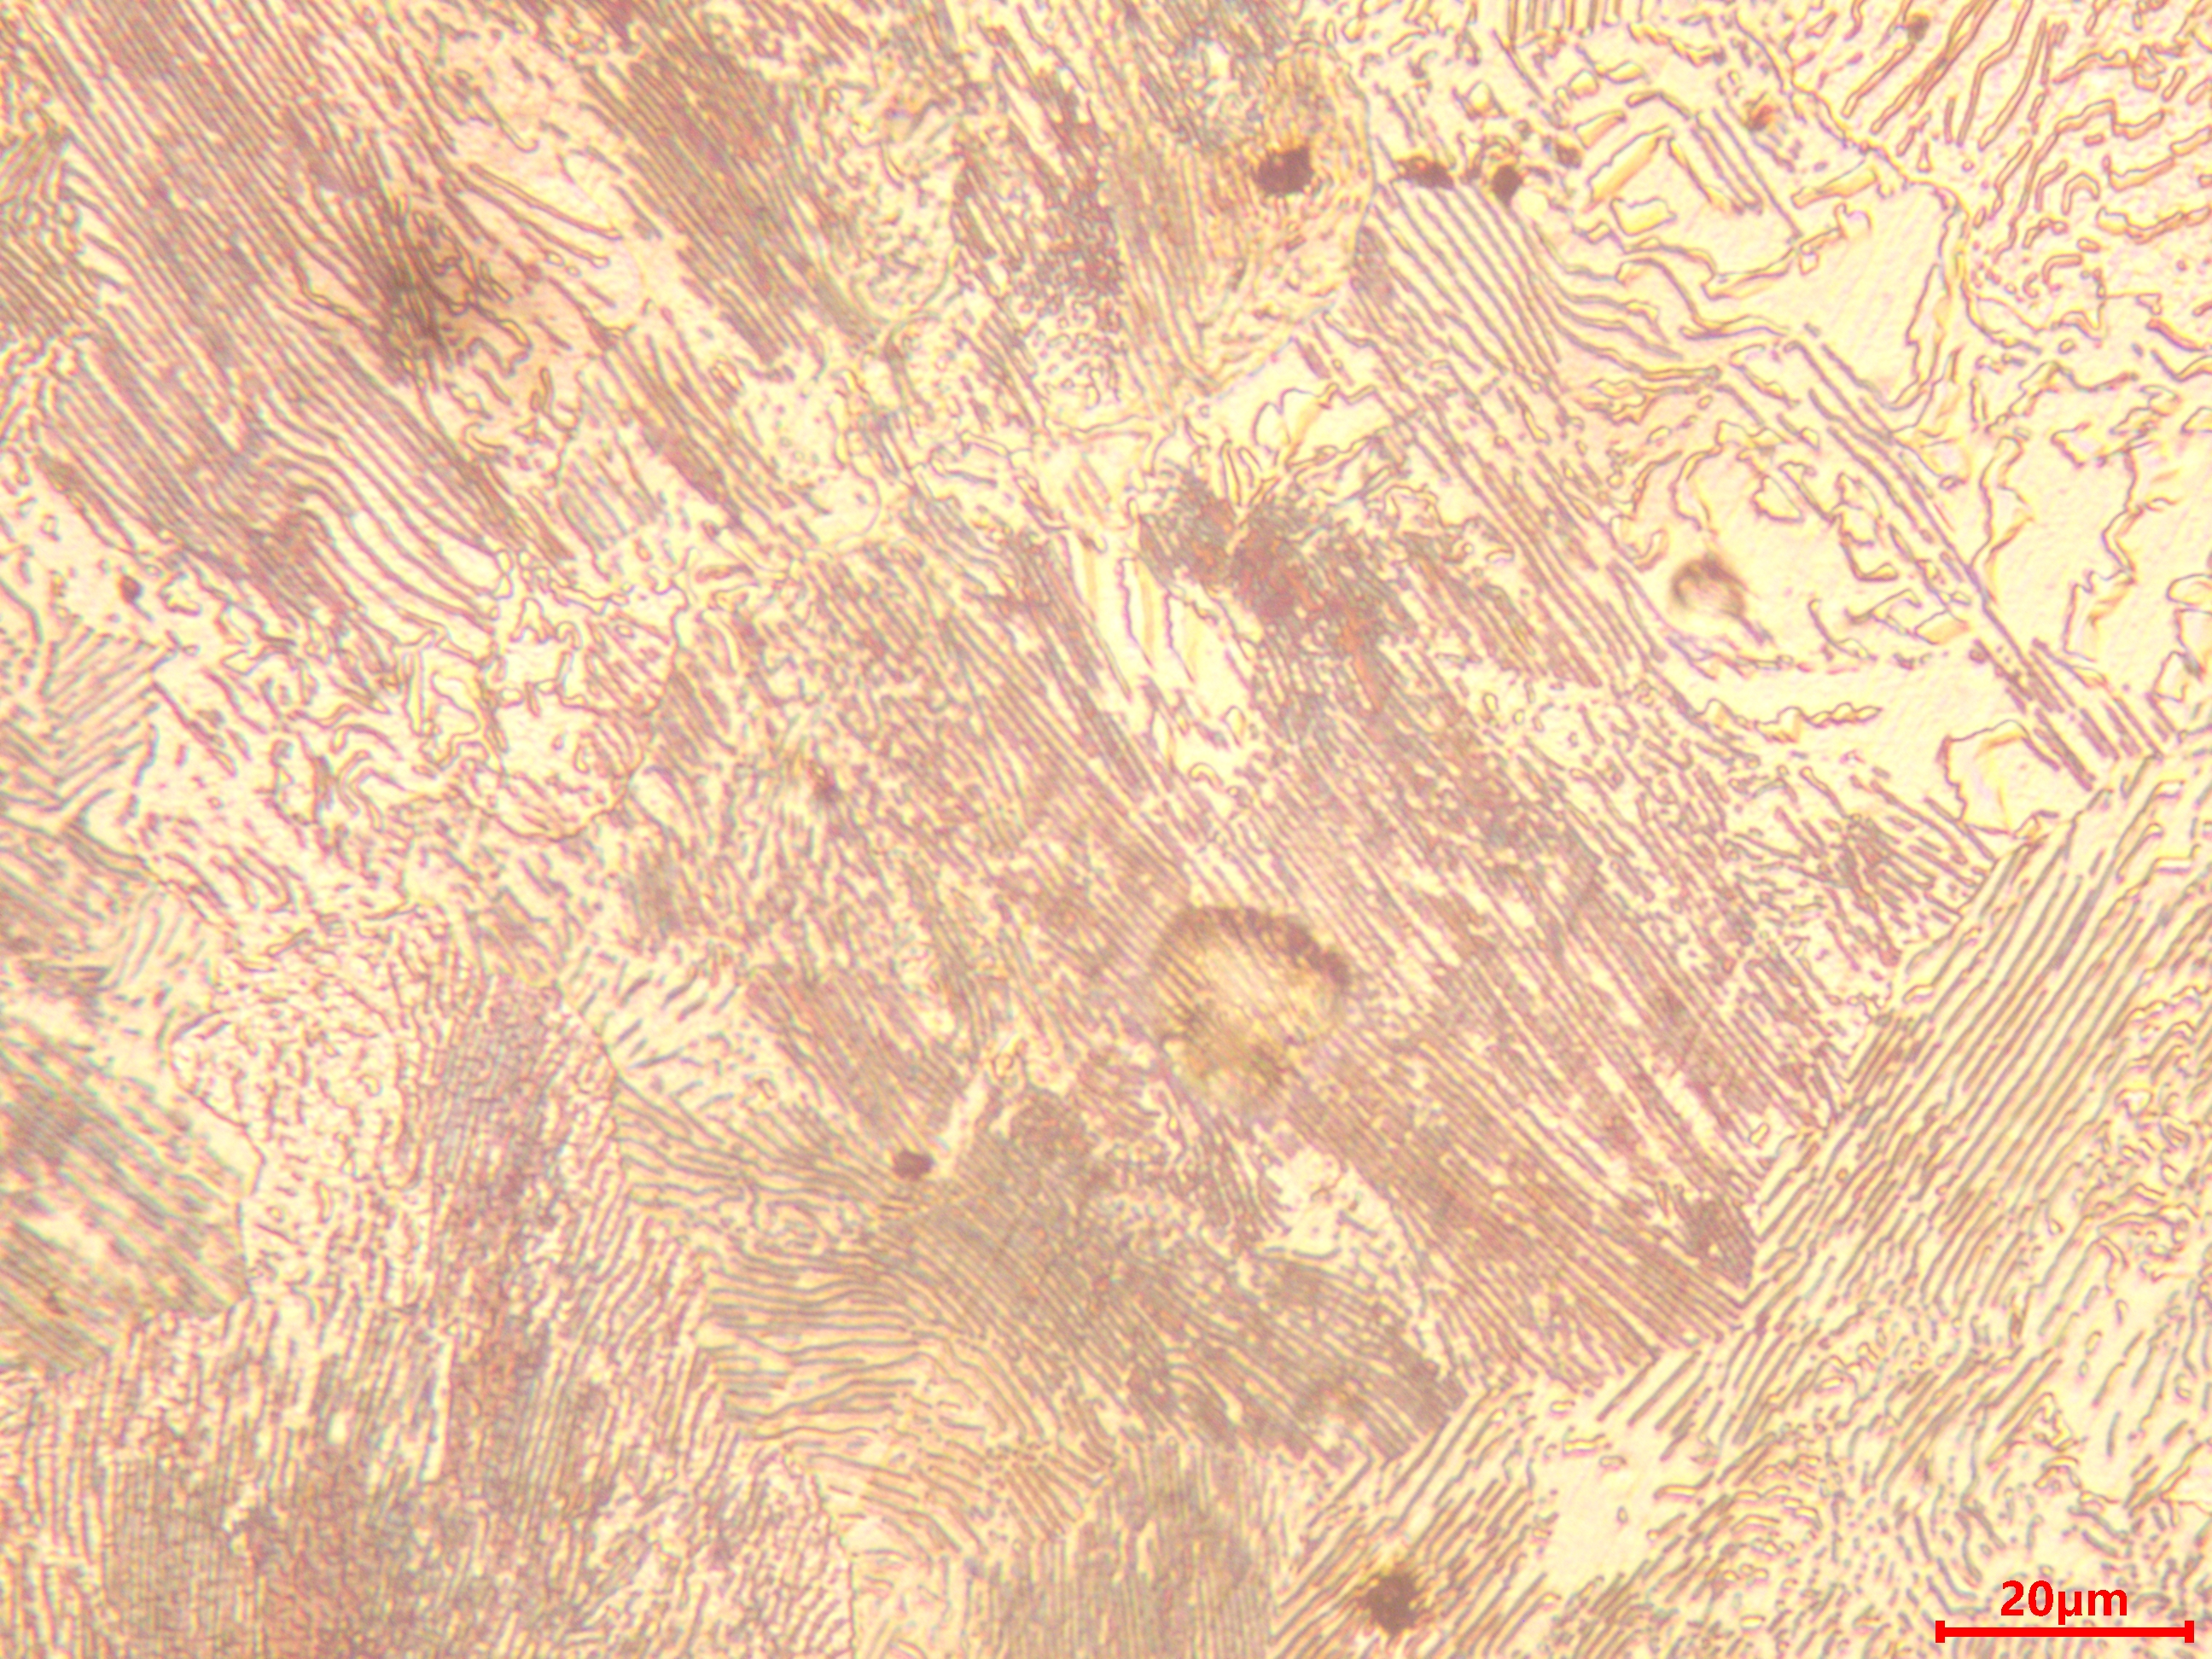
\includegraphics[height=24mm]{img/A1/05_500x.jpg}}\hspace{20pt}
        \subfloat[手绘图]{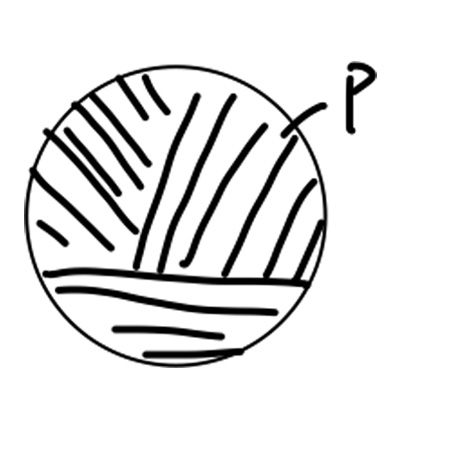
\includegraphics[height=24mm]{img/A1/n3.jpg}}
        \caption{T8 钢显微组织\label{fig:n3}}
    \end{figure}

    \subsubsection{过共析钢}
    过共析钢含碳量为 $0.77\%\sim 2.11\%$,室温下的显微组织由白亮色网状二次渗碳体和层片状珠光体(P)构成。随着钢中含碳量增加,二次渗碳体数量也增加。用硝酸酒精浸蚀后,二次渗碳体呈亮白色网分布在珠光体的周围,如\fgref{fig:n4} 所示。
    \begin{figure}[!ht]
        \subfloat[$200\times{}$]{\includegraphics[height=24mm]{img/A1/06_200x.jpg}}\hspace{20pt}
        \subfloat[$500\times{}$]{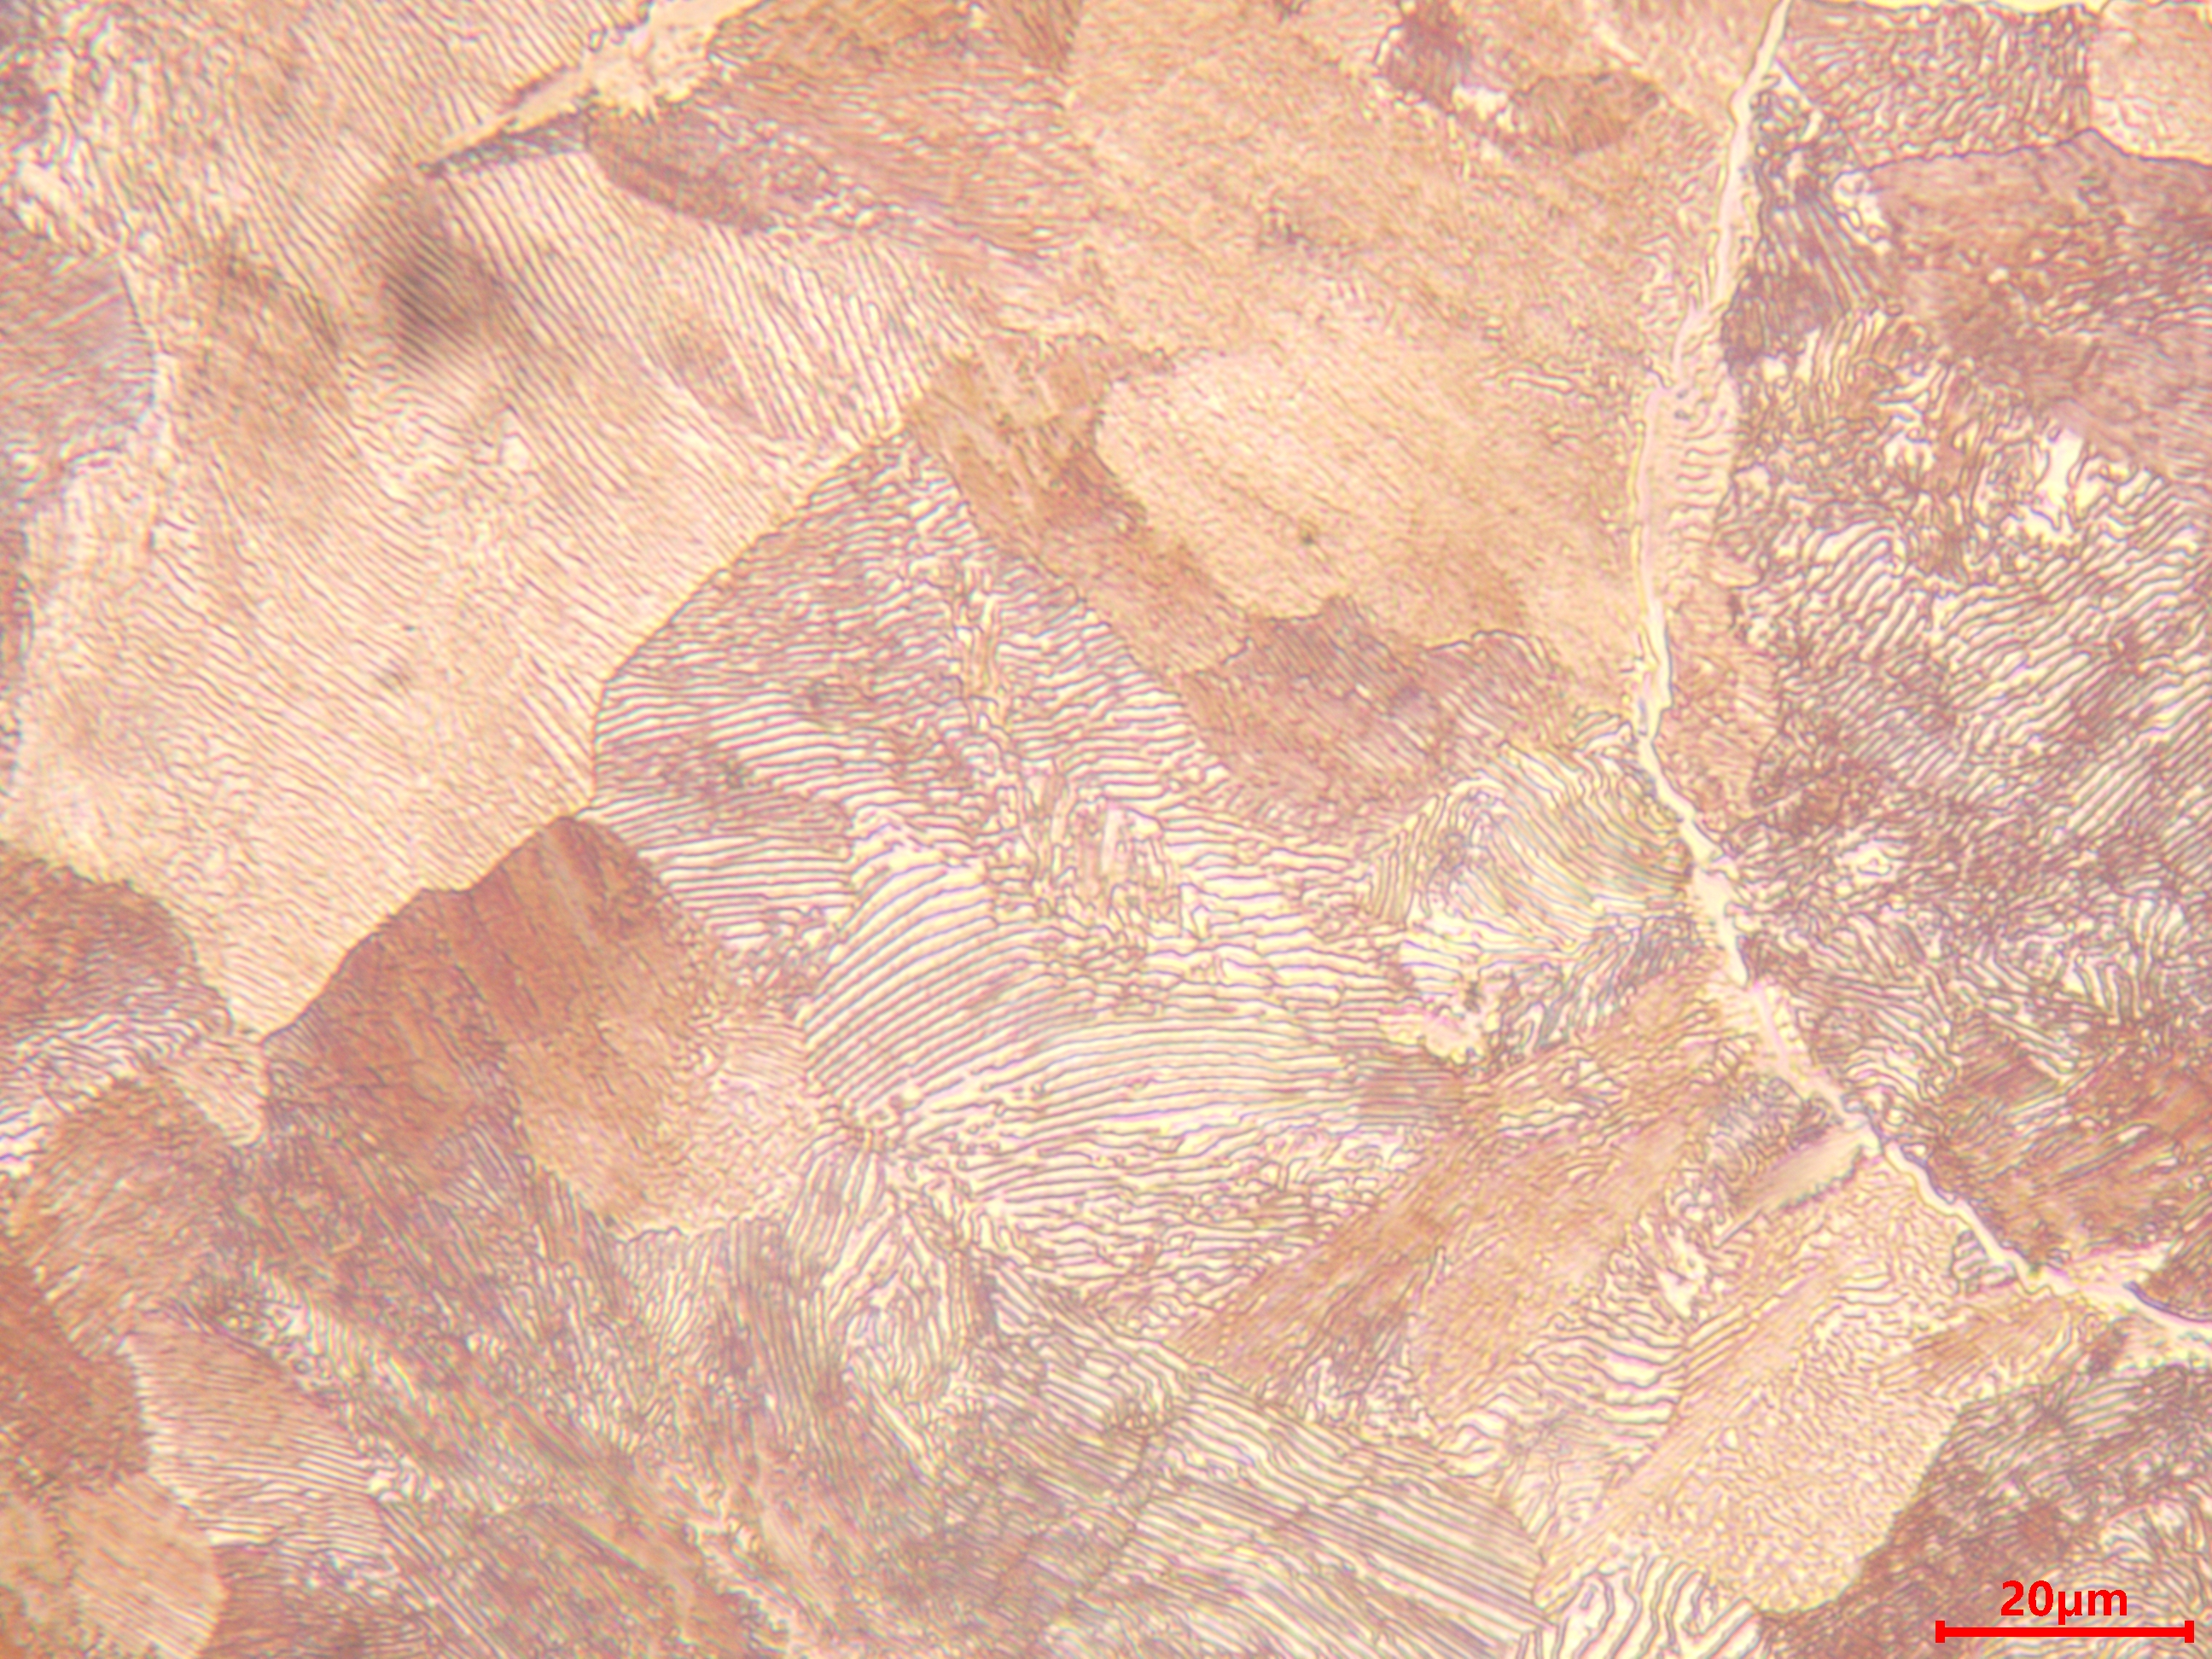
\includegraphics[height=24mm]{img/A1/06_500x.jpg}}\hspace{20pt}
        \subfloat[手绘图]{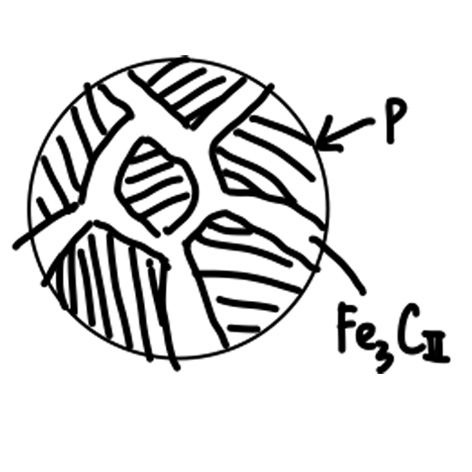
\includegraphics[height=24mm]{img/A1/n4.jpg}}
        \caption{T12 钢显微组织\label{fig:n4}}
    \end{figure}

    \subsubsection{亚共晶白口铸铁}
    亚共晶白口铸铁含碳量为 $2.11\%\sim 4.3\%$,室温下的显微组织由黑色树枝装珠光体(P)、二次渗碳体 $\text{Fe}_3\text{C}_\text{II}$ 和豹皮状低温莱氏体 $\text{L}_\text{d}^{'}$ 构成。二次渗碳体在珠光体周围析出,与 $\text{L}_\text{d}^{'}$ 中的渗碳体连在一起难以分辨,如\fgref{fig:n5} 所示。
    \begin{figure}[!ht]
        \subfloat[$200\times{}$]{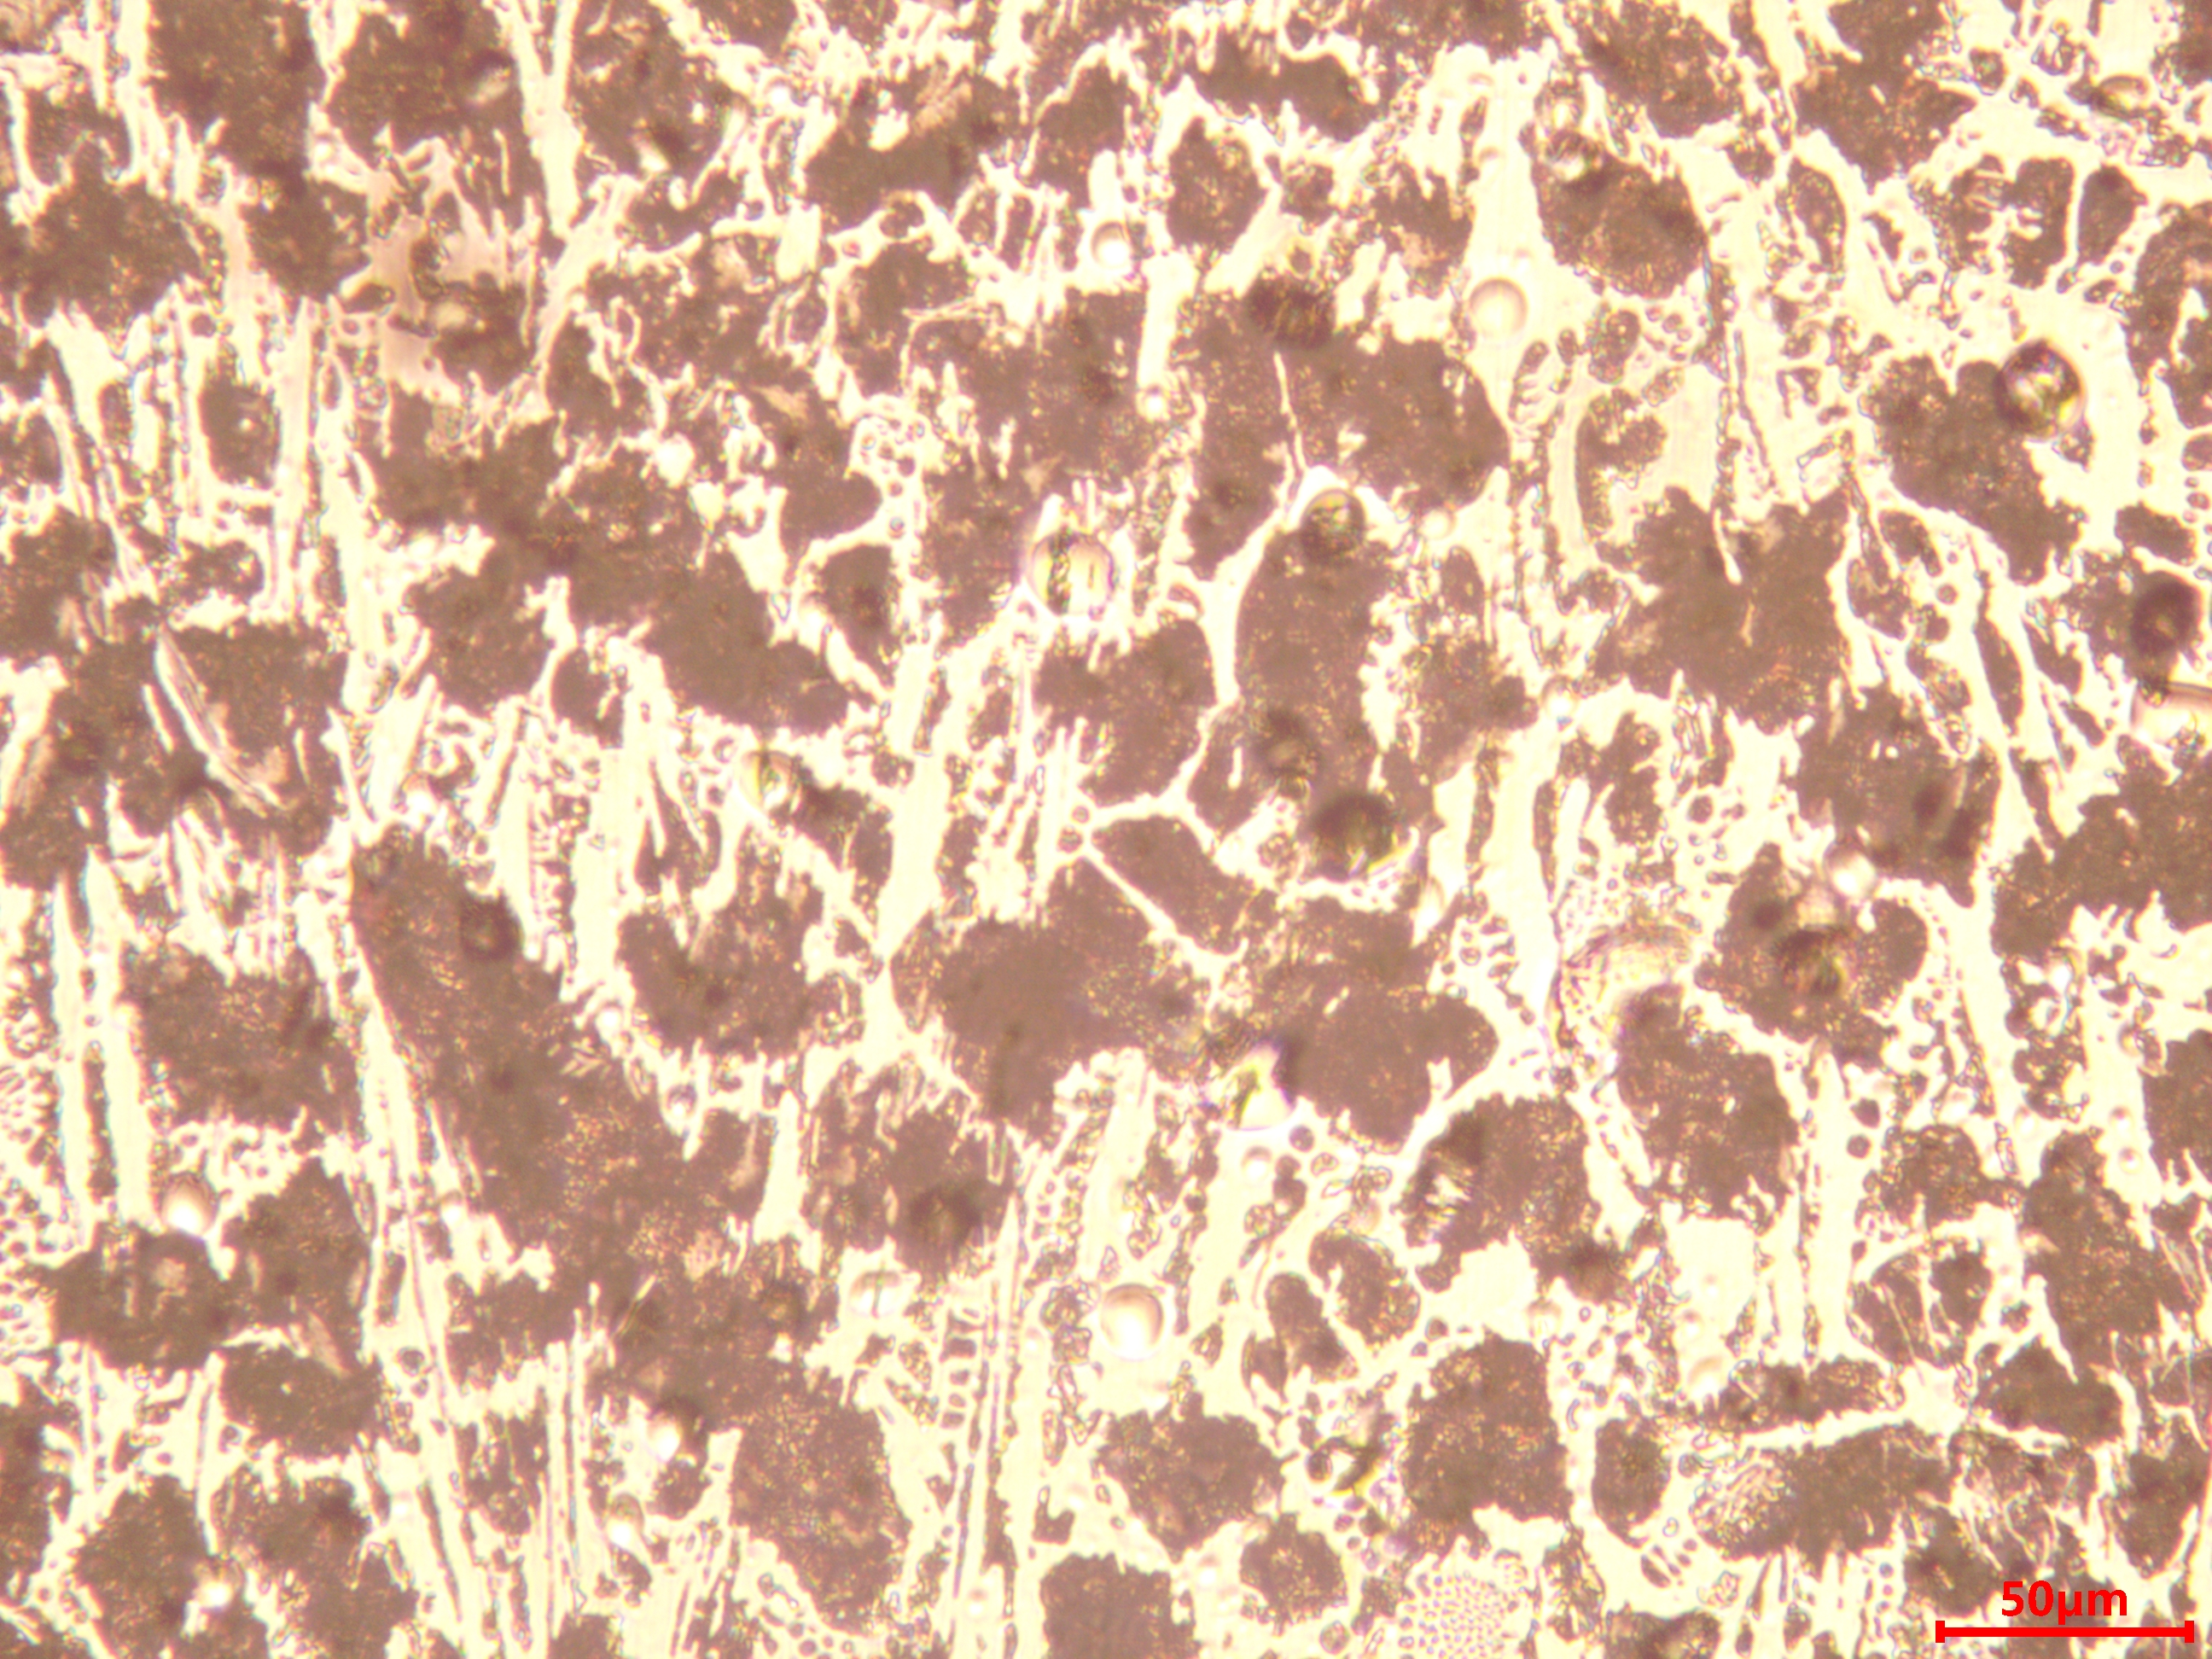
\includegraphics[height=24mm]{img/A1/08_200x.jpg}}\hspace{20pt}
        \subfloat[$500\times{}$]{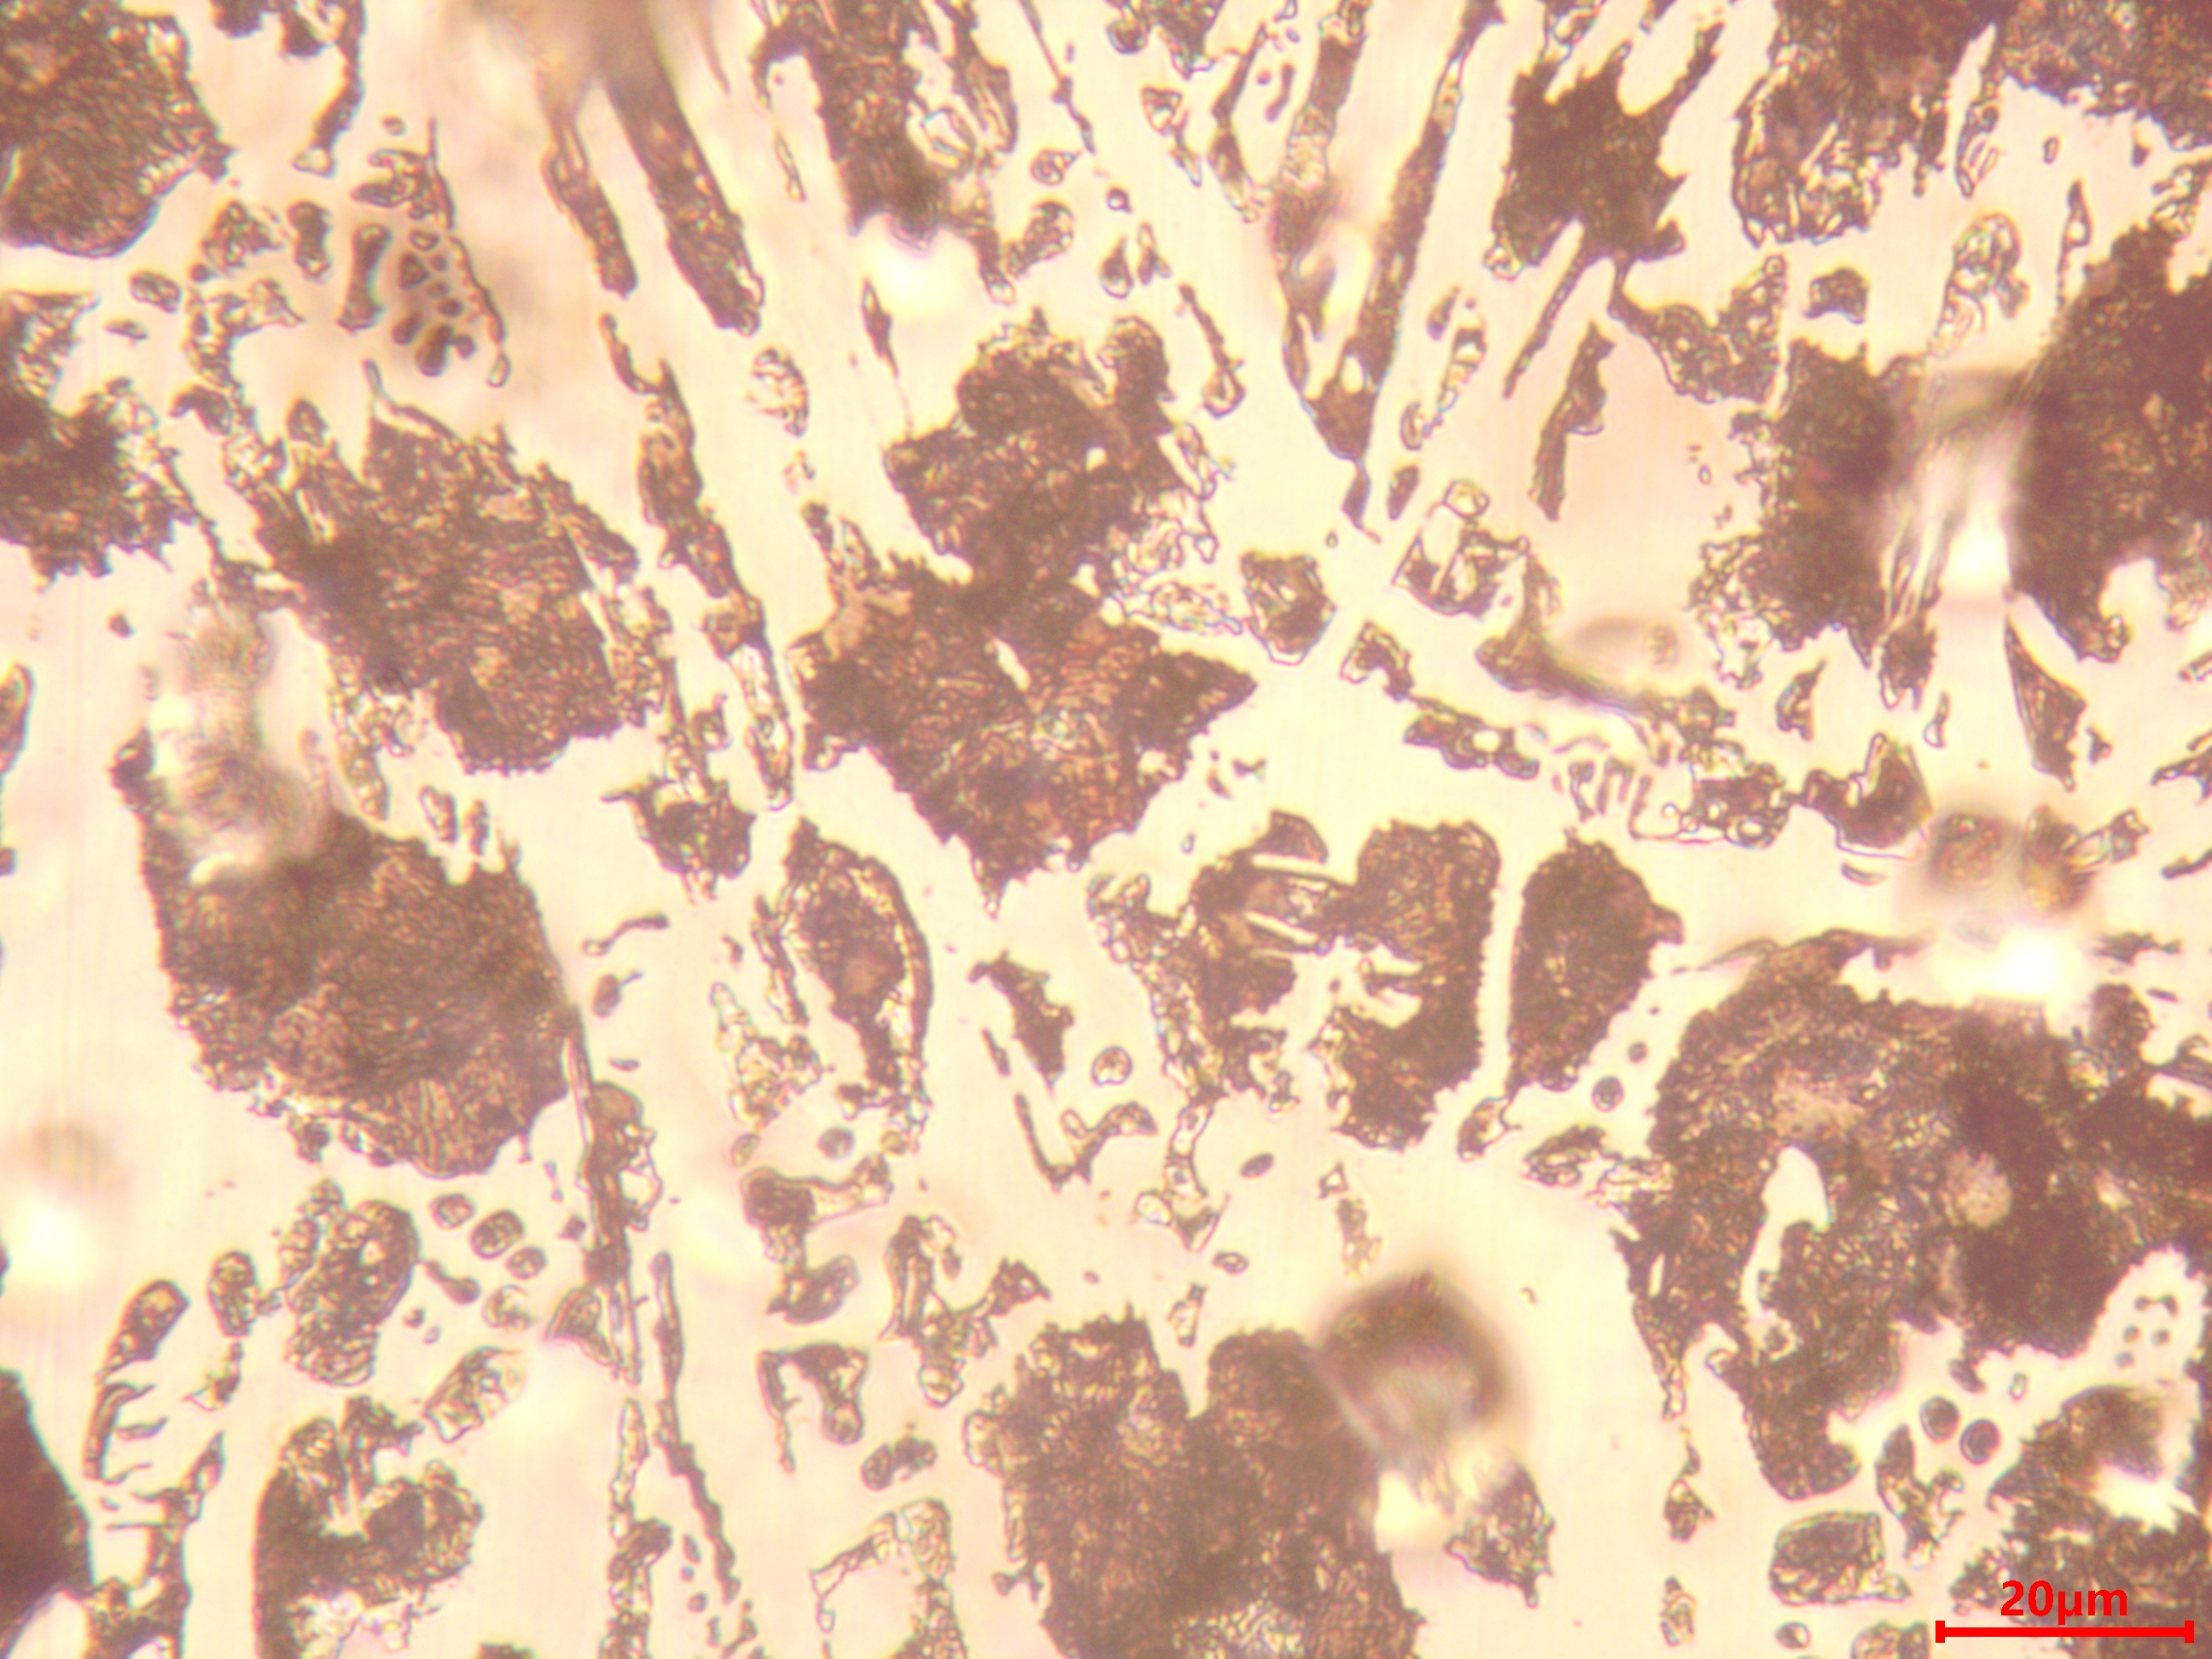
\includegraphics[height=24mm]{img/A1/08_500x.jpg}}\hspace{20pt}
        \subfloat[手绘图]{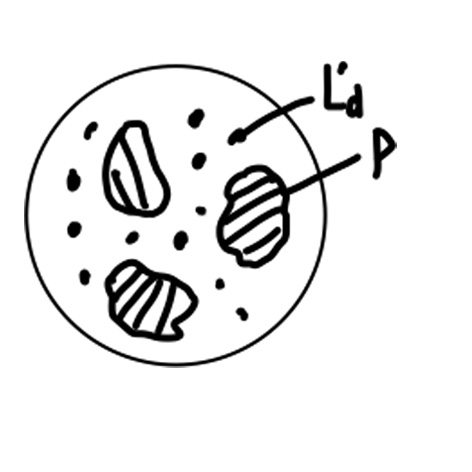
\includegraphics[height=24mm]{img/A1/n5.jpg}}
        \caption{亚共晶白口铸铁显微组织\label{fig:n5}}
    \end{figure}

    \subsubsection{共晶白口铸铁}
    共晶白口铸铁含碳量为 4.3\%,室温下的显微组织由豹皮状低温莱氏体 $\text{L}_\text{d}^{'}$ 构成,其中的白色基体为共晶渗碳体,黑色粒状或棒状组织为珠光体,珠光体的片层状无法分辨而成黑色,如\fgref{fig:n6} 所示。低温莱氏体 $\text{L}_\text{d}^{'}$ 是珠光体和渗碳体组成的机械混合物。
    \begin{figure}[!ht]
        \subfloat[$200\times{}$]{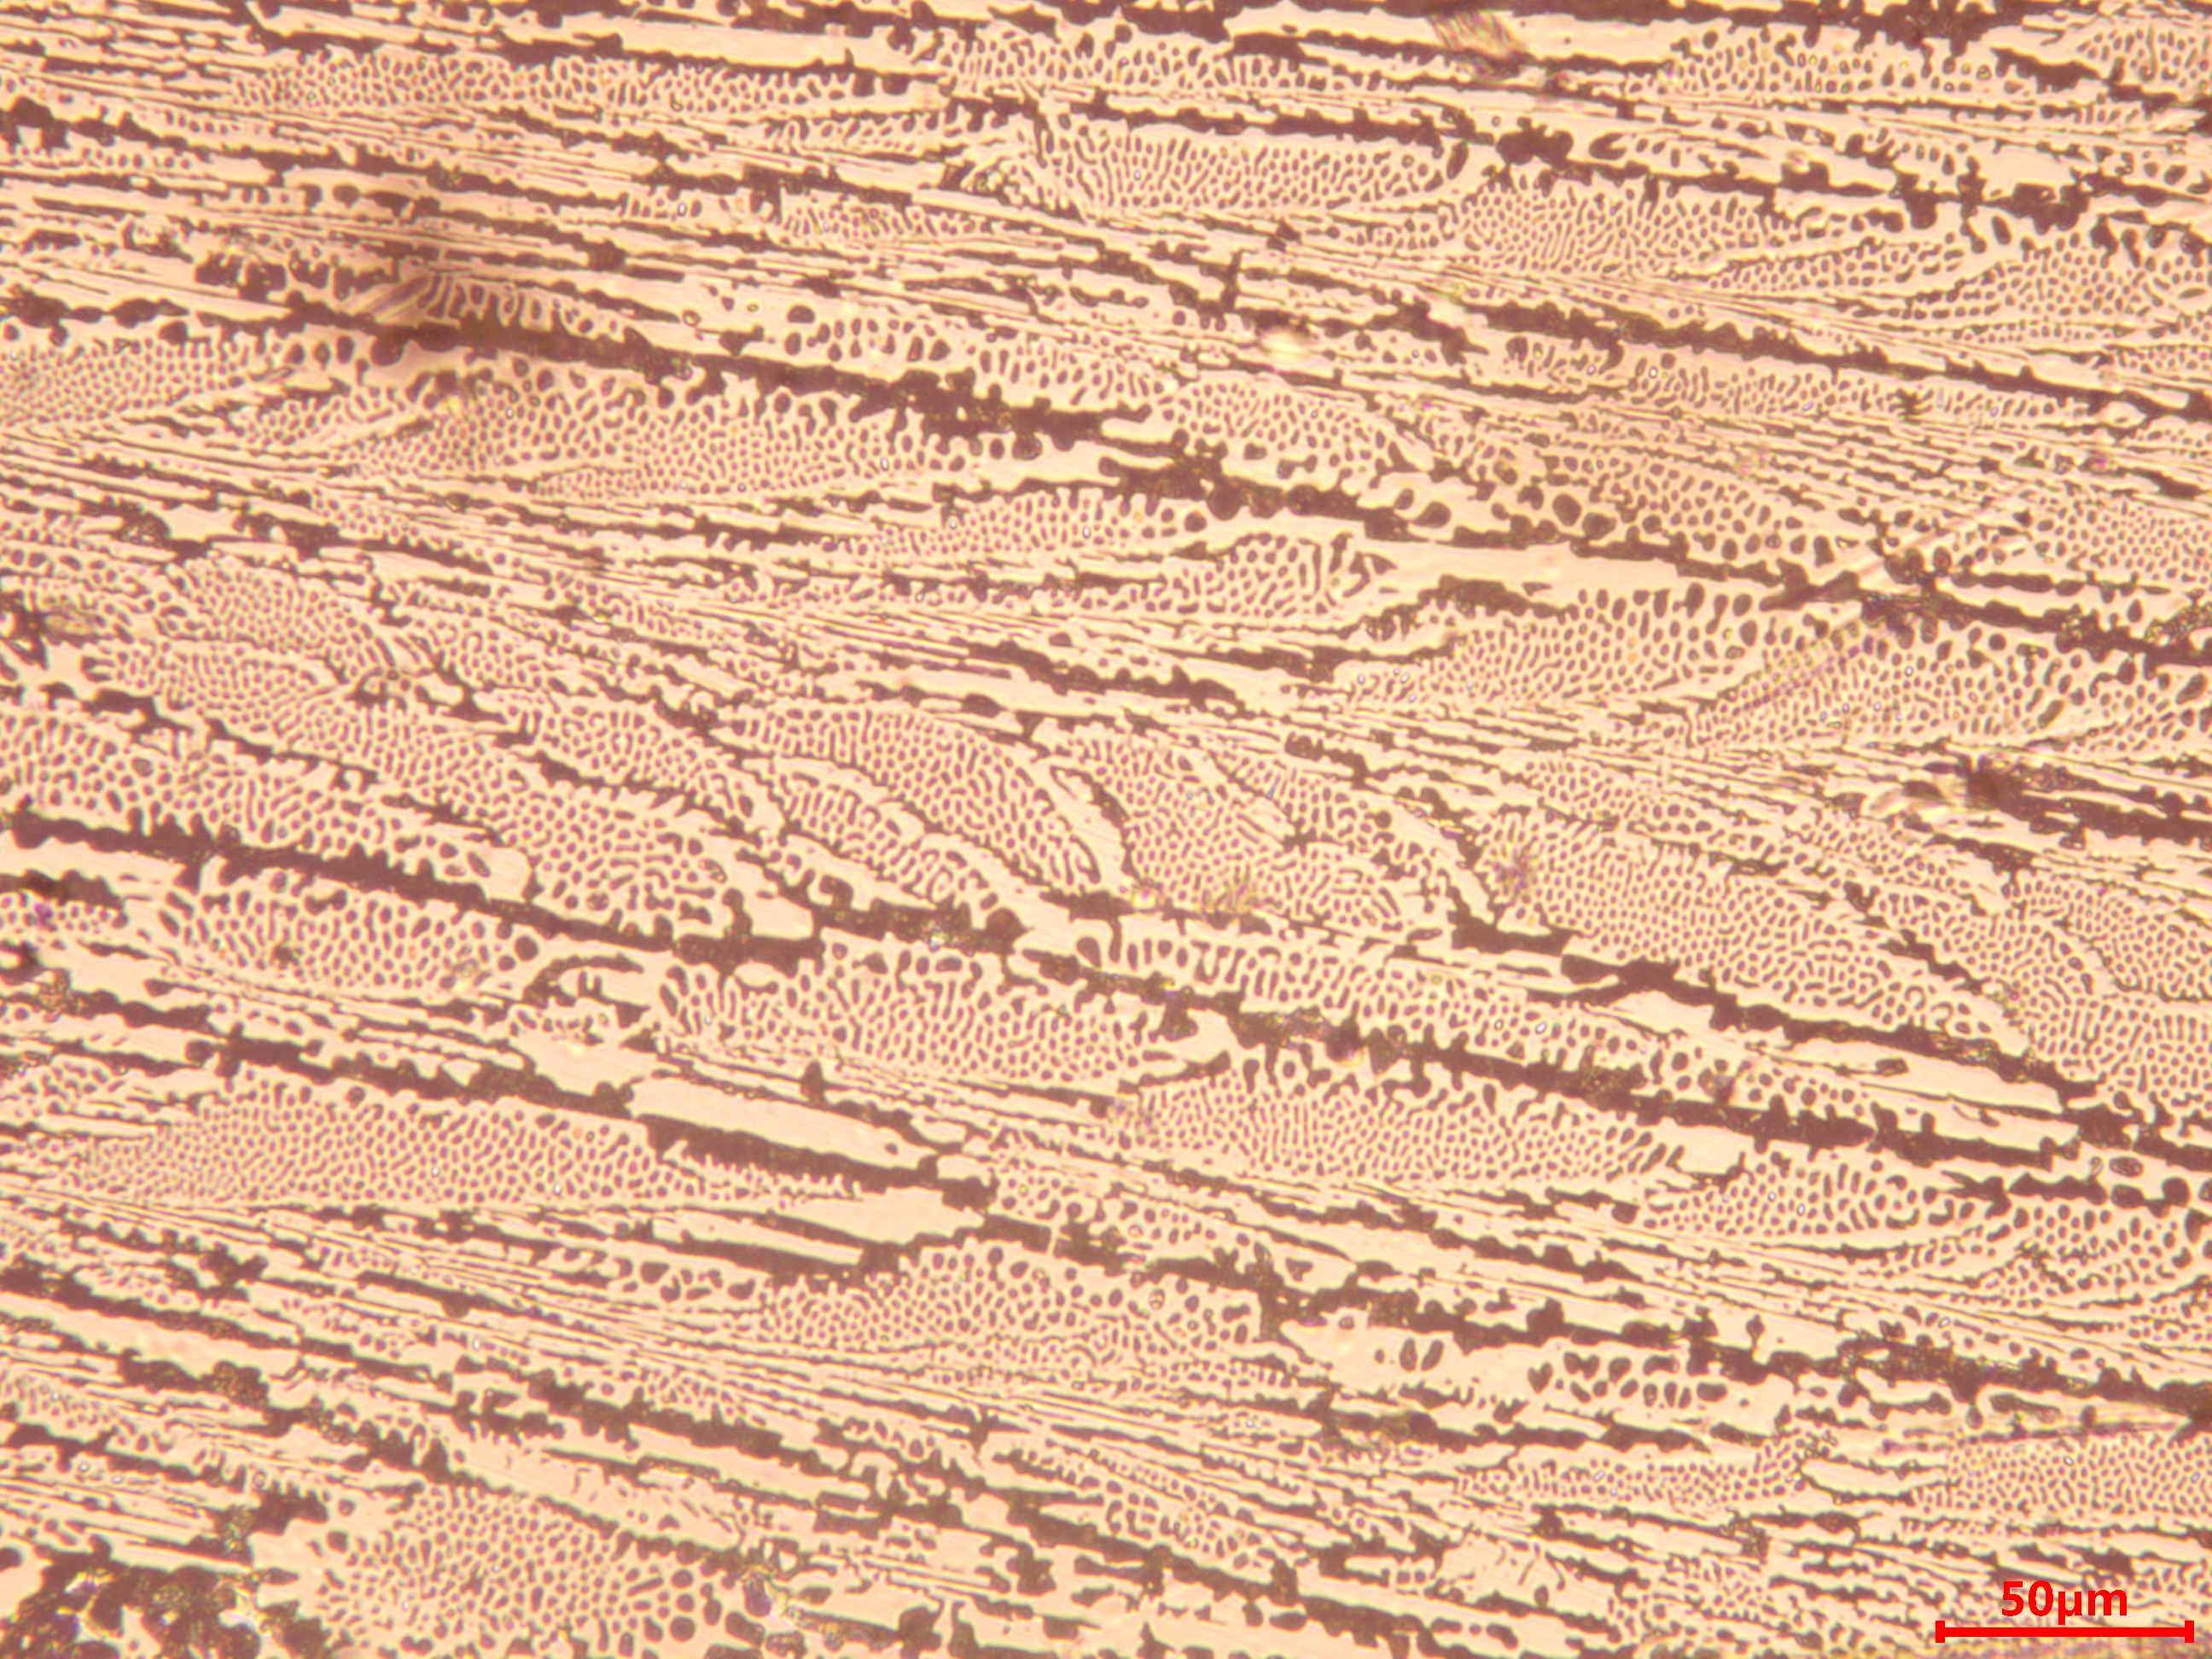
\includegraphics[height=24mm]{img/A1/09_200x.jpg}}\hspace{20pt}
        \subfloat[$500\times{}$]{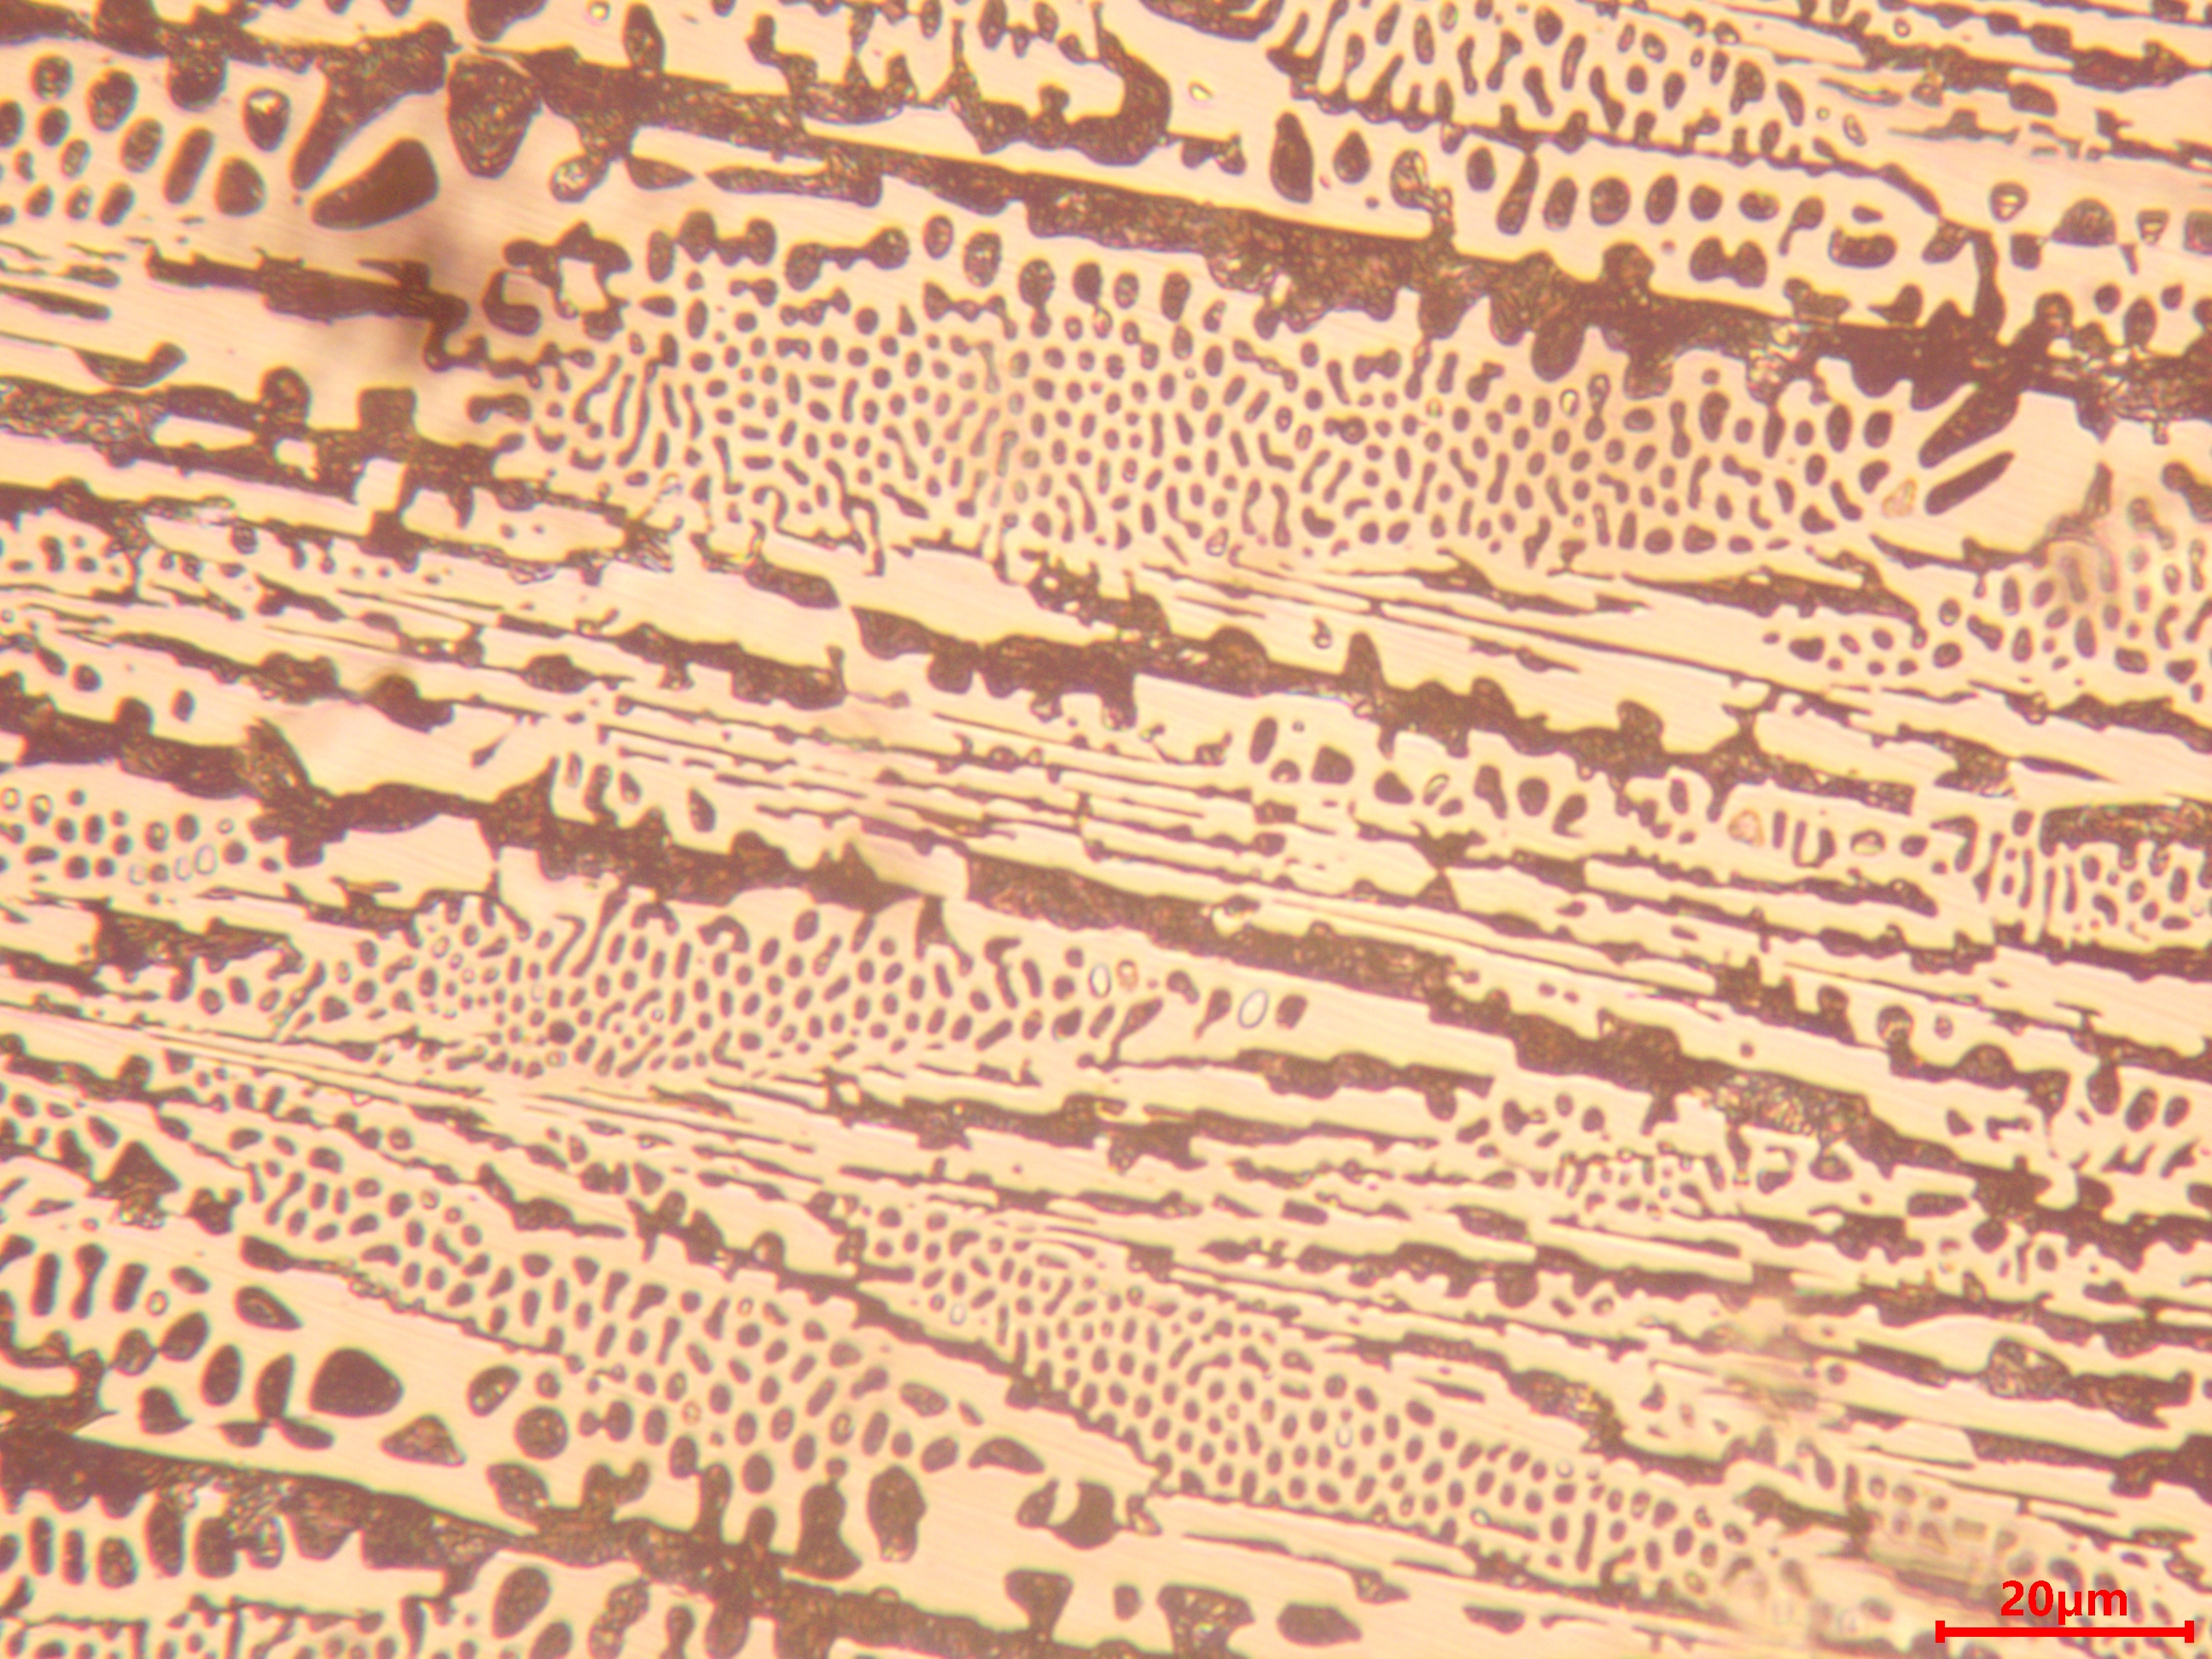
\includegraphics[height=24mm]{img/A1/09_500x.jpg}}\hspace{20pt}
        \subfloat[手绘图]{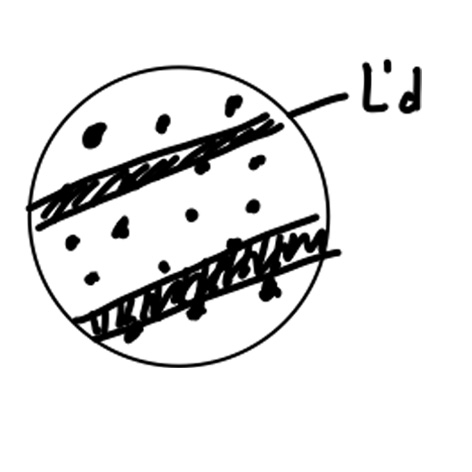
\includegraphics[height=24mm]{img/A1/n6.jpg}}
        \caption{共晶白口铸铁显微组织\label{fig:n6}}
    \end{figure}

    \subsubsection{过共晶白口铸铁}
    过共晶白口铸铁含碳量为$4.3\%\sim 6.69\%$,室温下的显微组织由一次渗碳体 $\text{Fe}_3\text{C}_\text{I}$ 和低温莱氏体($\text{L}_\text{d}^{'}$)构成,其中的一次渗碳体呈白亮色板条状分布在低温莱氏体中,如\fgref{fig:n7} 所示。
    \begin{figure}[!ht]
        \subfloat[$200\times{}$]{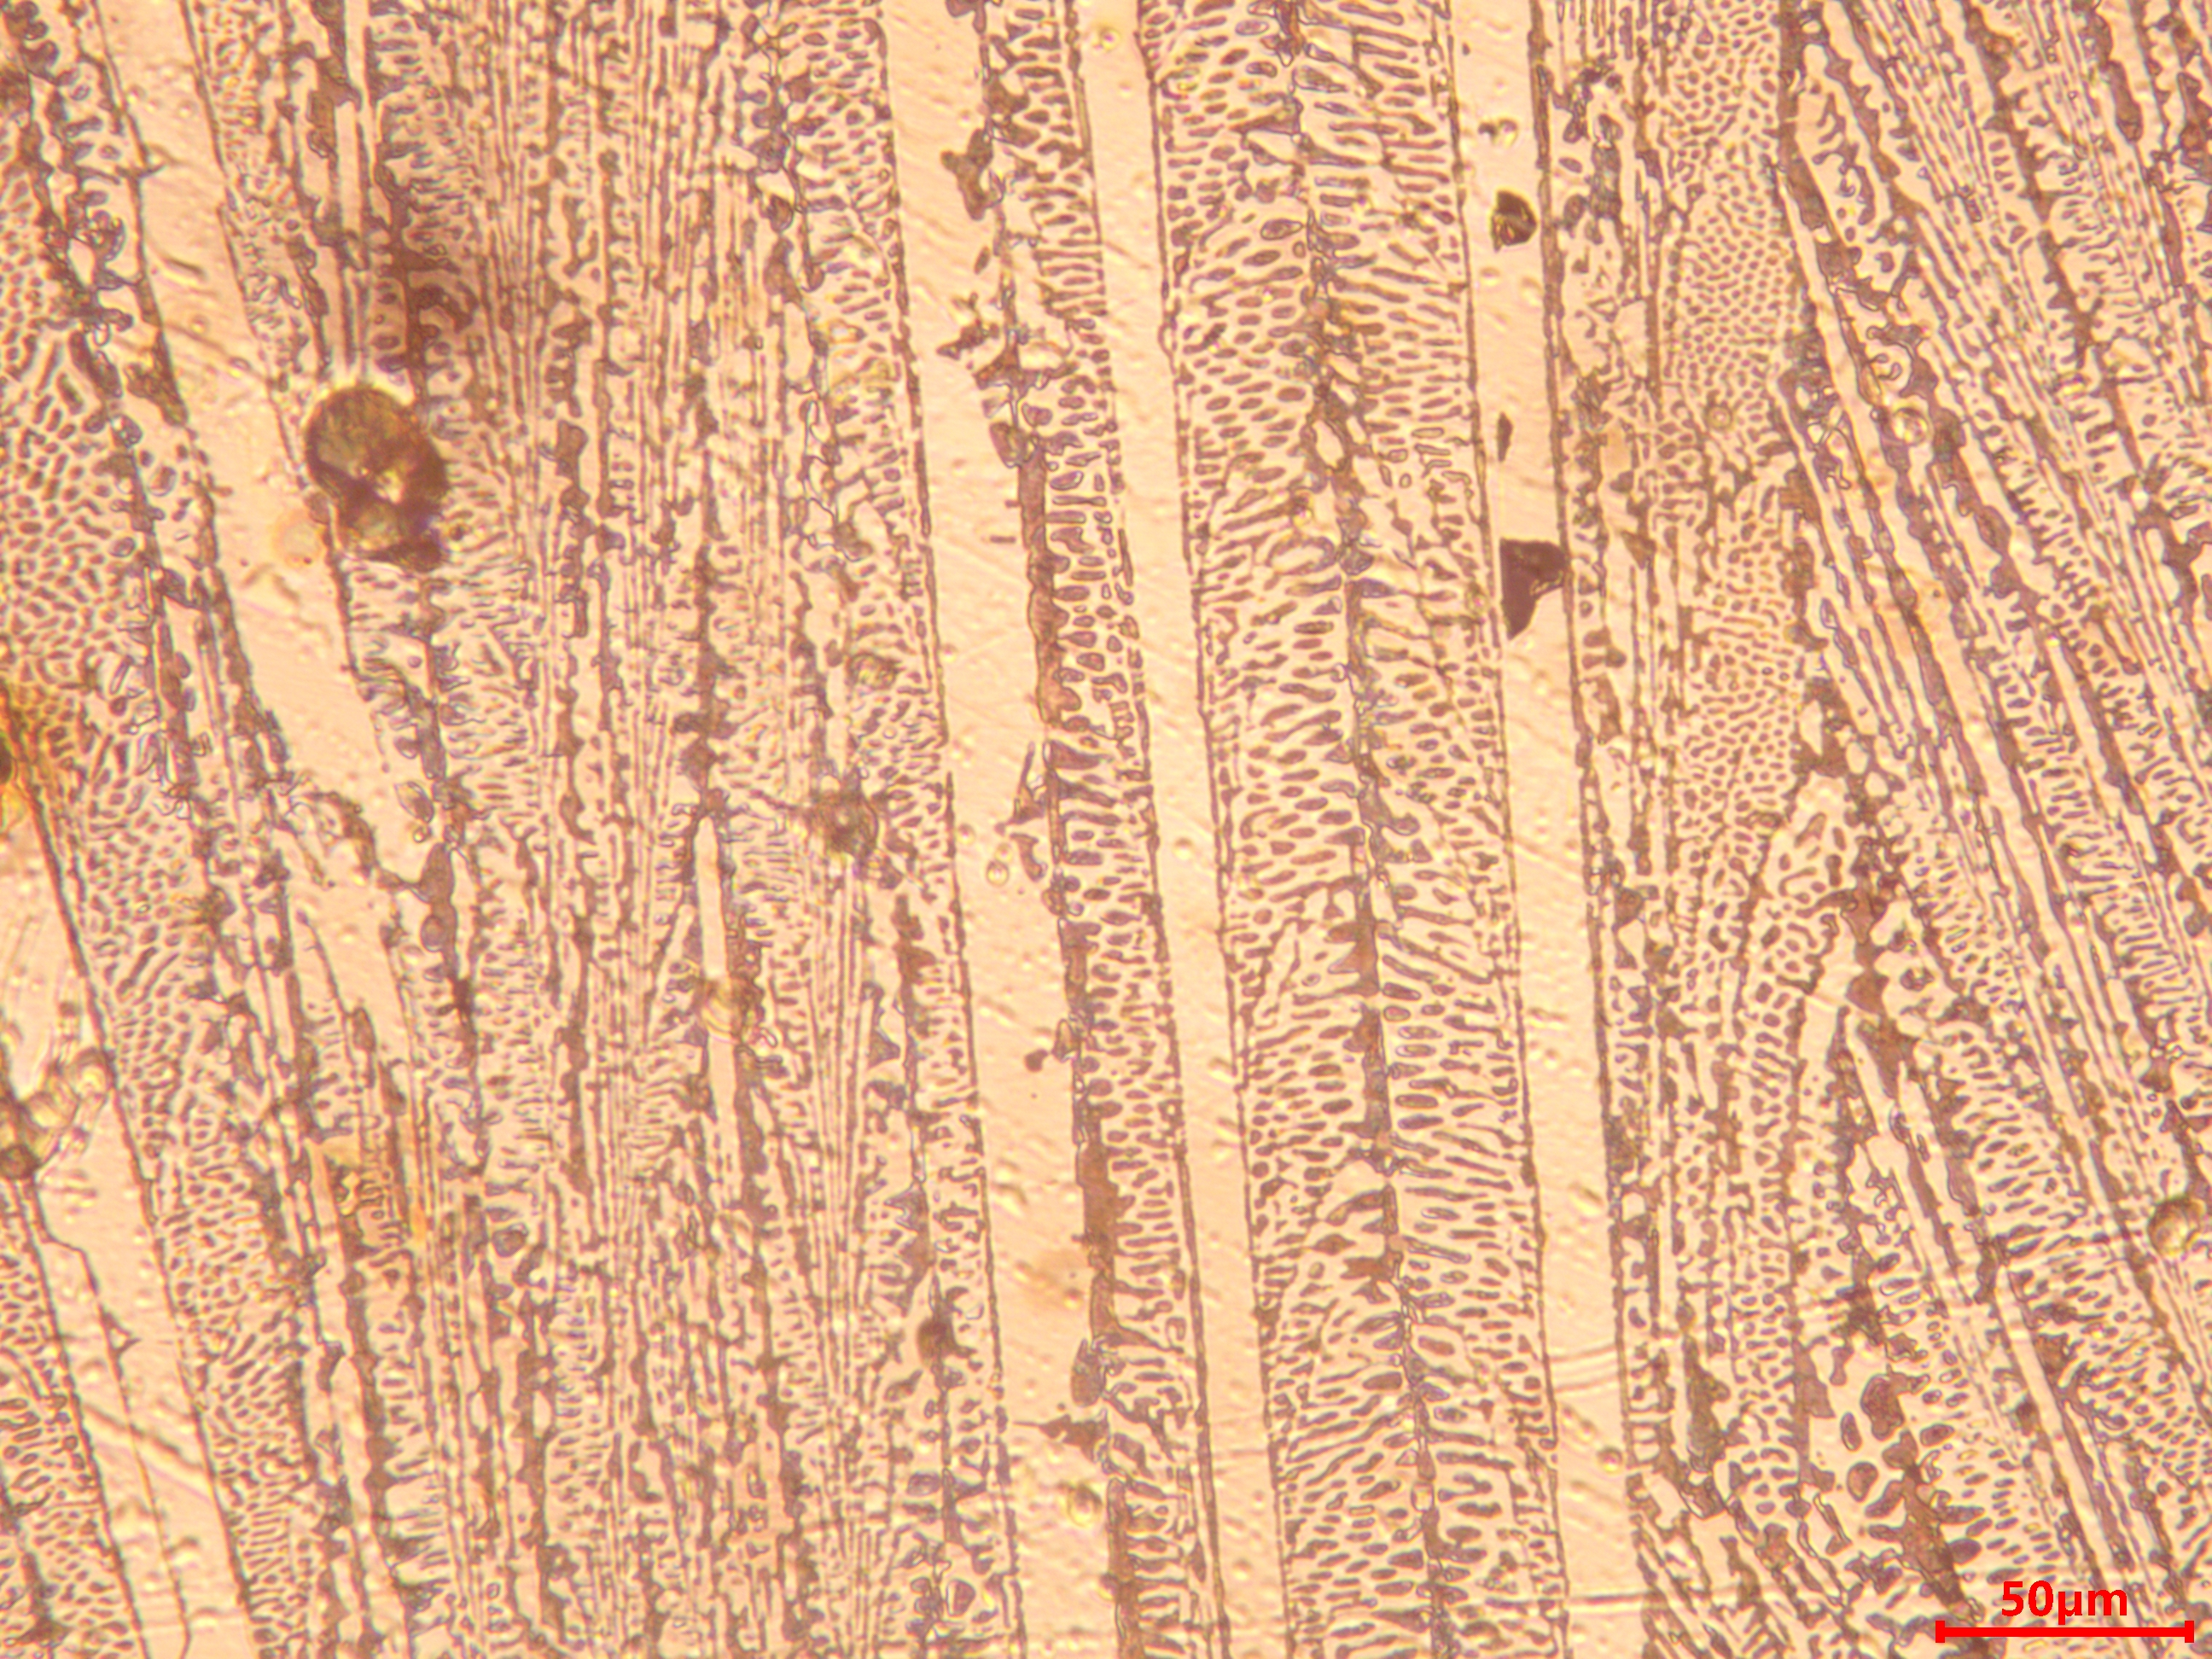
\includegraphics[height=24mm]{img/A1/10_200x.jpg}}\hspace{20pt}
        \subfloat[$500\times{}$]{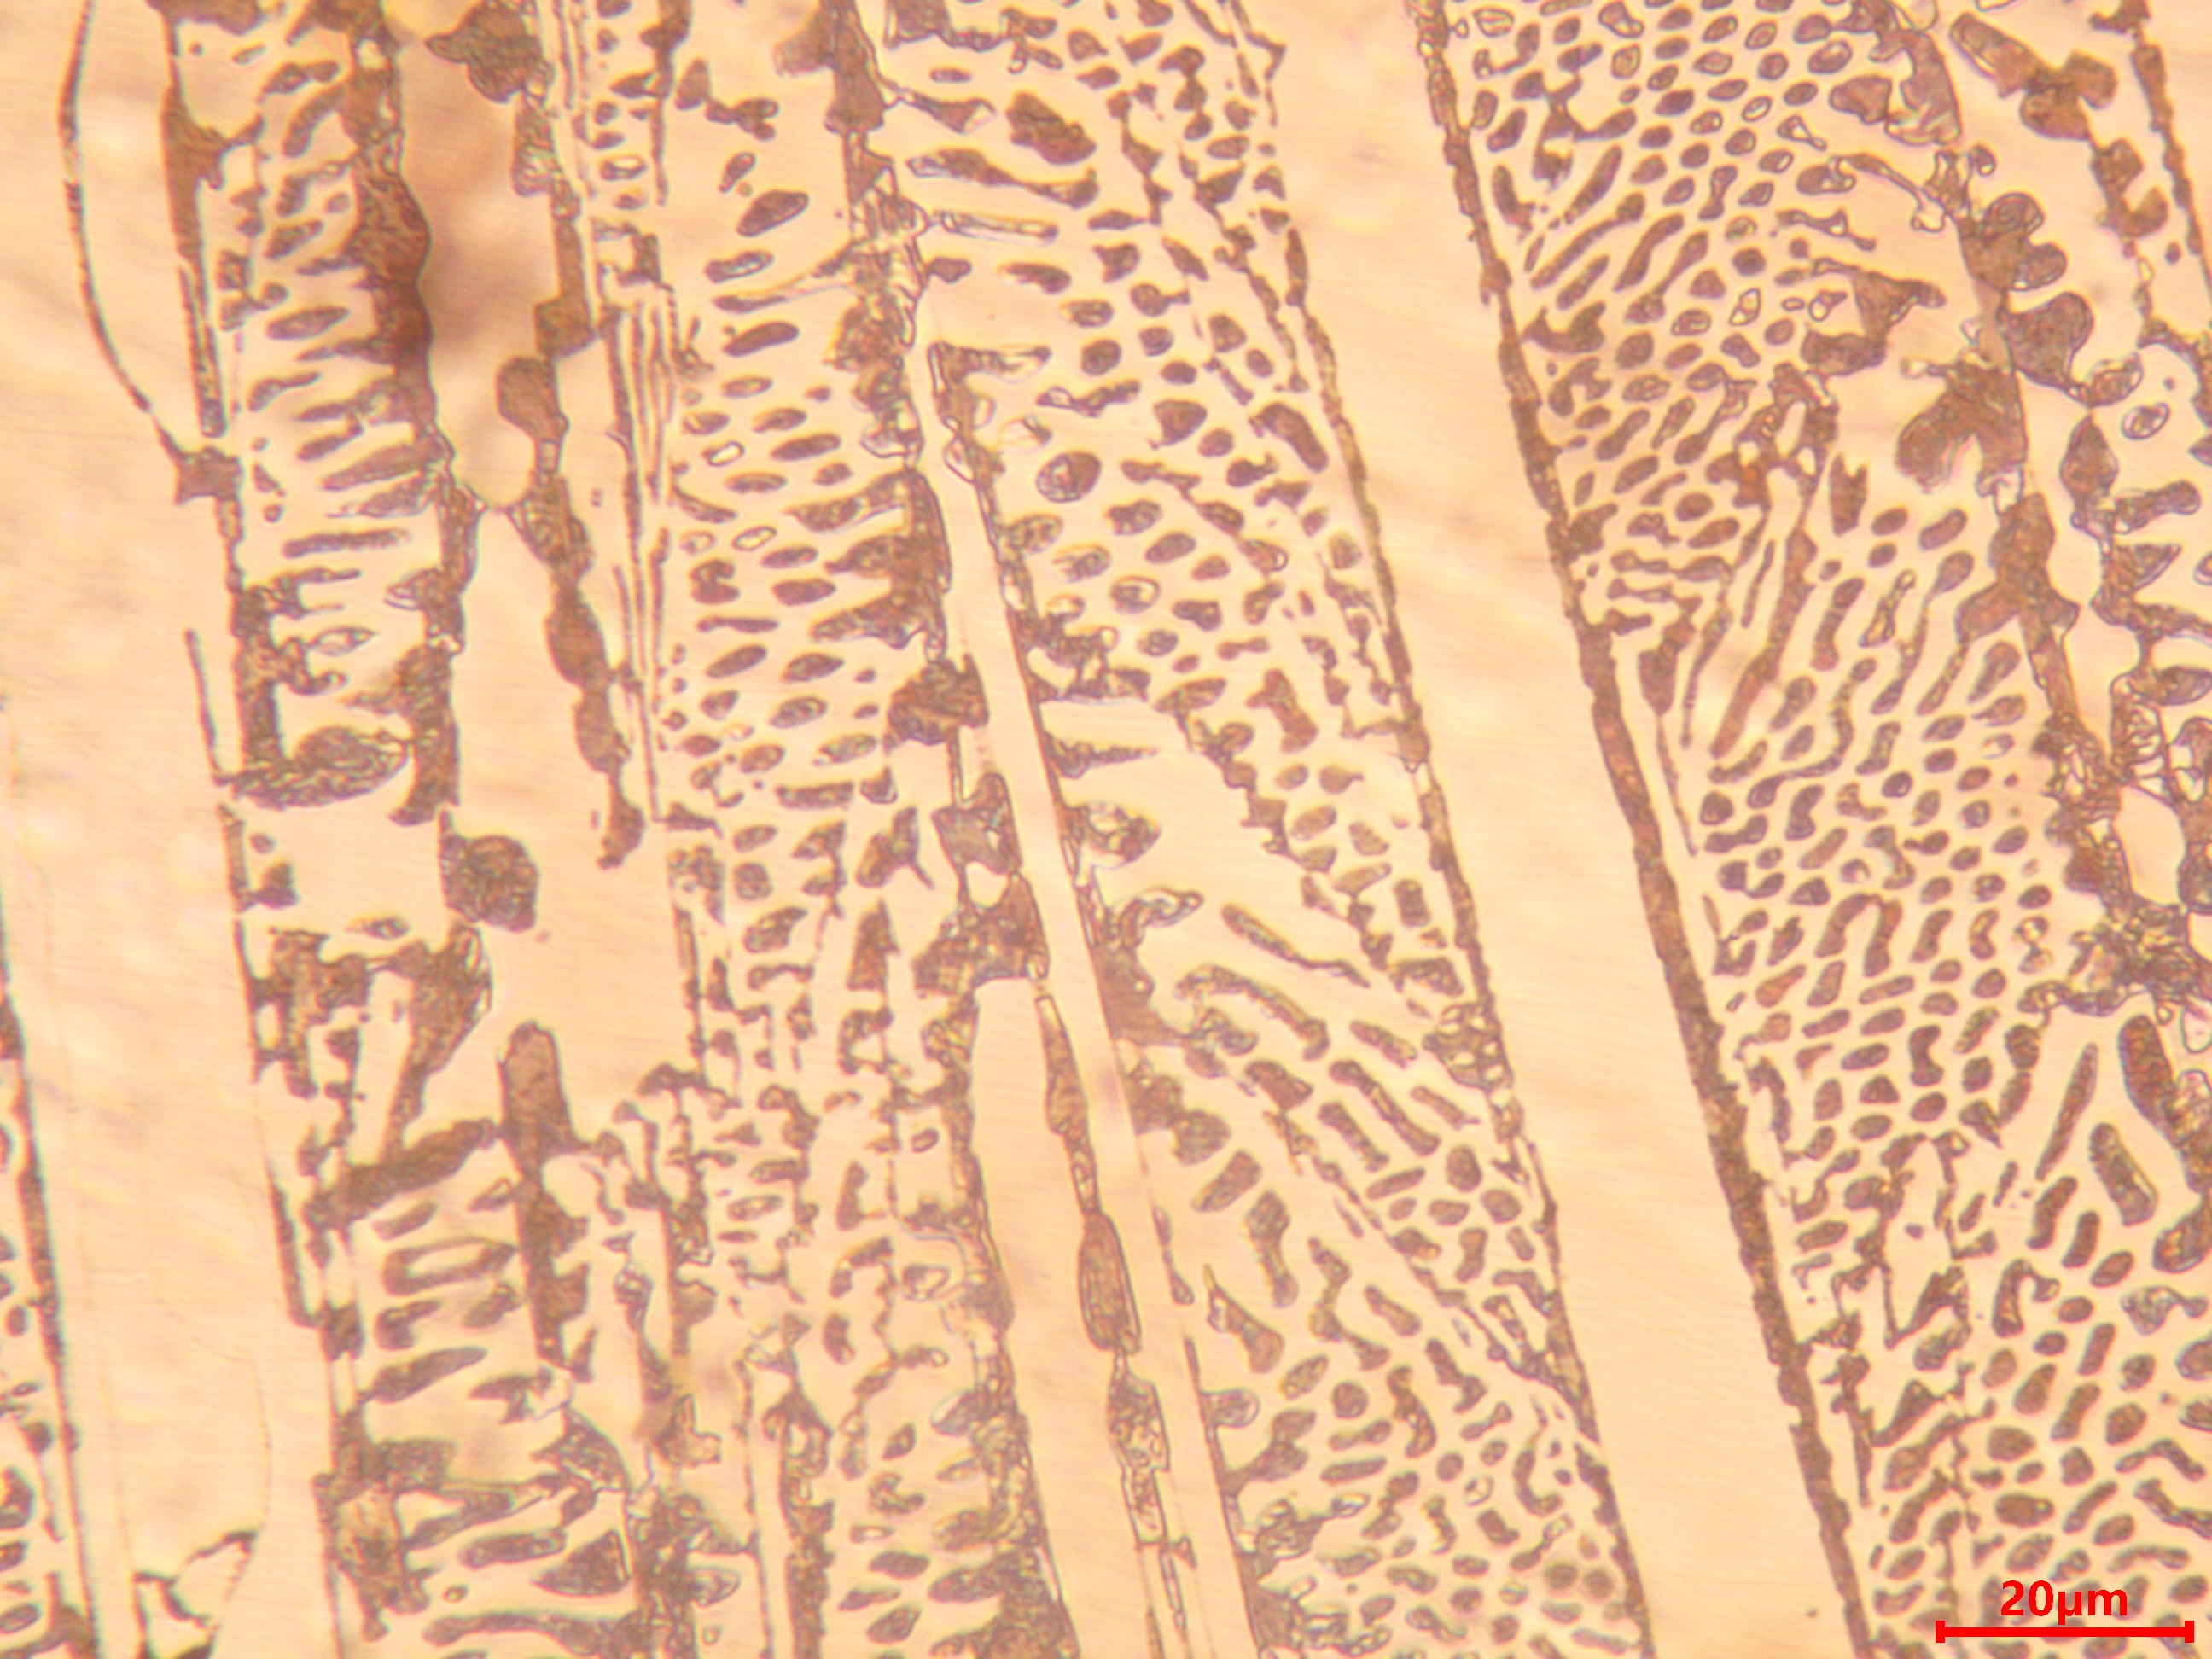
\includegraphics[height=24mm]{img/A1/10_500x.jpg}}\hspace{20pt}
        \subfloat[手绘图]{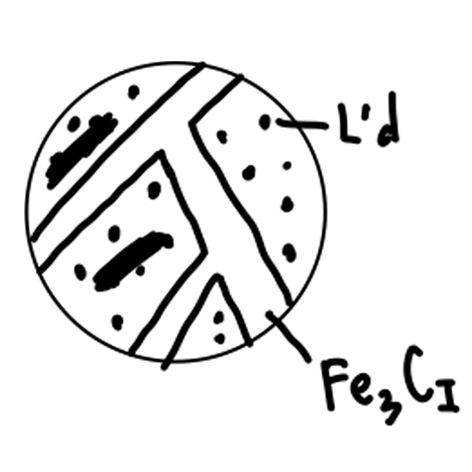
\includegraphics[height=24mm]{img/A1/n7.jpg}}
        \caption{过共晶白口铸铁显微组织\label{fig:n7}}
    \end{figure}
    \newpage
    \subsection{铁碳合金室温下的非平衡组织}
    钢经过热处理后所得到的组织与室温下的平衡组织有很大区别,称为铁碳合金的非平衡组织。\par

    \subsubsection{45 钢 \SI{860}{\degreeCelsius} 水淬 $+$ 中温回火\label{ss2:45sczw}}
    从\fgref{fig:n8} 可见,图中主要的组织是回火屈氏体。钢经淬火后,在 \SI{400}{\degreeCelsius} 左右回火时所形成的极易腐蚀的组织叫做屈氏体。这时,马氏体针状形态消失, 但仍隐约可见, 回火时析出的碳化物细小,在光学显微镜下难以分辩清楚。
    \begin{figure}[!ht]
        \subfloat[$200\times{}$]{\includegraphics[height=24mm]{img/A1/21_200x.jpg}}\hspace{20pt}
        \subfloat[$500\times{}$]{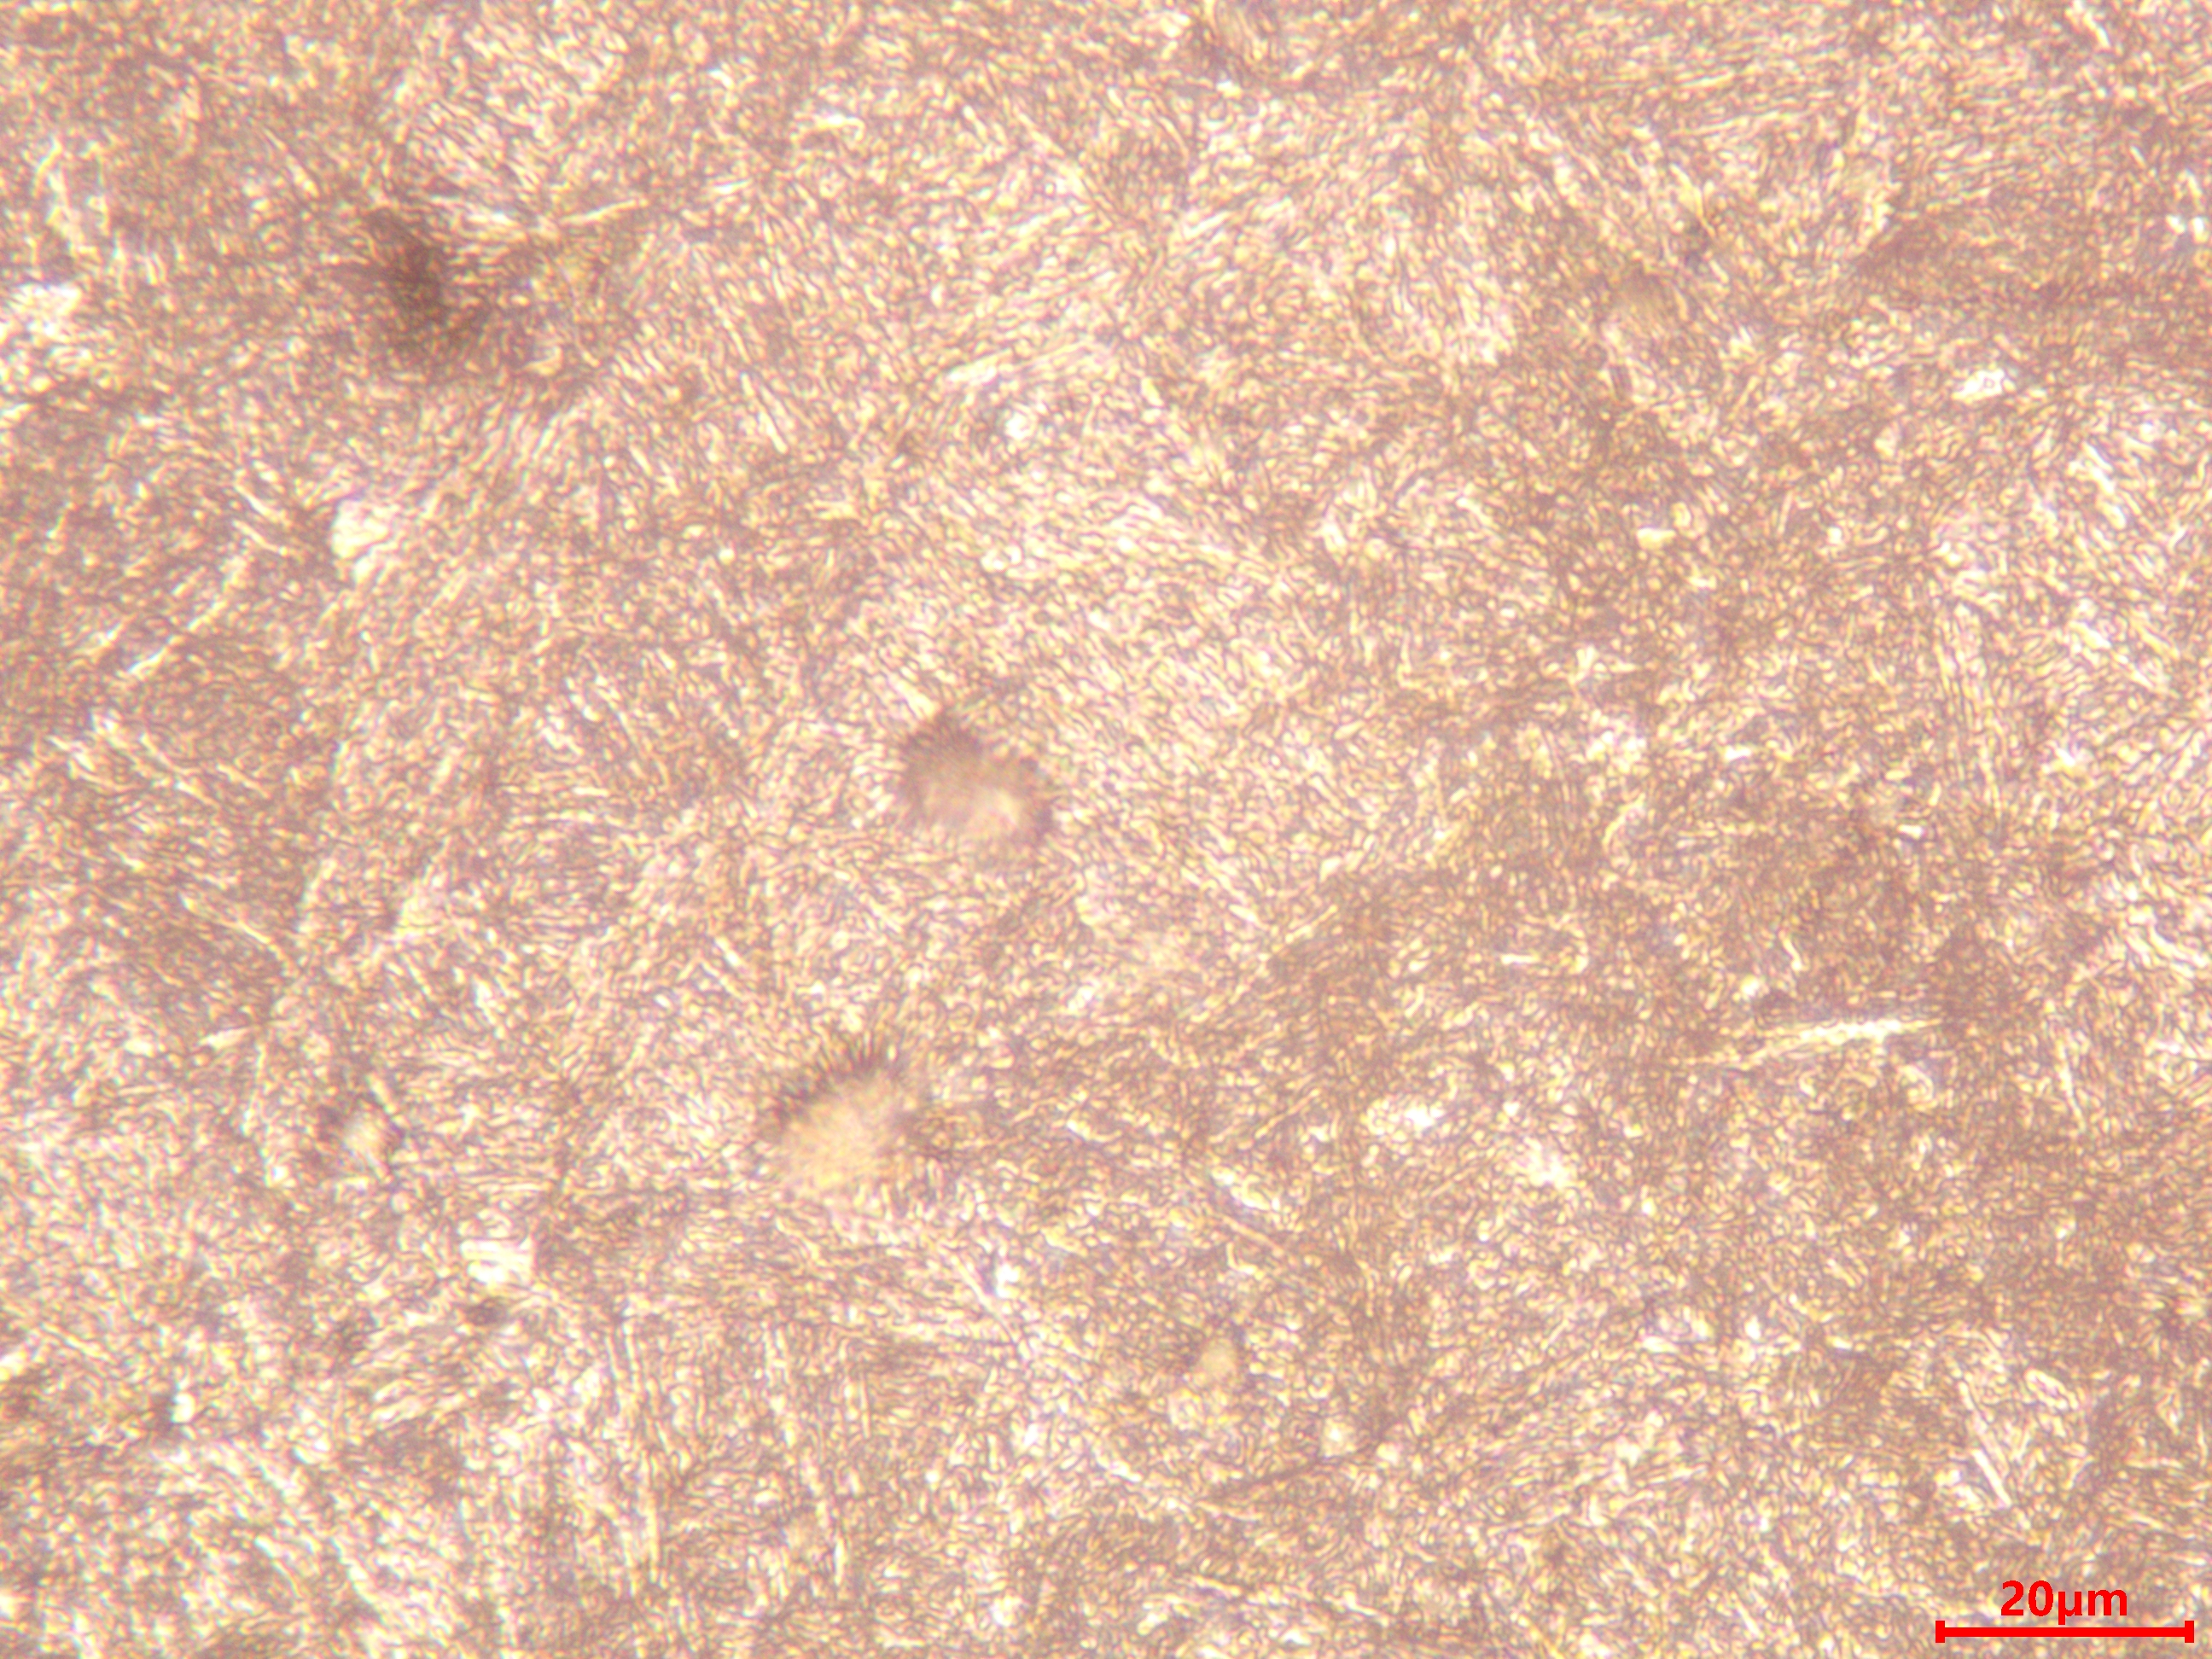
\includegraphics[height=24mm]{img/A1/21_500x.jpg}}
        \caption{45 钢 \SI{860}{\degreeCelsius} 水淬 $+$ 中温回火显微组织\label{fig:n8}}
    \end{figure}

    \subsubsection{45 钢 \SI{860}{\degreeCelsius} 水淬 $+$ 高温回火\label{ss2:45scgw}}
    从\fgref{fig:n9} 可见,图中主要的组织是回火索氏体。淬火钢在 \SI{600}{\degreeCelsius} 以上回火时,所形成的组织叫索氏体,这种组织特点是索氏体基体上中弥散分布着细小的球(颗粒)状渗碳体,在光学显微镜下能分辨清楚。索氏体硬度一般在 280HV 左右。\par
    对比 \Nameref{ss2:45sczw} 和 \Nameref{ss2:45scgw} ,可以知道回火温度越高,颗粒状的渗碳体越来越明显,而马氏体的形态逐渐消失.回火温度不同导致了不同的最终形态。
    \begin{figure}[!ht]
        \subfloat[$200\times{}$]{\includegraphics[height=24mm]{img/A1/22_200x.jpg}}\hspace{20pt}
        \subfloat[$500\times{}$]{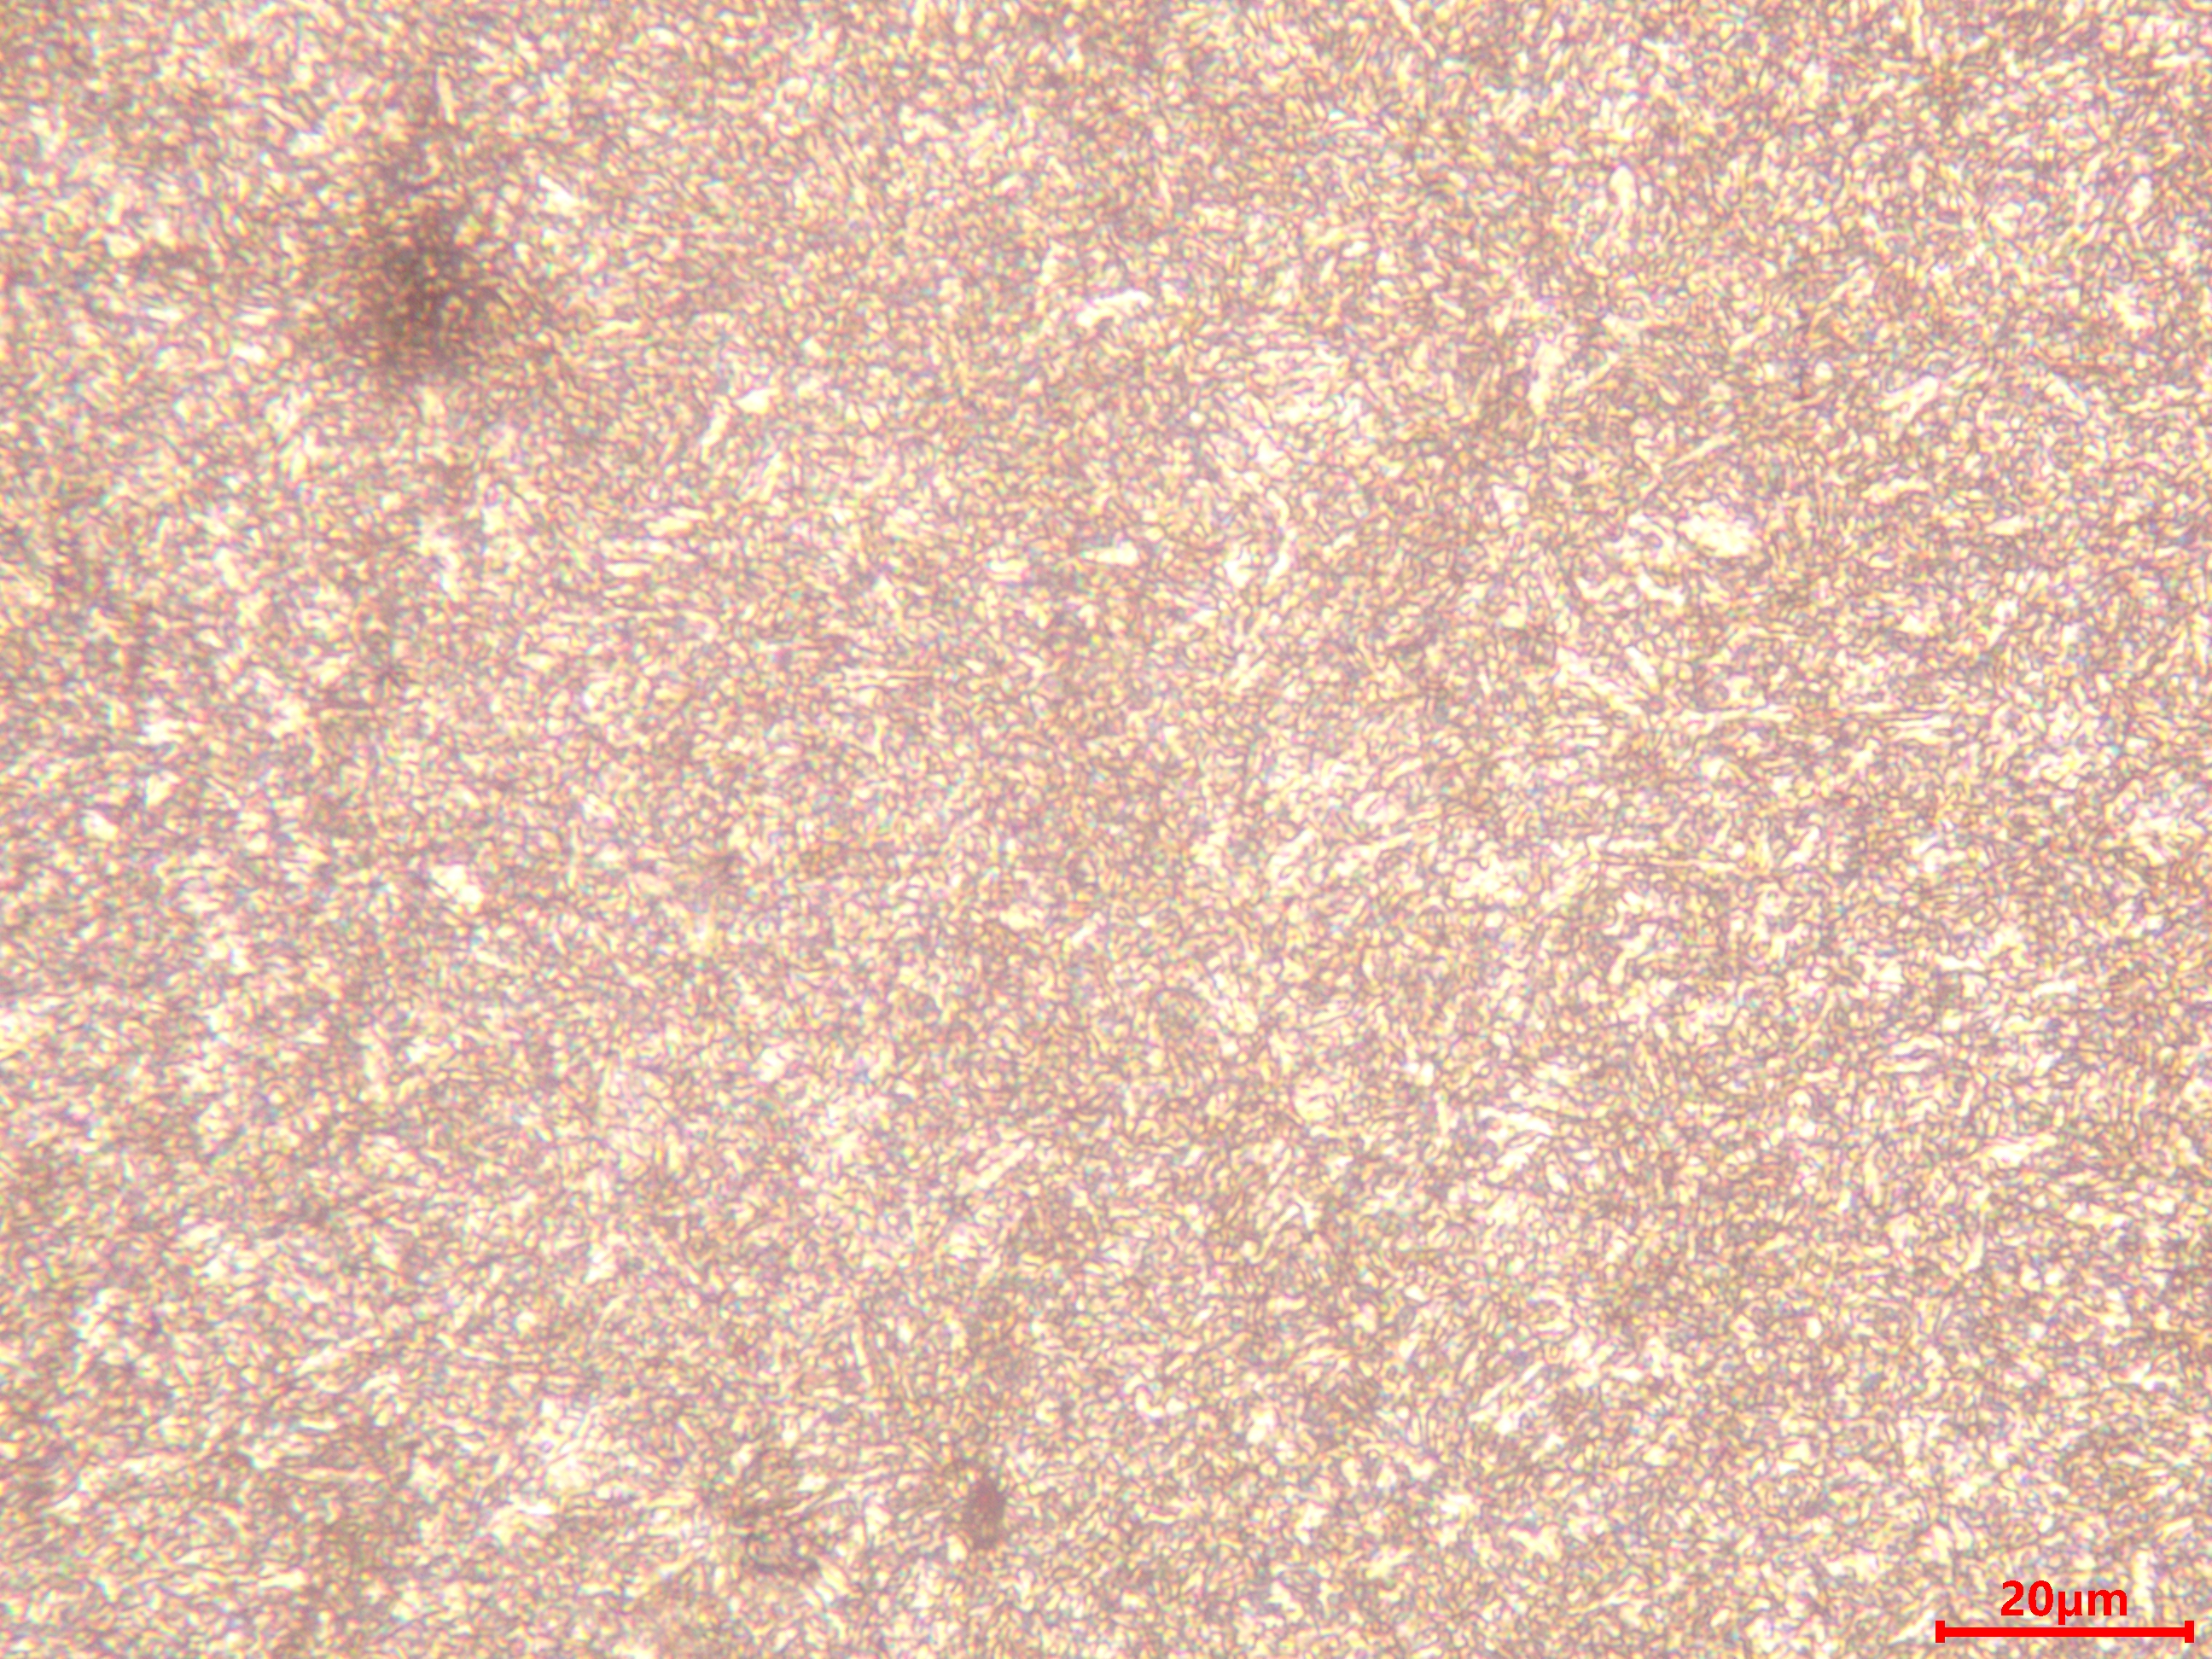
\includegraphics[height=24mm]{img/A1/22_500x.jpg}}
        \caption{45 钢 \SI{860}{\degreeCelsius} 水淬 $+$ 高温回火显微组织\label{fig:n9}}
    \end{figure}

    \subsubsection{45 钢 \SI{780}{\degreeCelsius} 水淬\label{ss2:45_780}}
    从\fgref{fig:n10} 中可见,图中主要的组织是马氏体和白色的铁素体。
    \begin{figure}[!ht]
        \subfloat[$200\times{}$]{\includegraphics[height=24mm]{img/A1/23_200x.jpg}}\hspace{20pt}
        \subfloat[$500\times{}$]{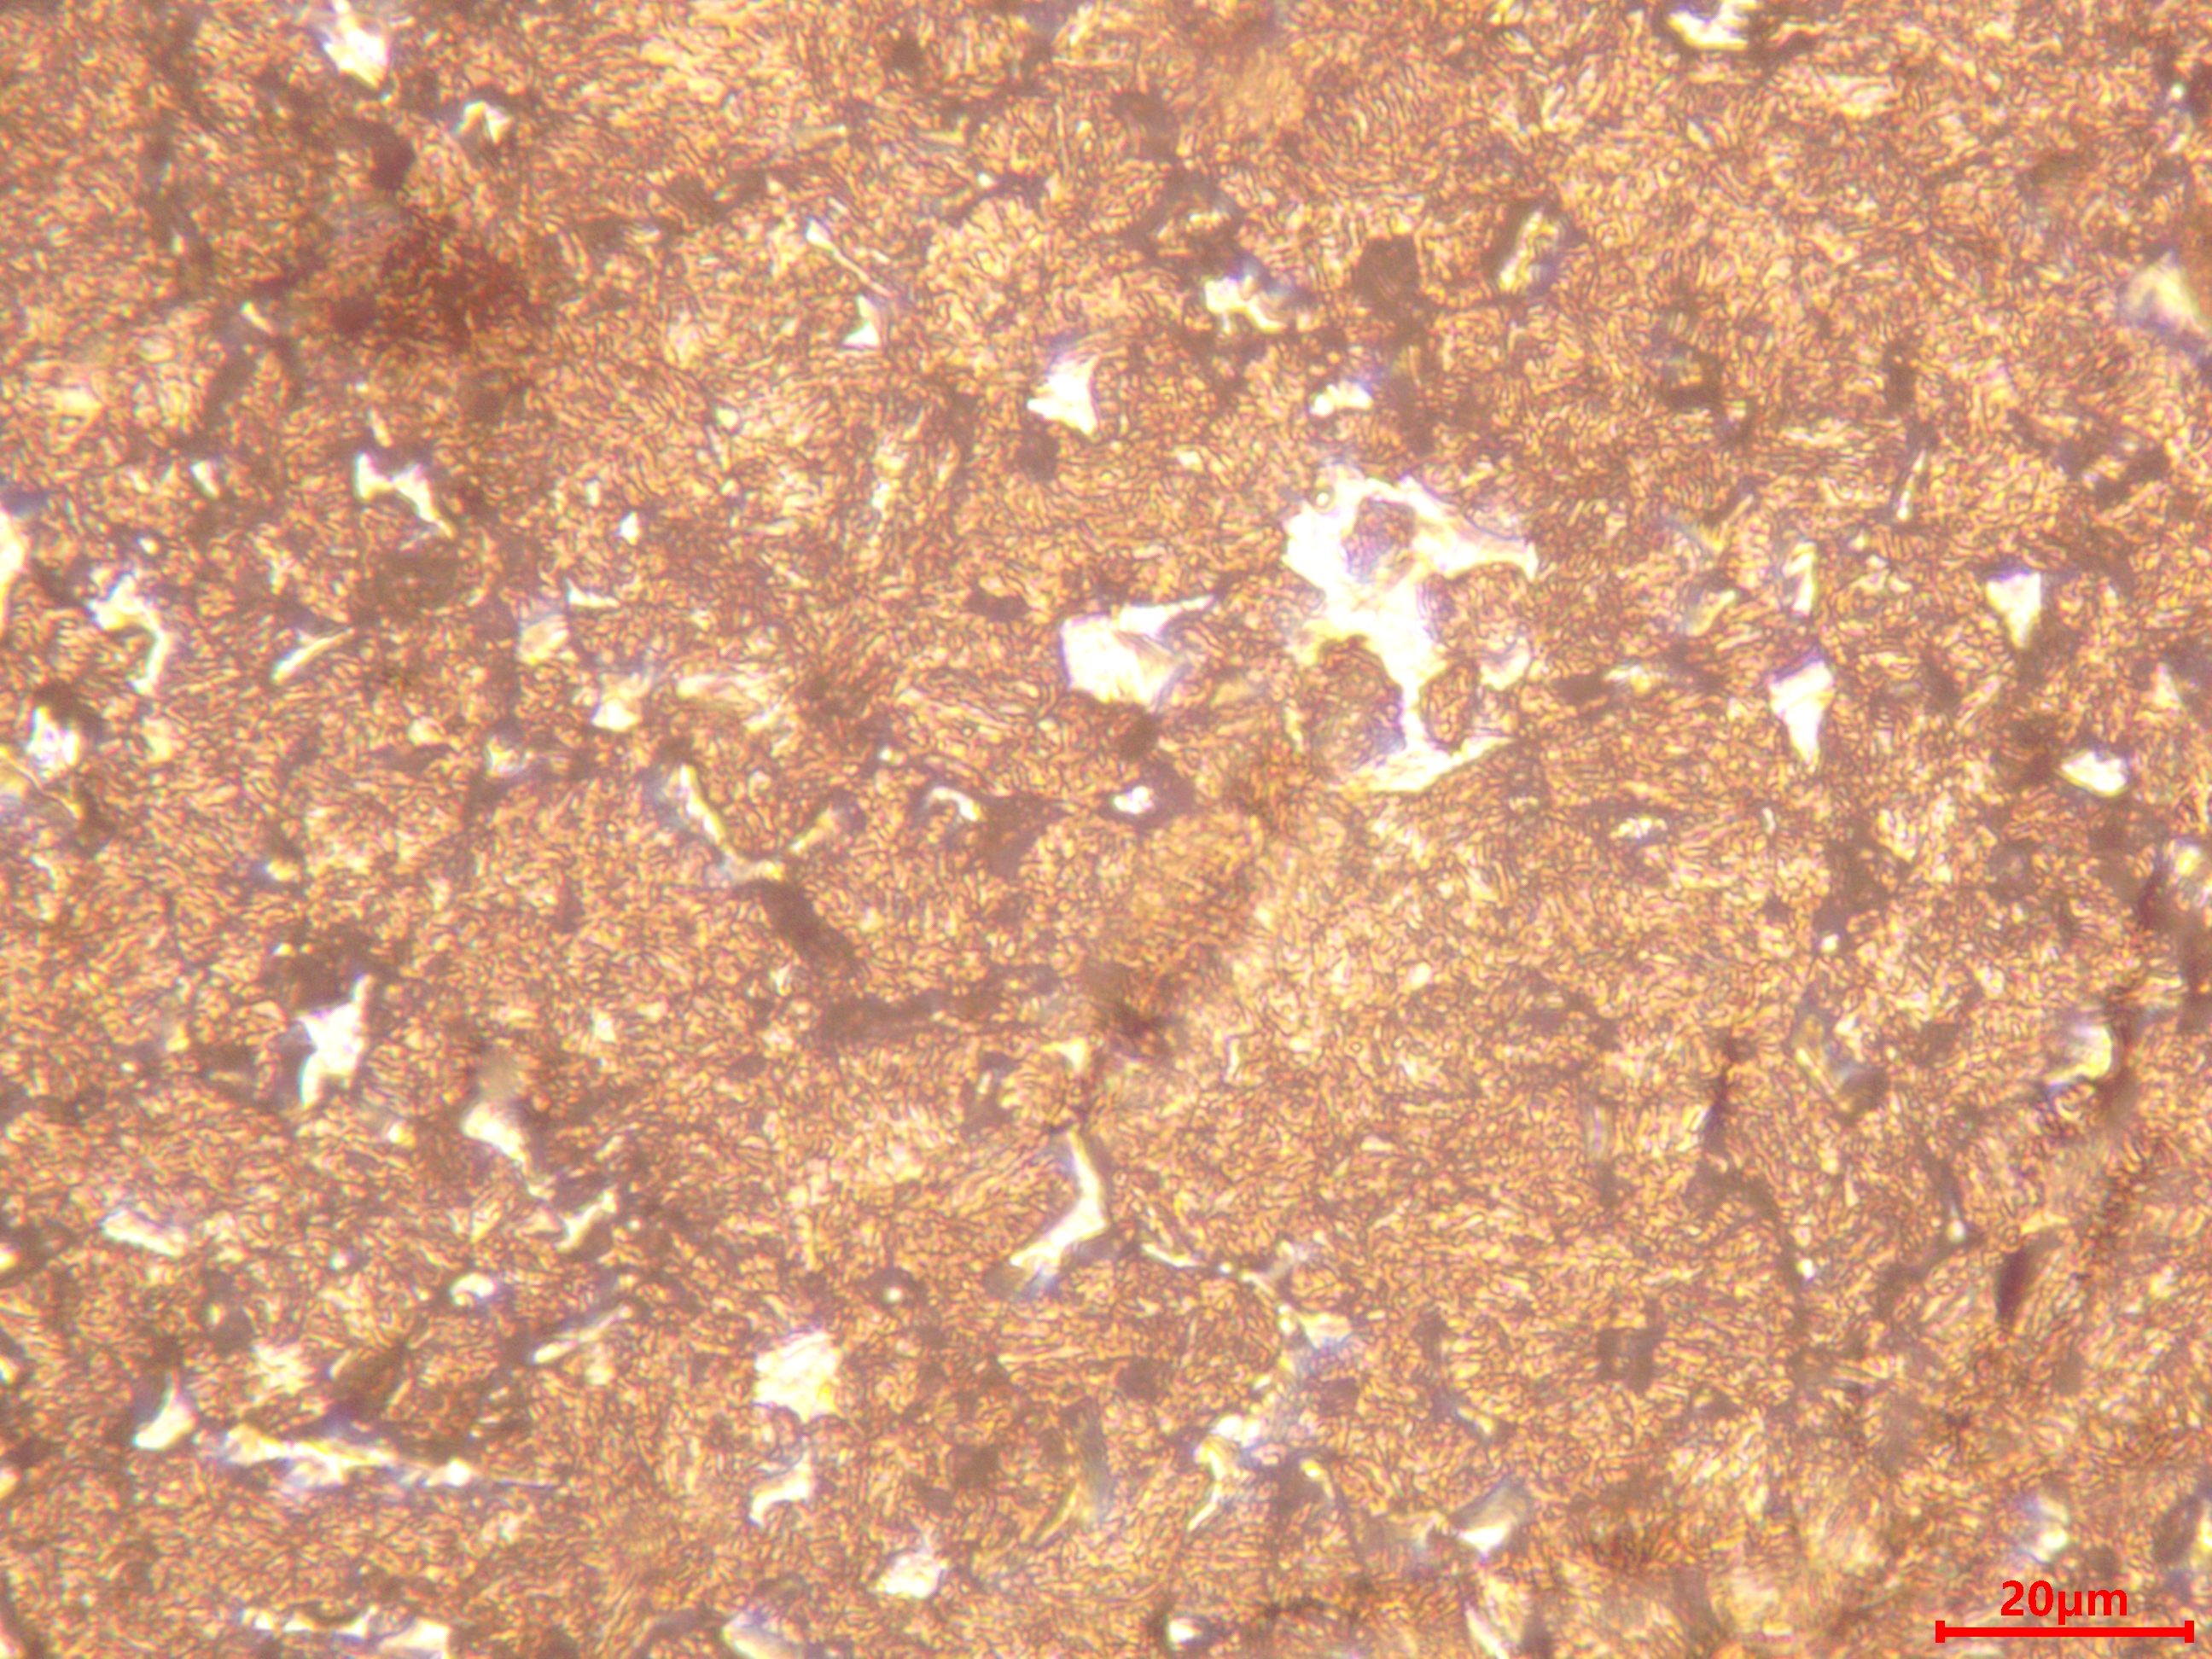
\includegraphics[height=24mm]{img/A1/23_500x.jpg}}
        \caption{45 钢 \SI{780}{\degreeCelsius} 水淬显微组织\label{fig:n10}}
    \end{figure}

    \subsubsection{45 钢 \SI{1100}{\degreeCelsius} 水淬\label{ss2:45_1100}}
    从\fgref{fig:n11} 中可见,图中主要的组织是针线状的马氏体与白色的铁素体。马氏体是碳在$\alpha\text{-Fe}$ 晶格中的过饱和固溶体, 马氏体组织是奥氏体(溶有充足的碳原子) 过冷到低温区(如 \SI{240}{\degreeCelsius} 以下) 在连续冷却过程中形成。
	对比 \Nameref{ss2:45_780} 和 \Nameref{ss2:45_1100} 可知,由于两个样品的水淬温度不同,最后形成的组织成分与组织形态均不同。\Nameref{ss2:45_1100} 的样品在水淬时的温度是 \SI{1100}{\degreeCelsius},对应奥氏体单相区,故水冷以后为单相马氏体,而且由于过热,马氏体的形态明显。而 \Nameref{ss2:45_780} 的样品在 \SI{780}{\degreeCelsius} 水淬,对应奥氏体与铁素体的两相区,故最终水冷后为马氏体与铁素体。

    \begin{figure}[!ht]
        \subfloat[$200\times{}$]{\includegraphics[height=24mm]{img/A1/24_200x.jpg}}\hspace{20pt}
        \subfloat[$500\times{}$]{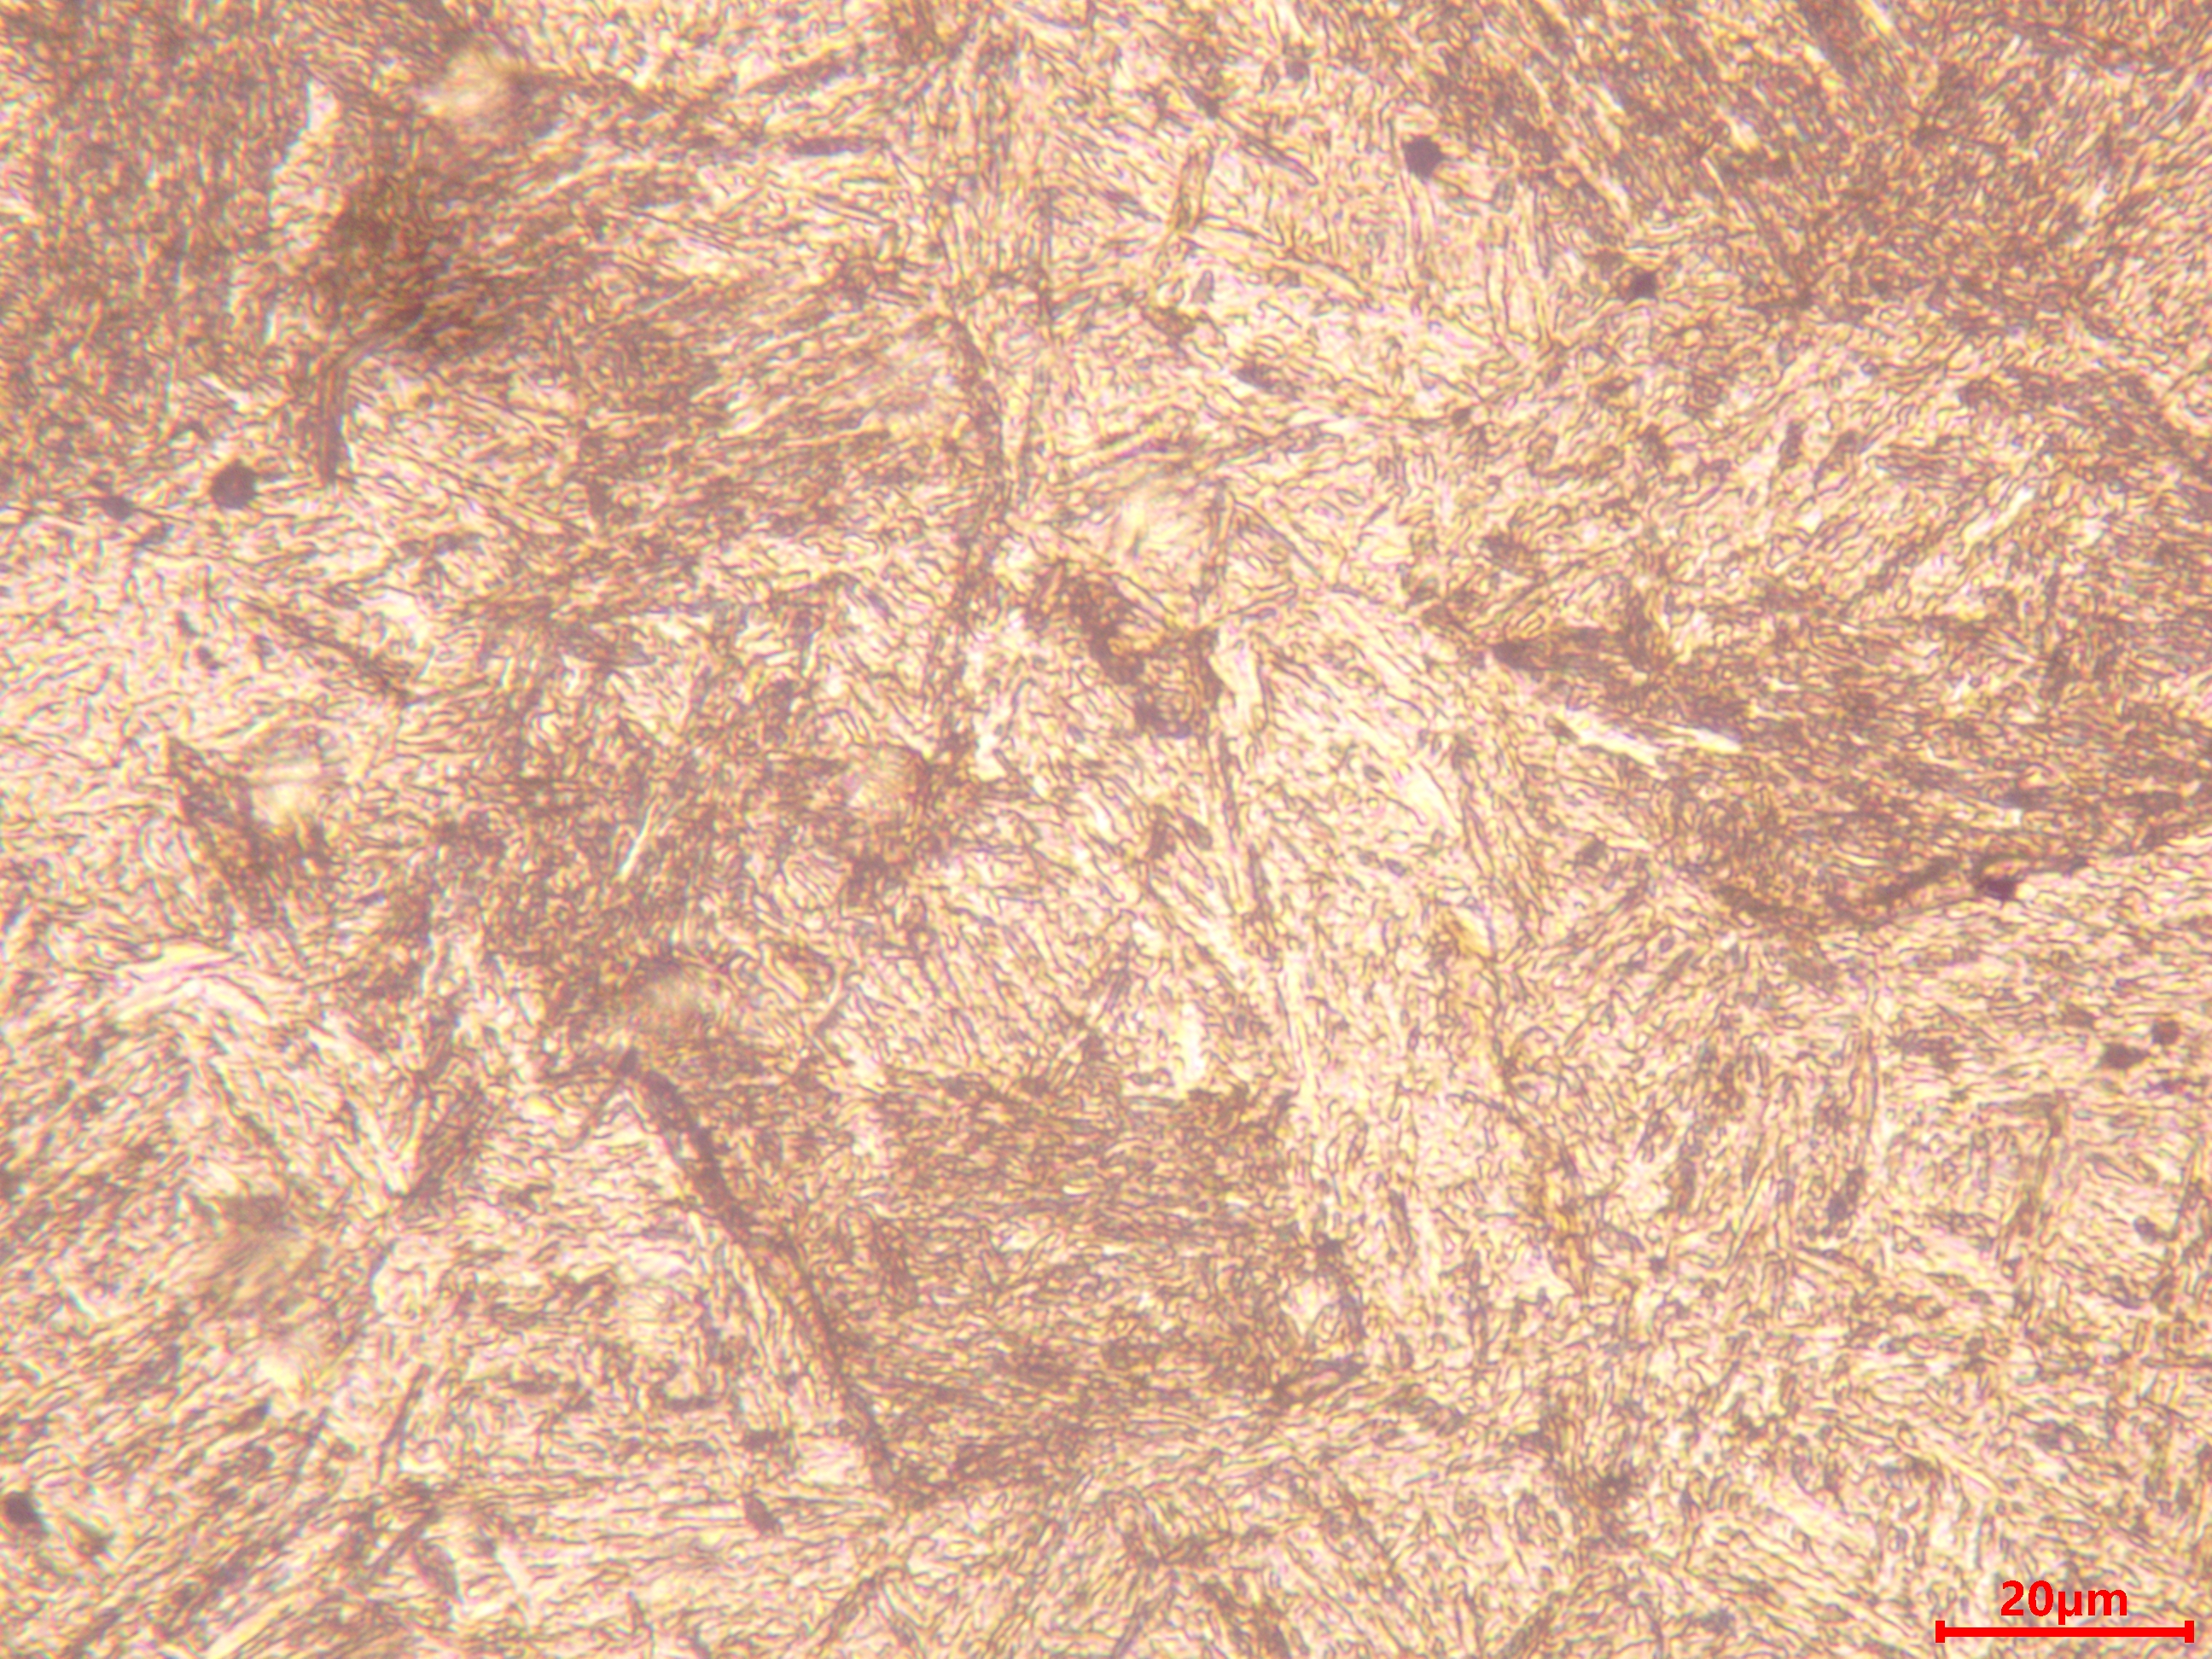
\includegraphics[height=24mm]{img/A1/24_500x.jpg}}
        \caption{45 钢 \SI{1100}{\degreeCelsius} 水淬显微组织\label{fig:n11}}
    \end{figure}

    \subsubsection{T12 钢球化退火}
    球化退火是使钢中碳化物球化而进行的退火,得到在铁素体基体上均匀分布的球状或颗粒状碳化物的组织。球化退火主要用于共析钢和过共析钢,以获得类似粒状珠光体的球化组织(因不一定是共析成分,故称为球化组织)。从\fgref{fig:n12} 中可以看到许多类似圆圈状的渗碳体球。
    \begin{figure}[!ht]
        \subfloat[$200\times{}$]{\includegraphics[height=24mm]{img/A1/25_200x.jpg}}\hspace{20pt}
        \subfloat[$500\times{}$]{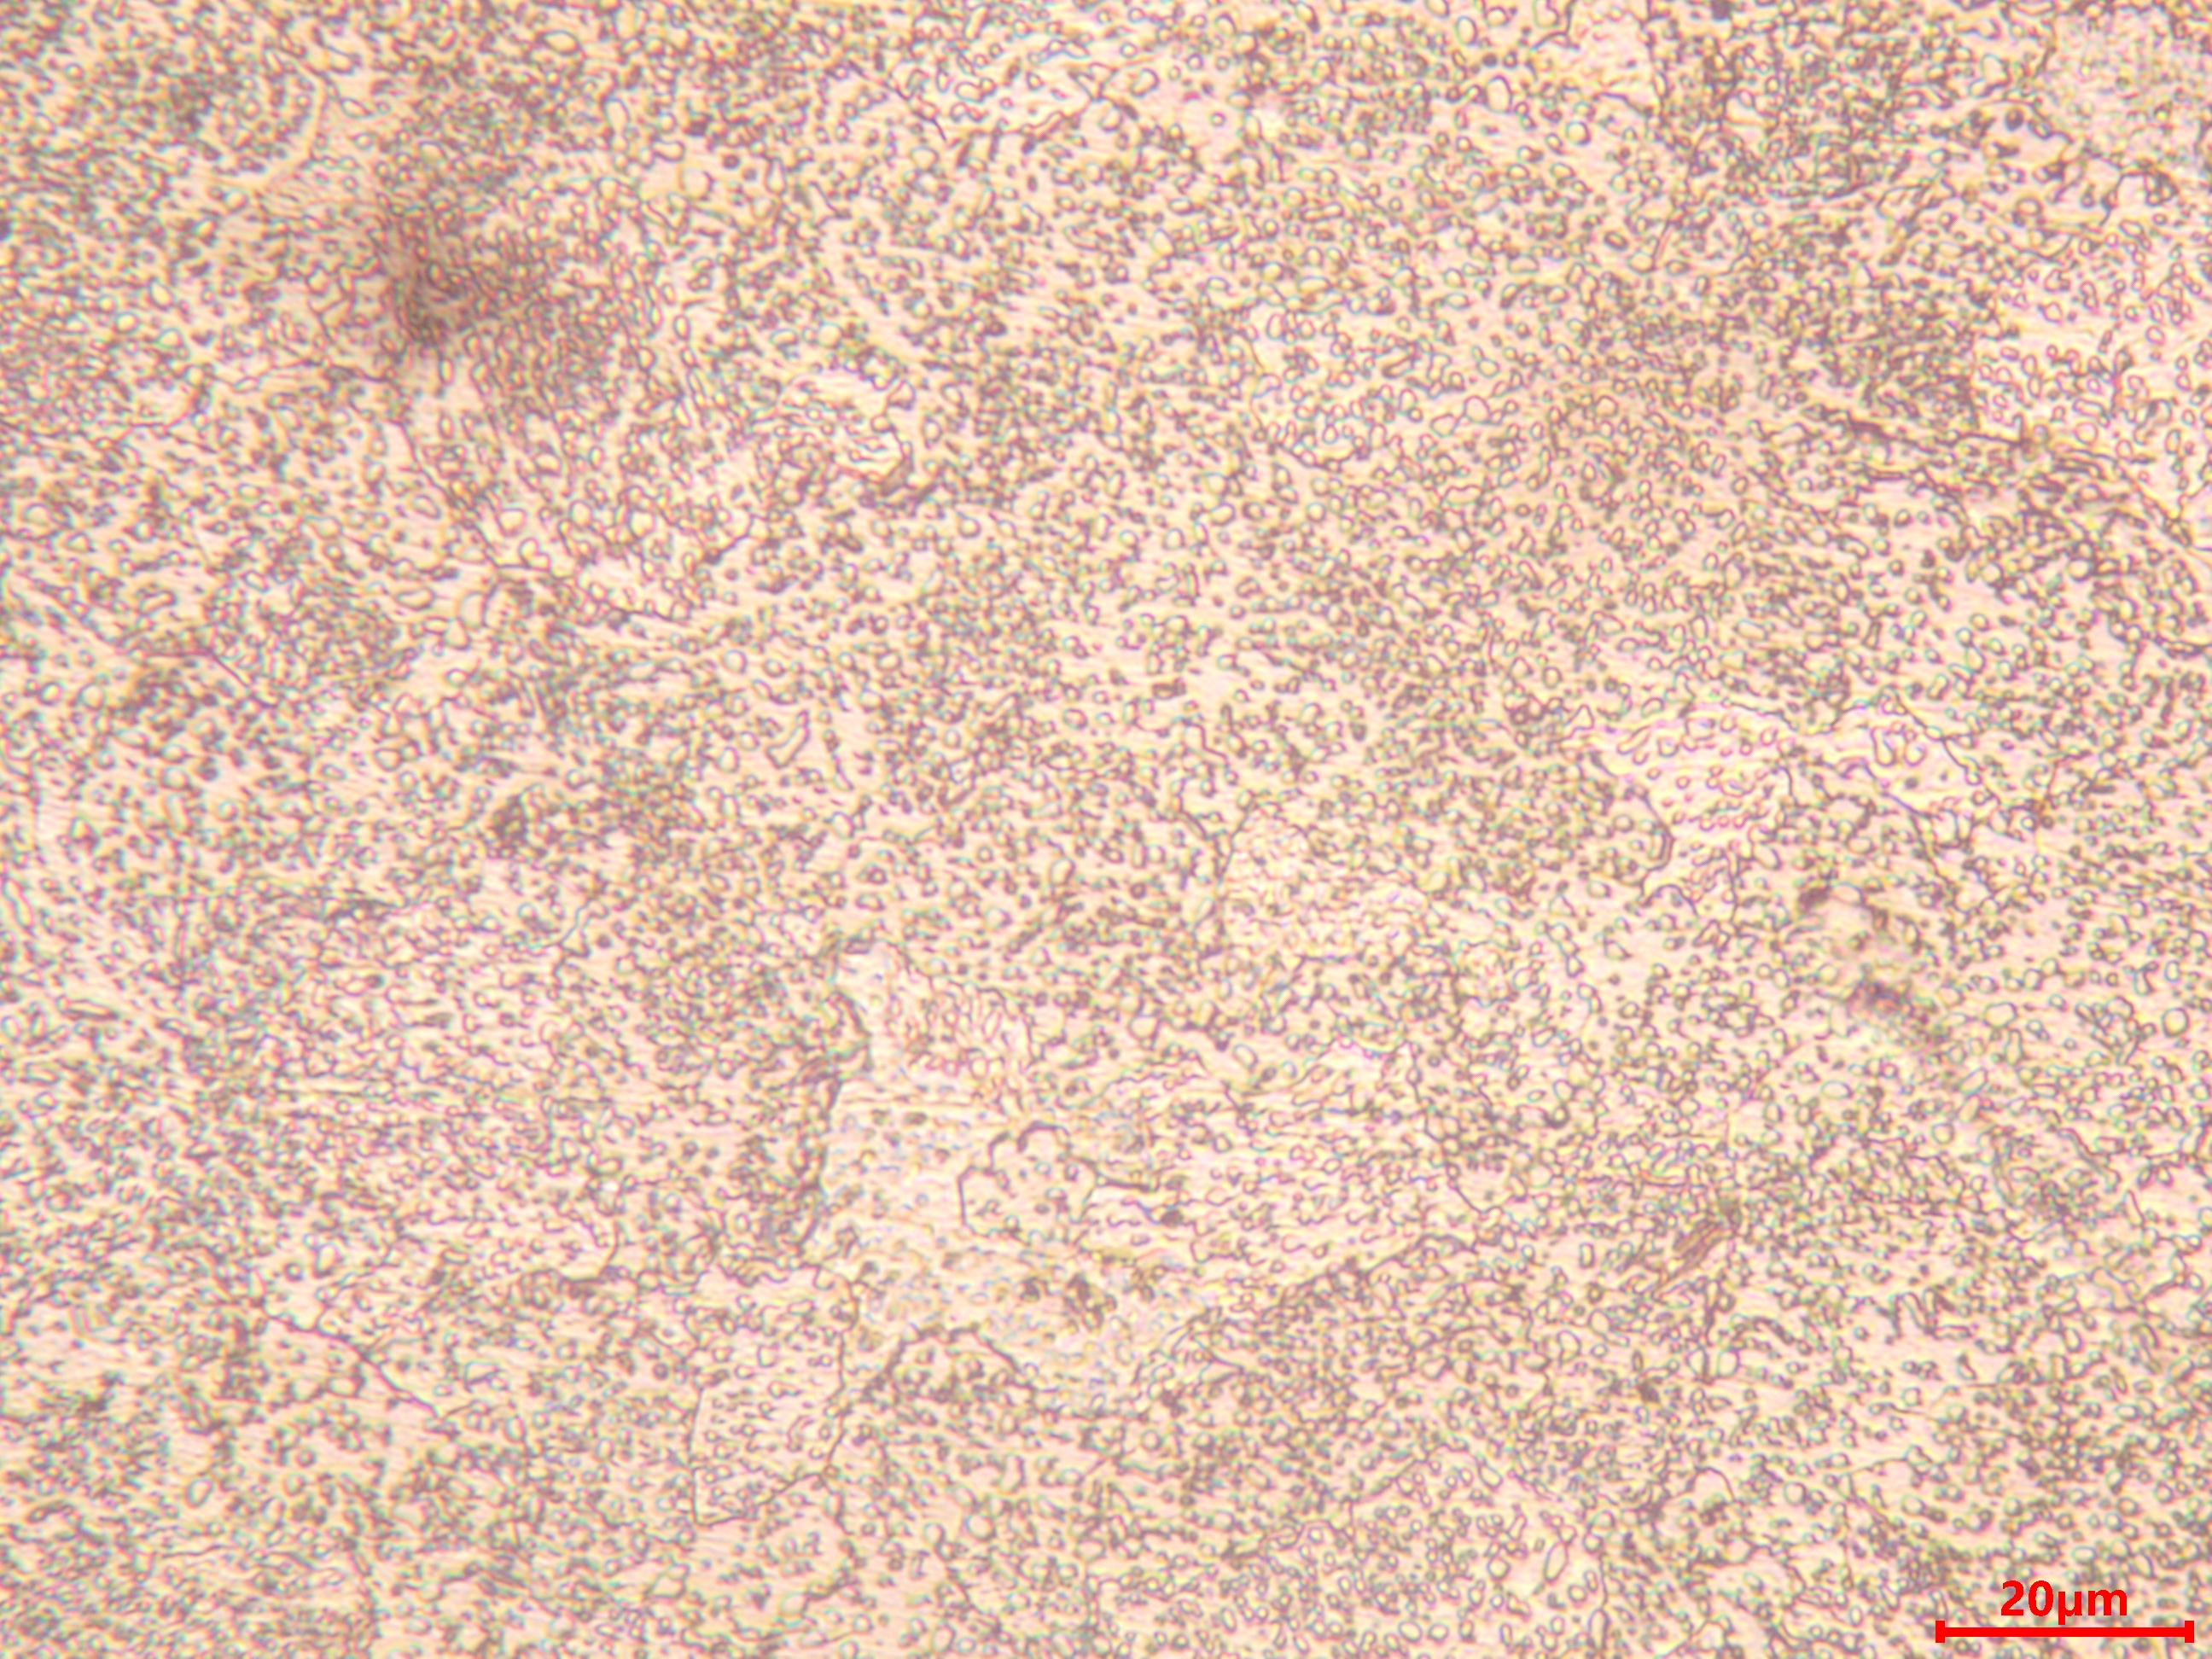
\includegraphics[height=24mm]{img/A1/25_500x.jpg}}
        \caption{T12 钢球化退火显微组织\label{fig:n12}}
    \end{figure}

    \subsubsection{T12 钢 \SI{780}{\degreeCelsius} 水淬 $+$ 低温回火\label{ss2:t12_780}}
    从\fgref{fig:n13} 可知,图中主要的组织为细小的针状马氏体加颗粒状亮白色渗碳体。
    \begin{figure}[!ht]
        \subfloat[$200\times{}$]{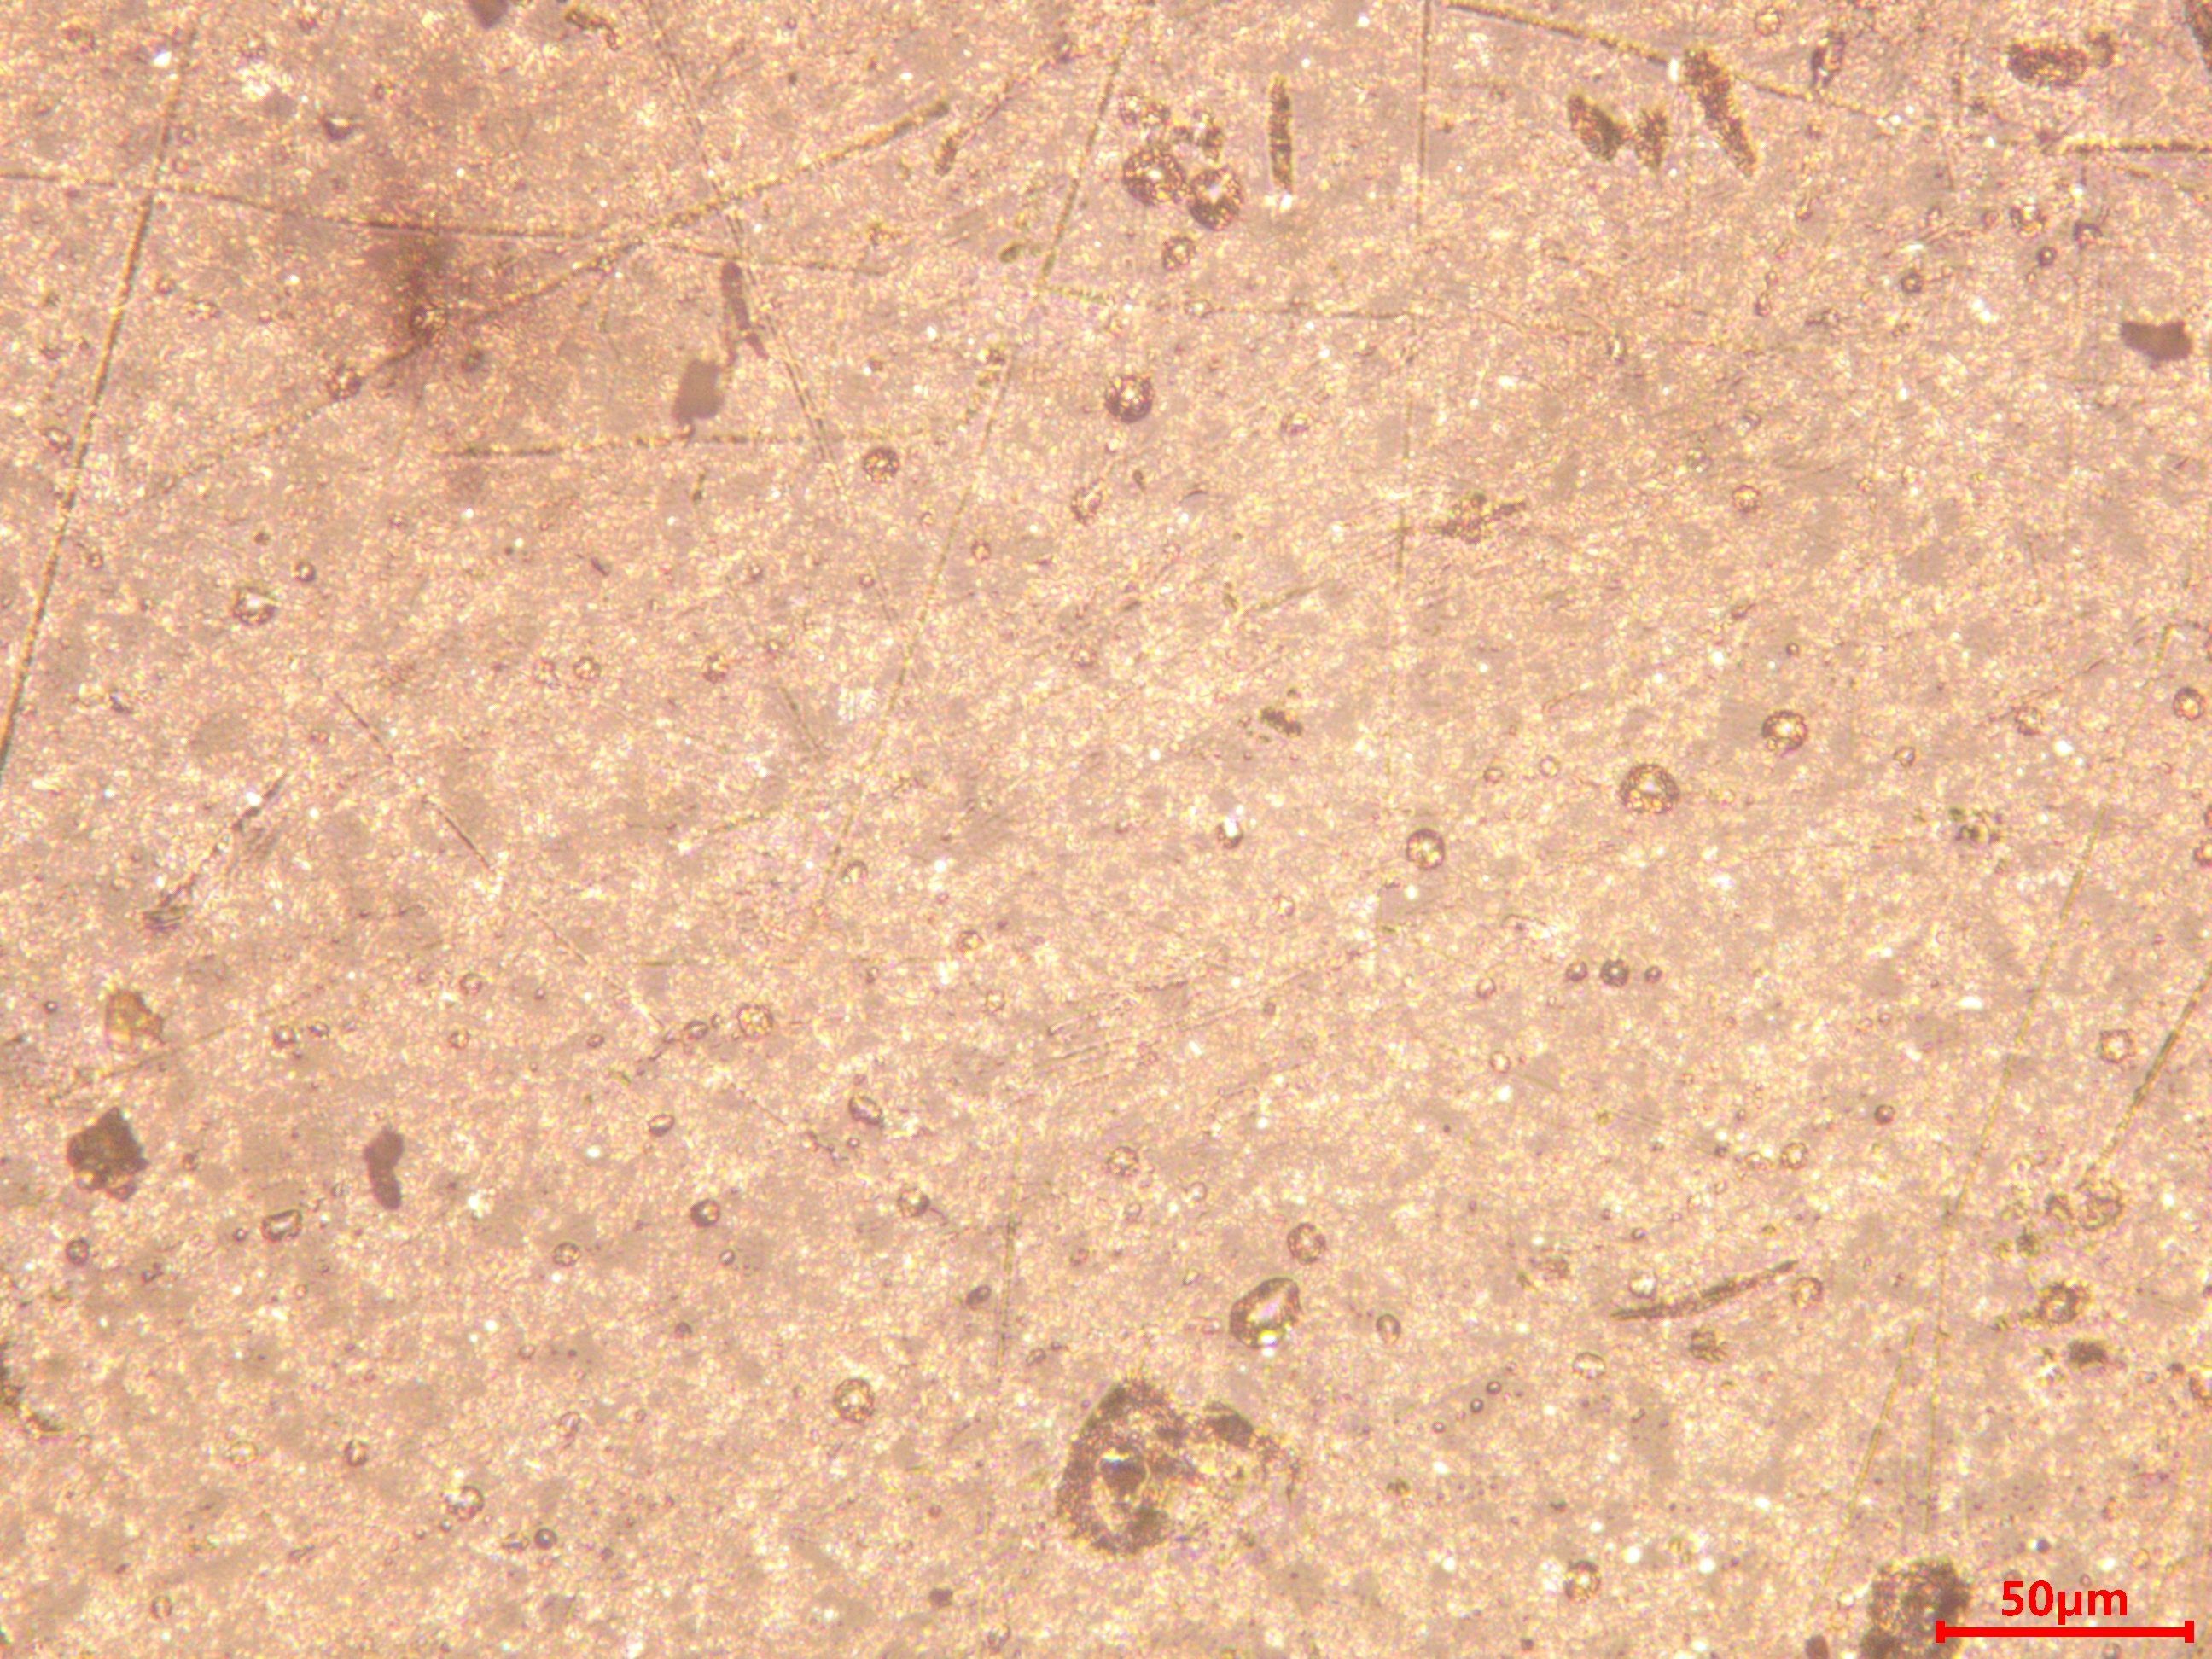
\includegraphics[height=24mm]{img/A1/26_200x.jpg}}\hspace{20pt}
        \subfloat[$500\times{}$]{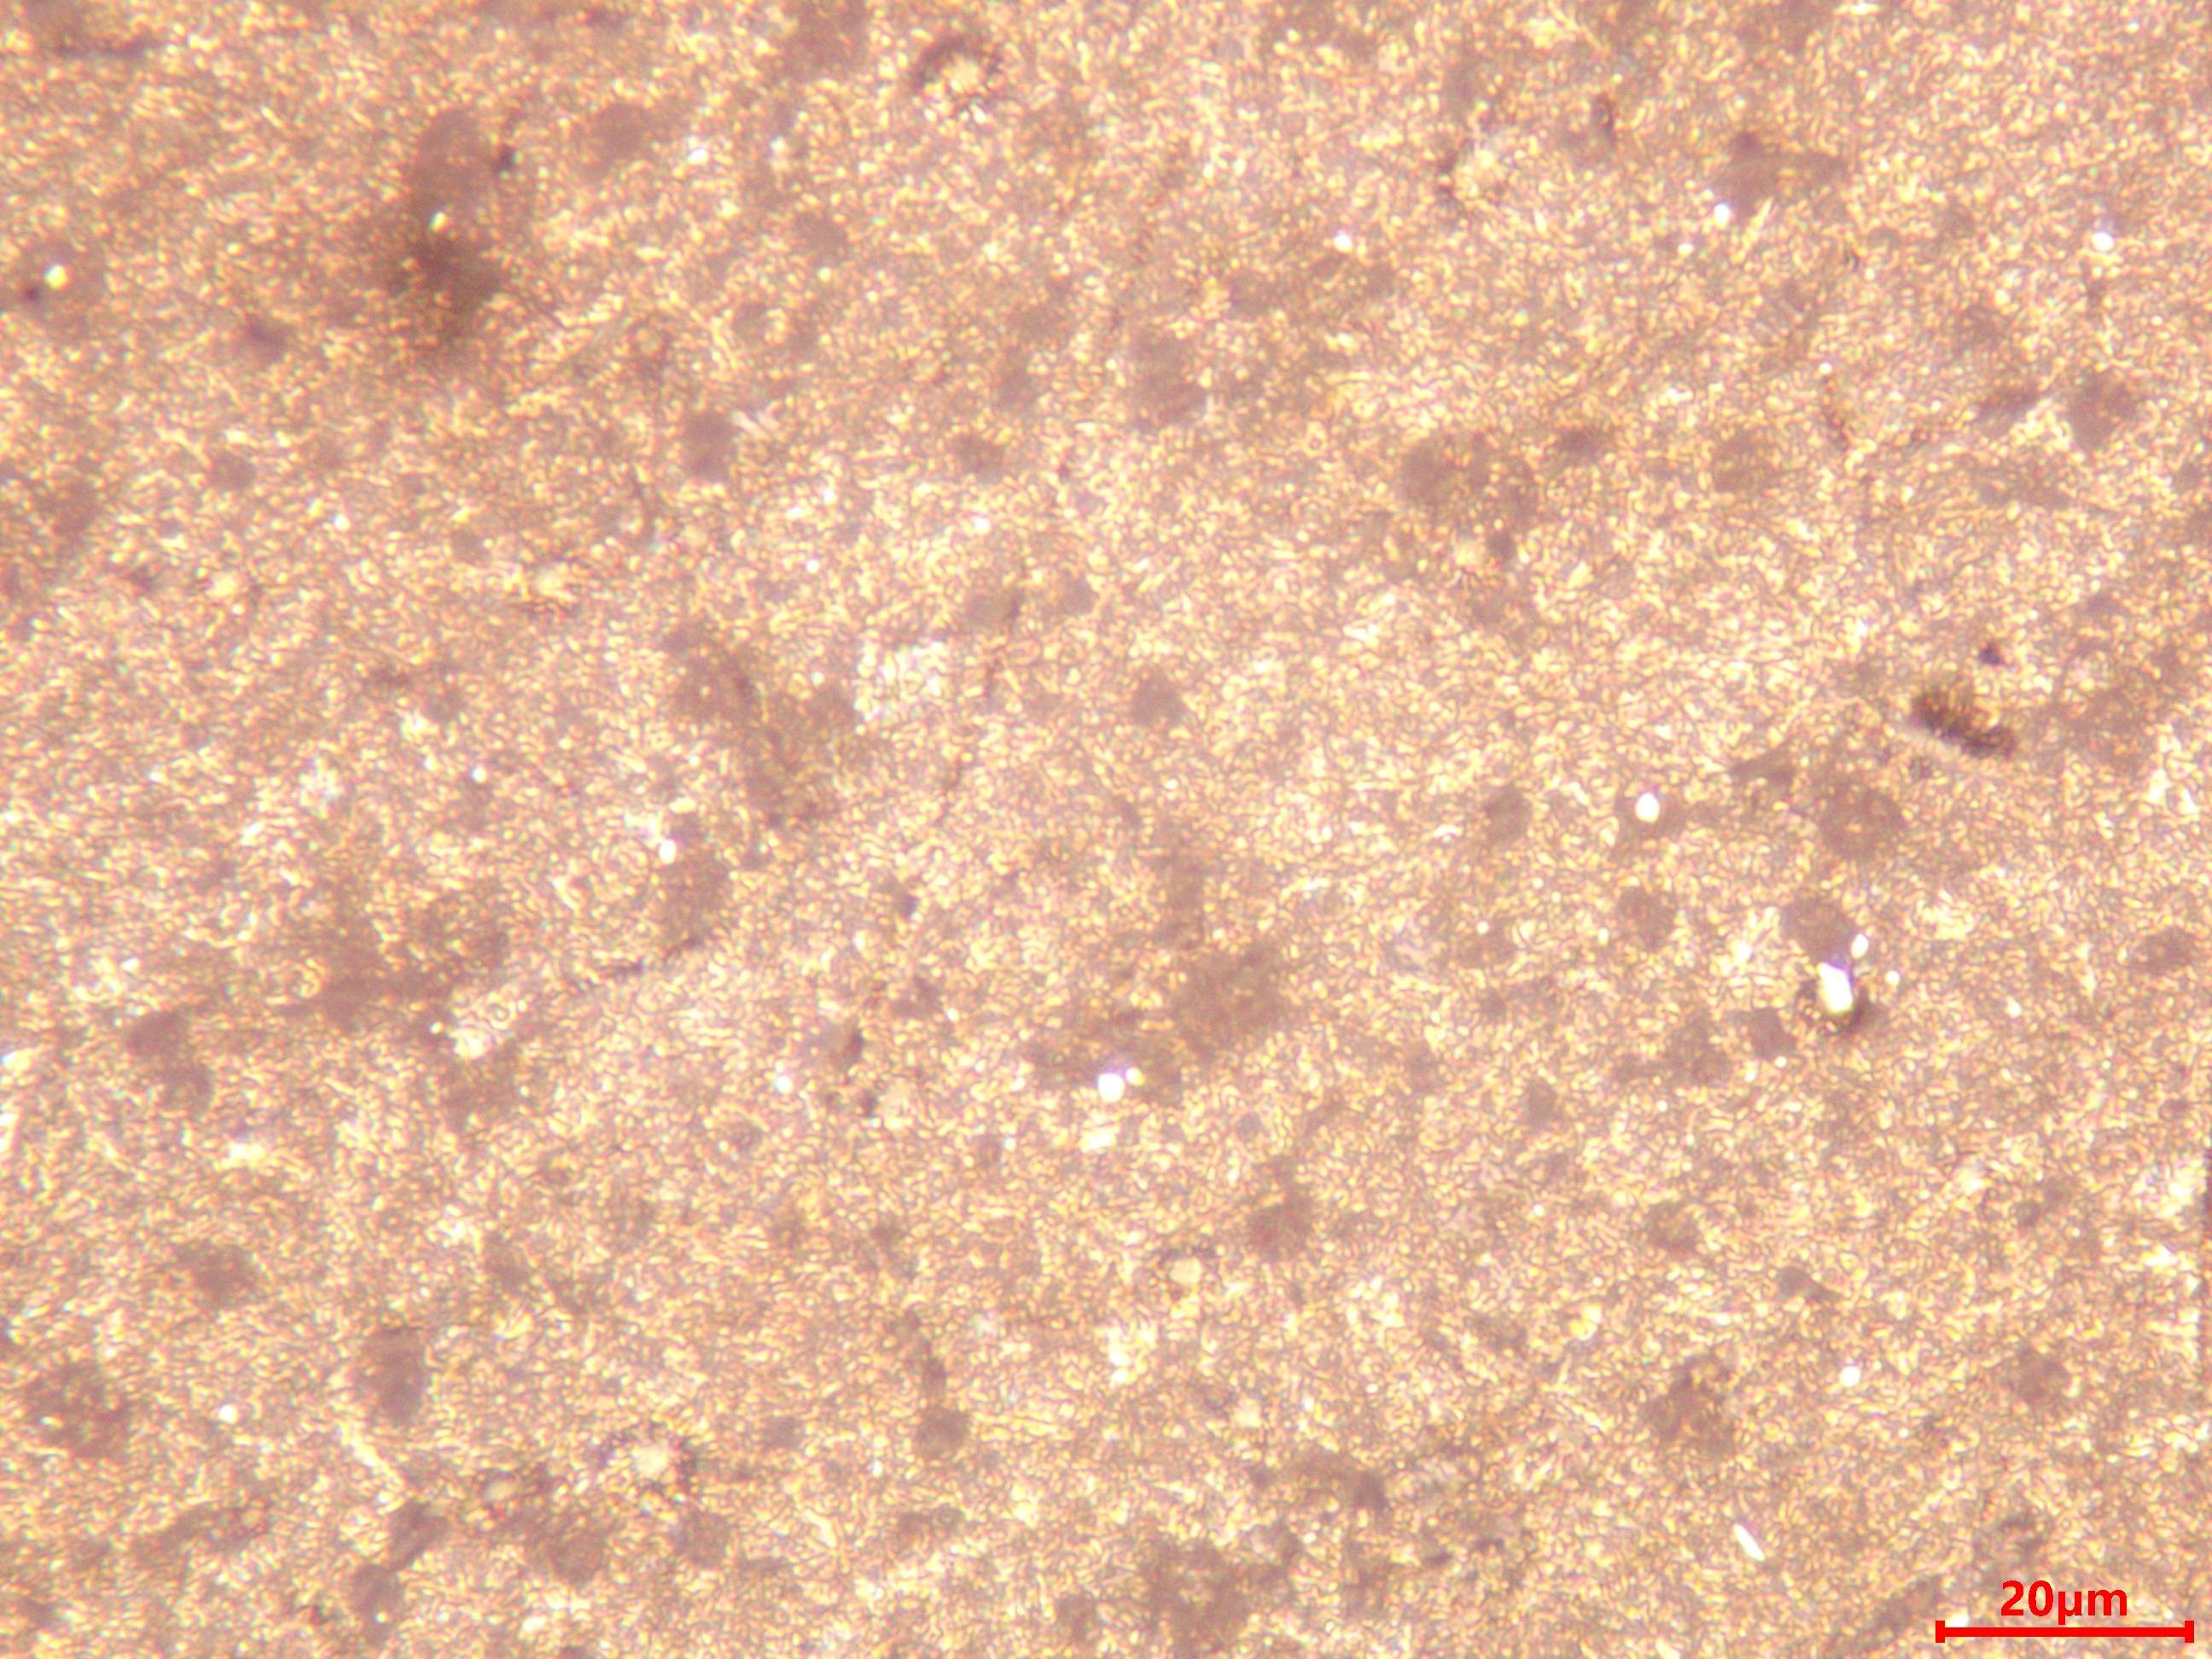
\includegraphics[height=24mm]{img/A1/26_500x.jpg}}
        \caption{T12 钢 \SI{780}{\degreeCelsius} 水淬 $+$ 低温回火显微组织\label{fig:n13}}
    \end{figure}

    \subsubsection{T12 钢 \SI{1100}{\degreeCelsius} 水淬 $+$ 低温回火\label{ss2:t12_1100}}
    从\fgref{fig:n14} 可知,图中主要的组织为粗片的马氏体与亮白色残余奥氏体。\par
    对比 \Nameref{ss2:t12_780} 和 \Nameref{ss2:t12_1100},可知,由于同为低温回火,所以最后的组织组成均为马氏体。但由于淬火的温度不同,组织的形态的并不相同。更高温度的淬火使马氏体的形态更加粗大。
    \begin{figure}[!ht]
        \subfloat[$200\times{}$]{\includegraphics[height=24mm]{img/A1/27_200x.jpg}}\hspace{20pt}
        \subfloat[$500\times{}$]{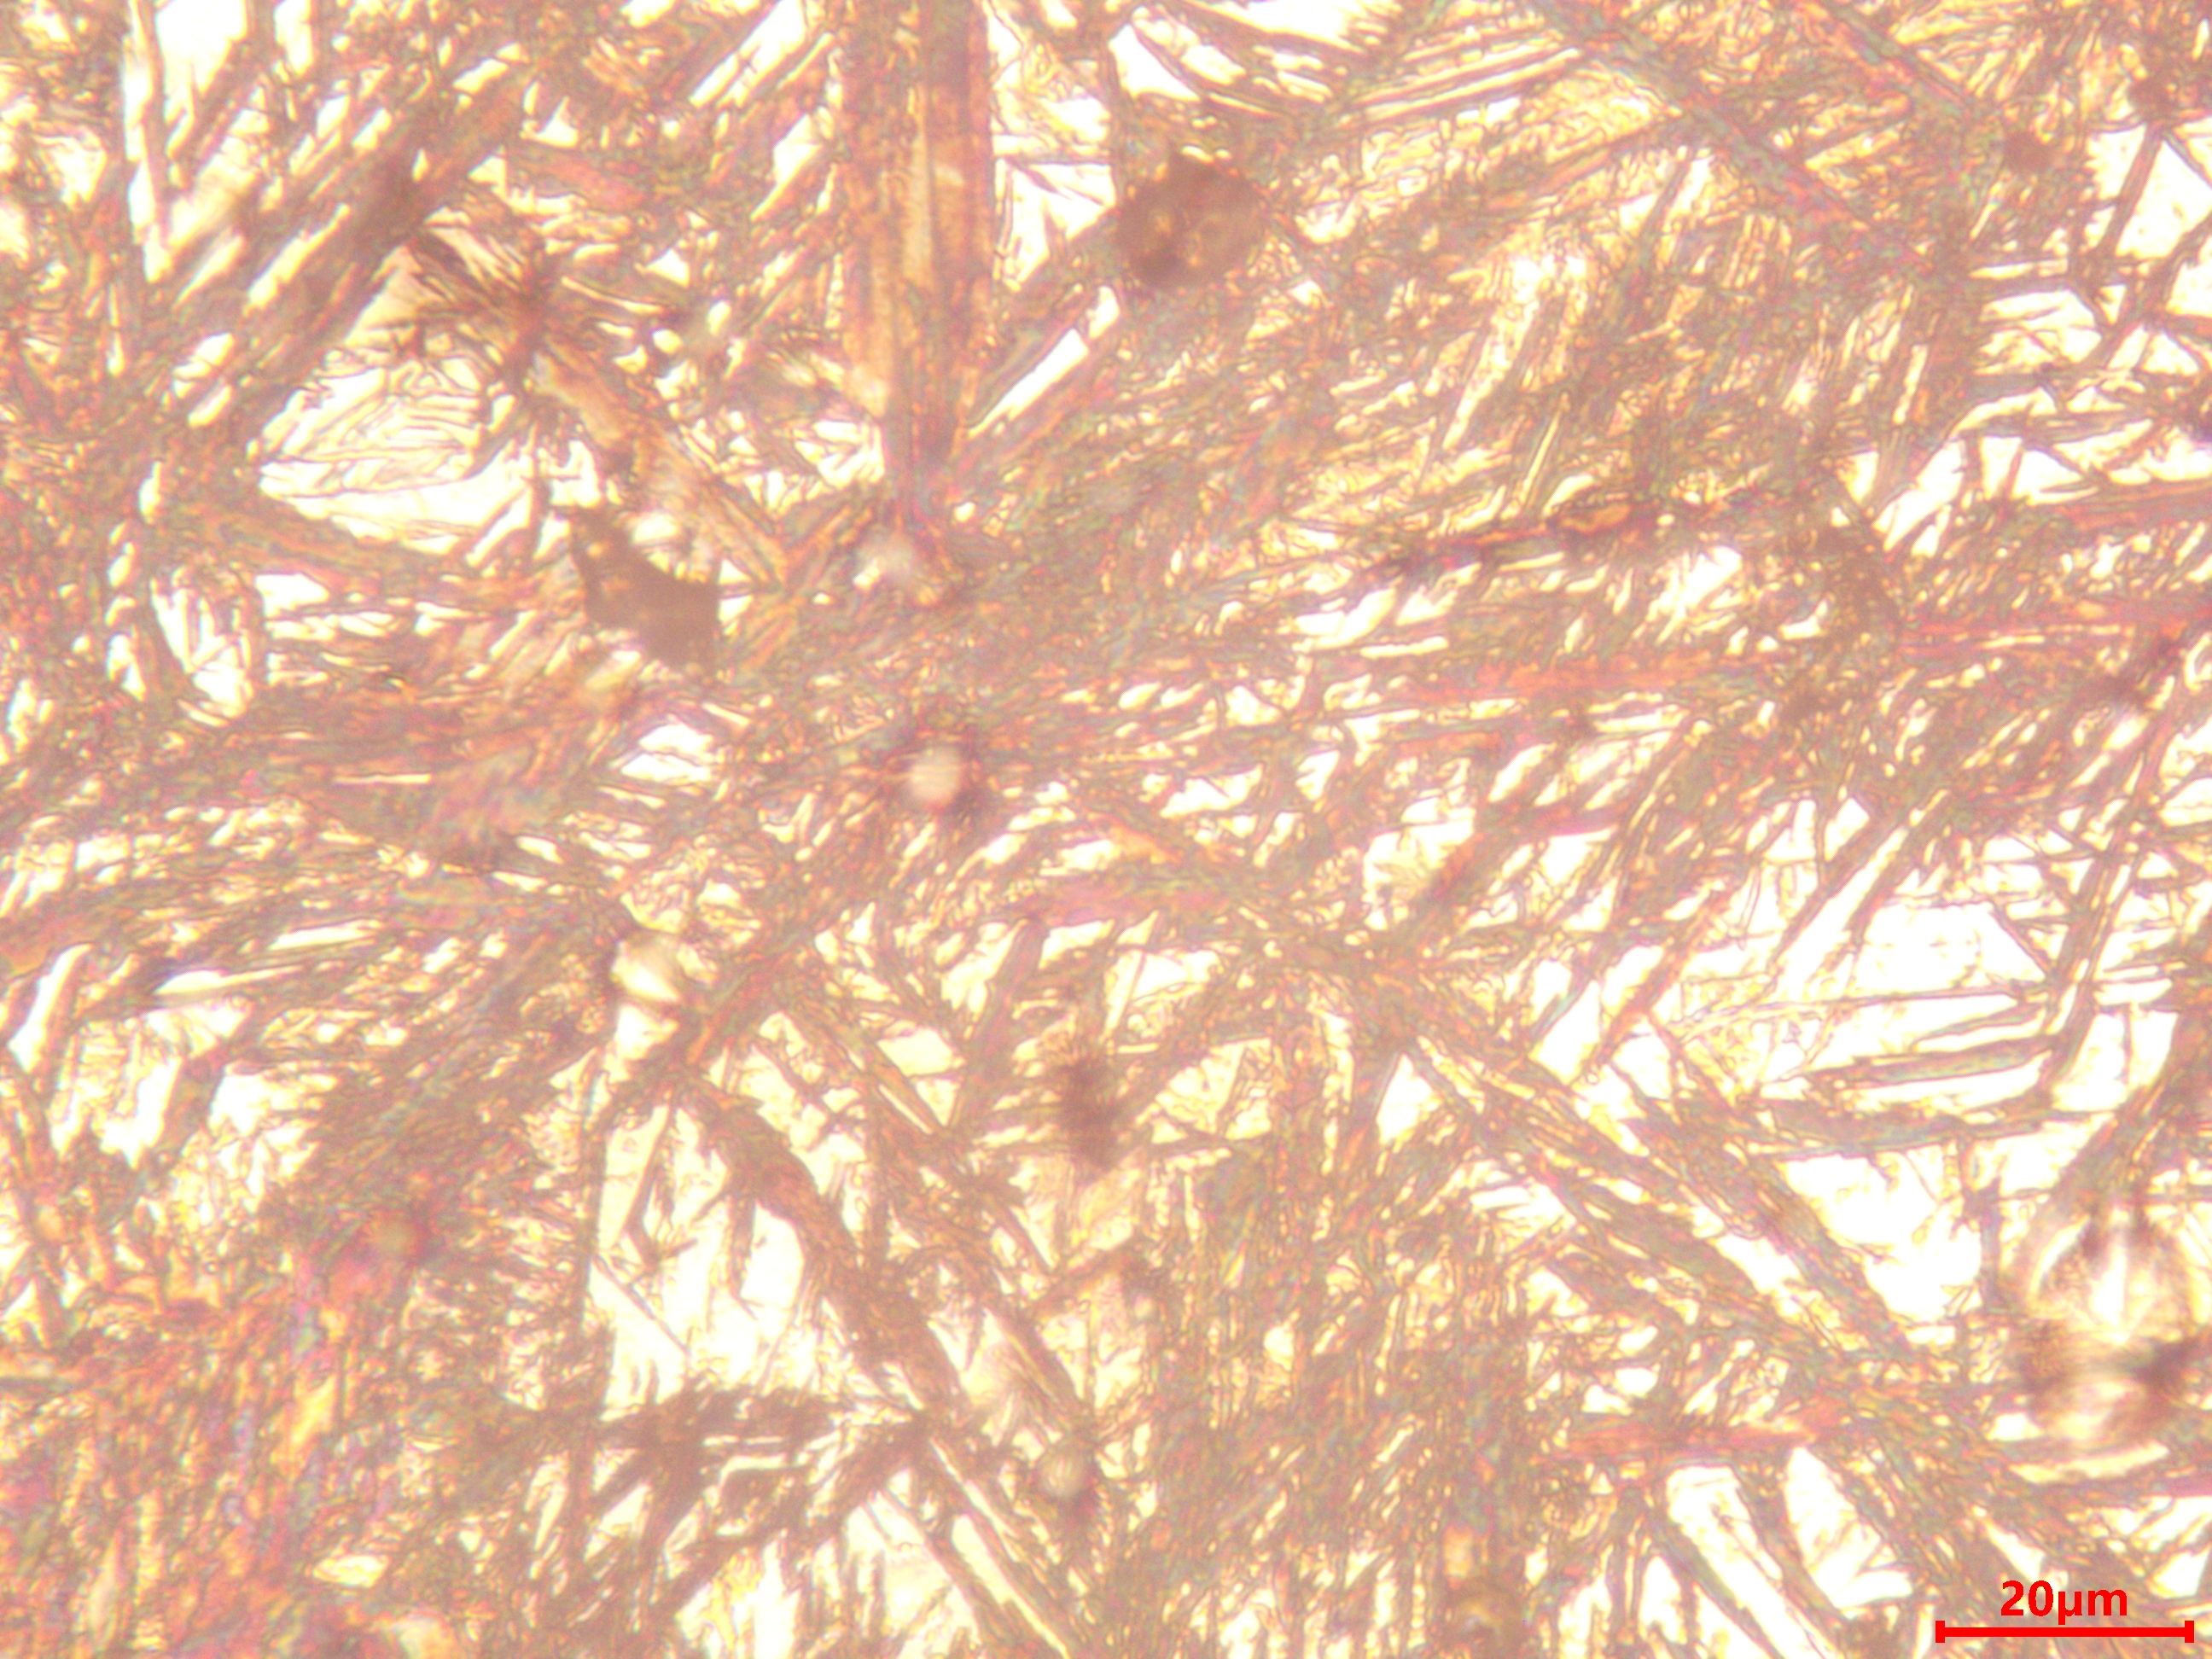
\includegraphics[height=24mm]{img/A1/27_500x.jpg}}
        \caption{T12 钢 \SI{1100}{\degreeCelsius} 水淬 $+$ 低温回火显微组织\label{fig:n14}}
    \end{figure}
\section{实验思考与讨论}
\begin{enumerate}
    \item \thinking{使用金相显微镜的一般步骤及注意事项是什么?}{\begin{enumerate}
        \item 将待观察的试样放置于载物台上,调节显微镜粗调手轮缓慢调节物镜与载物台的距离,使物镜与样品之间达到观察所需最小距离(调节过程必须缓慢,避免物镜直接撞击接触到试样)。此时观察目镜,目镜中出现影像,再调节微调手轮,直至影像清晰;
        \item 通过调节孔径光阑、视场光阑,得到最佳观察亮度。
        \item 通过调节载物台纵向和横向移动手柄以移动试样,改变观察区域,不得直接用手移动试样(对于倒置显微镜,如需观察工作台通光孔以外区域时可以提起试样,悬空转动试样,将该区域放置在通光孔中央,继续观察或者调整工作台位置后再进行观察)。
    \end{enumerate}}
    \item \thinking{在铁碳合金中观察到的渗碳体有几种形态?它们分别在什么情况下存在?}{在平衡组织中存在着三种形态的渗碳体:一次渗碳体、二次渗碳体和三次渗碳体。一次渗碳体主要在过共晶白口铸铁中出现,呈板条状。二次渗碳体则主要存在于过共析钢和亚共晶白口铁中。在过共析钢的显微组织中,二次渗碳体呈现白色网状结构,分布在晶界上;而在亚共晶白口铸铁中,由于二次渗碳体附着在珠光体表面,难以辨别。三次渗碳体主要出现在工业纯铁中,数量极少,通常无法观察到其形态。}
    \item \thinking{以 $\omega_C = 0.45\%$ 的铁碳合金为例,画出其缓慢冷却时的冷却曲线,并分析其组织变化过程。}{首先发生液体向高温铁素体的转变,$L \rightarrow \delta$ 继续降温,高温铁素体与液态金属发生包晶反应,$\delta + L \rightarrow \gamma$ 继续降温,残留液态金属向奥氏体转变,$L \rightarrow \gamma$ 继续降温至 Ac3 温度,奥氏体开始发生珠光体转变,$\gamma \rightarrow P + F$ 继续降温至 Ac1 温度,残留奥氏体完成珠光体转变,$\gamma \rightarrow P + F$ 至 Ac1 以下继续降温,不再有组织结构的改变,只是珠光体晶粒的生长。}
    \item \thinking{论述含碳量对铁碳合金的力学性能的影响。}{随着碳含量的增加,铁素体和珠光体中的碳含量增加,使得材料的硬度和强度增加。这是因为碳能够固溶在铁中形成固溶体,使得晶格变得更加紧密,增加了材料的硬度和强度。低碳钢通常具有较好的韧性,因为低碳含量有利于减少脆性相的形成,如渗碳体。随着碳含量的增加,脆性相的形成增加,导致材料的韧性降低。高碳钢具有较高的脆性,主要是由于高碳含量导致渗碳体的形成。渗碳体在晶界和晶粒内部形成裂纹,从而导致材料的脆性增加。}
\end{enumerate}